%%%%%%%%%%%%%%%%%%%%%%%%%%%%%%%%%%%%%%%%%%%%%%%%%%%%%%%%%%%%%%%%%%%%
%
%   Style for CMS Computing / Physics Technical Design Reports
%
%   Lucas Taylor  4 Feb 2005,   Revised  12 Oct 2005
%
%%%%%%%%%%%%%%%%%%%%%%%%%%%%%%%%%%%%%%%%%%%%%%%%%%%%%%%%%%%%%%%%%%%%

%  the following line is edited by the tdr script to change or to pass
%  additional options:
\documentclass[12pt,twoside,a4paper,an,final]{cms-tdr}
\def\svnVersion{}

%%%%%%%%%%%%%%%%%%%%%%%%%%%%%%%%%%%%%%%%%%%%%%%%%%%%%%%%%%%%%%%%%%%%

\begin{document}
%%%%%%%%%%%%%%%%%%%%%%%%%%%%%%%%%%%%%%%%%%%%%%%%%%%%%%%%%%%%%%%%%%%%
%
%  Common definitions
%
%  N.B. use of \providecommand rather than \newcommand means
%       that a definition is ignored if already specified
%
%                                              L. Taylor 18 Feb 2005
%%%%%%%%%%%%%%%%%%%%%%%%%%%%%%%%%%%%%%%%%%%%%%%%%%%%%%%%%%%%%%%%%%%%


%%%%%%%%%%%%%%%%%%%%%%%%%%%%%%%%%%%%%%%%%%%%%%%%%%%%%%%%%%%%%%%%%%%%
%
% Hyphenations (only need to add here if you get a nasty word break)
%
\hyphenation{had-ron-i-za-tion}
\hyphenation{cal-or-i-me-ter}
\hyphenation{de-vices}
%
% Hyphenations-end
% \RCS$Revision: 230053 $
\RCS$HeadURL: svn+ssh://svn.cern.ch/reps/tdr2/notes/AN-14-062/trunk/AN-14-062.tex $
\RCS$Id: AN-14-062.tex 230053 2014-03-05 06:58:25Z syu $
%%%%%%%%%%%%% local definitions %%%%%%%%%%%%%%%%%%%%%
% This allows for switching between one column and two column (cms@external) layouts
% The widths should  be modified for your particular figures. You'll need additional copies if you have more than one standard figure size.
\newlength\cmsFigWidth
\ifthenelse{\boolean{cms@external}}{\setlength\cmsFigWidth{0.85\columnwidth}}{\setlength\cmsFigWidth{0.4\textwidth}}
\ifthenelse{\boolean{cms@external}}{\providecommand{\cmsLeft}{top}}{\providecommand{\cmsLeft}{left}}
\ifthenelse{\boolean{cms@external}}{\providecommand{\cmsRight}{bottom}}{\providecommand{\cmsRight}{right}}
\ifthenelse{\boolean{cms@external}}{\providecommand{\cmsLeftU}{Top\xspace}}{\providecommand{\cmsLeftU}{Top left\xspace}}
\ifthenelse{\boolean{cms@external}}{\providecommand{\cmsRightU}{middle\xspace}}{\providecommand{\cmsRightU}{Top right\xspace}}



%%%%%%%%%%%%%%%  Title page %%%%%%%%%%%%%%%%%%%%%%%%
\cmsNoteHeader{Final Report: MOST 107-2813-C-008-053-M} % This is over-written in the CMS environment: useful as preprint no. for export versions
\newcommand{\mJ}{\ensuremath{m_{\text{jet}}}\xspace}
\newcommand{\qqbarpr}{\ensuremath{\Pq\Paq^{(\prime)}}\xspace}
\newcommand{\nsubj}{\ensuremath{\tau_{21}}}
\newcommand{\Gbulk}{\ensuremath{\mathrm{G}_\text{bulk}}\xspace}
\newcommand{\Vprime}{\ensuremath{\mathrm{V}'}\xspace}
\providecommand{\NA}{\ensuremath{\text{---}}\xspace}
\makeatletter
\newcommand*{\rom}[1]{\expandafter\@slowromancap\romannumeral #1@}

\newcommand{\PV}{\ensuremath{\mathrm{V}}}
\providecommand{\NA}{---}
\newcommand{\LOWSBLOW}{40\xspace}
\newcommand{\SRLOW}{65\xspace}
\newcommand{\SRMIDDLE}{85\xspace}
\newcommand{\SRHIGH}{105\xspace}
\newcommand{\HIGHSBLOW}{135\xspace}
\newcommand{\HIGHSBHIGH}{150\xspace}
\newcommand{\SFWTAGHPWPT} {\ensuremath{0.95\pm0.06}\xspace}
\newcommand{\SFWTAGLPWPT} {\ensuremath{1.25\pm0.32}\xspace}
\newcommand{\SFWTAGHPWPL} {\ensuremath{1.01\pm0.03}\xspace}
\newcommand{\WMASSDATAWPT} {\ensuremath{84.6\pm0.7}\xspace}
\newcommand{\WRESDATAWPT} {\ensuremath{8.2\pm0.7}\xspace}
\newcommand{\WMASSMCWPT} {\ensuremath{85.1\pm0.2}\xspace}
\newcommand{\WRESMCWPT} {\ensuremath{7.8\pm0.3}\xspace}
\newcommand{\LUMIUNCERT} {2.7\%\xspace}
\newcommand{\Wo}{\PW\xspace}%                                                                                                                 
\newcommand{\Zo}{\cPZ\xspace}%                                                                                                                
\newcommand{\Vo}{\ensuremath{\mathrm{V}}\xspace}%                                                                                             
\newcommand{\mX}{\ensuremath{\text{M}_{\text{X}}}}%                                                                                           
\newcommand{\wX}{\ensuremath{\Gamma_{\text{X}}}}%                                                                                             
\newcommand{\mVV}{\ensuremath{m_{\Vo\Vo}}\xspace}%                                                                                            
\newcommand{\mjj}{\ensuremath{m_\mathrm{jj}}}%                                                                                                
\newcommand{\mJ}{\ensuremath{m_{\text{jet}}}}%                                                                                                
\newcommand{\nsubj}{\ensuremath{\tau_{21}}}%                                                                                                  
\newcommand{\ktilde}{\ensuremath{k/\overline{M}_\mathrm{Pl}}\xspace}%                                                                         
\newcommand{\amcatnlo}{{\MADGRAPH{}5\_a\MCATNLO}\xspace}
\newcommand{\BulkG}{\ensuremath{\PXXG_{\text{bulk}}}\xspace}
\newcommand{\lnujet}{\ensuremath{\ell \nu}+jet\xspace}

\newcommand{\Wpr}{\ensuremath{\rm W^\prime}\xspace}
\newcommand{\Zpr}{\ensuremath{\rm Z^\prime}\xspace}
\renewcommand{\PTm}{\ensuremath{p_{\mathrm{T}}^{\text{miss}}}\xspace}
\newcommand\T{\rule[-.50em]{0pt}{1.50em}}


\newcommand{\Xtohh}{\ensuremath{\X\to\Ph\Ph}\xspace}

\newcommand{\qqbarpr}{\ensuremath{\Pq\Paq^({}'^){}}\xspace}
\newcommand{\lnujet}{\ensuremath{\ell \nu}+jet\xspace}
\newcommand{\lljet}{\ensuremath{\ell \ell}+jet\xspace}
\newcommand{\PV}{\ensuremath{\mathrm{V}}}
\newcommand{\nsubj}{\ensuremath{\tau_{21}}}%
\newcommand{\Vo}{\ensuremath{\mathrm{V}}\xspace}%
\newcommand{\mVV}{\ensuremath{m_{\Vo\Vo}}\xspace}%
\newcommand{\Grav}{\ensuremath{\PXXG_{\mathrm{bulk}}}}%
\newcommand{\ktilde}{\ensuremath{k/\overline{M}_\mathrm{Pl}}\xspace}%
\newcommand{\pb}{\ensuremath{\cmsSymbolFace{pb}}\xspace}
\newcommand{\X}{\ensuremath{\cmsSymbolFace{X}}\xspace}
\newcommand{\A}{\ensuremath{\cmsSymbolFace{A}}\xspace}
\newcommand{\V}{\ensuremath{\cmsSymbolFace{V}}\xspace}
\newcommand{\h}{\ensuremath{\cmsSymbolFace{h}}\xspace}
\renewcommand{\PW}{\ensuremath{\cmsSymbolFace{W}}\xspace}
\newcommand{\XtoVh}{\ensuremath{\X\to\V\Ph}\xspace}
\newcommand{\XtoZh}{\ensuremath{\X\to\Z\Ph}\xspace}
\newcommand{\XtoWh}{\ensuremath{\X\to\PW\Ph}\xspace}
\newcommand{\AtoZh}{\ensuremath{\A\to\Z\Ph}\xspace}
\newcommand{\htobb}{\ensuremath{\Ph\to\bbbar}\xspace}
\newcommand{\Ztoll}{\ensuremath{\Z\to\ell\ell}\xspace}
\newcommand{\Ztoee}{\ensuremath{\Z\to\Pe\Pe}\xspace}
\newcommand{\Ztomm}{\ensuremath{\Z\to\mu\mu}\xspace}
\newcommand{\Ztonn}{\ensuremath{\Z\to\nu\nu}\xspace}
\newcommand{\Atollbb}{\ensuremath{\A\to\Z\Ph\to{\ell\ell}\bbbar}\xspace}
\newcommand{\Xtollbb}{\ensuremath{\X\to\Z\Ph\to{\ell\ell}\bbbar}\xspace}
\newcommand{\Xtoeebb}{\ensuremath{\X\to\Z\Ph\to{\Pe\Pe}\bbbar}\xspace}
\newcommand{\Xtommbb}{\ensuremath{\X\to\Z\Ph\to{\mu\mu}\bbbar}\xspace}
\newcommand{\Xtolnbb}{\ensuremath{\X\to\PW\Ph\to{\ell\nu}\bbbar}\xspace}
\newcommand{\Xtoenbb}{\ensuremath{\X\to\PW\Ph\to{\Pe\nu}\bbbar}\xspace}
\newcommand{\Xtomnbb}{\ensuremath{\X\to\PW\Ph\to{\mu\nu}\bbbar}\xspace}
\newcommand{\Xtonnbb}{\ensuremath{\X\to\Z\Ph\to{\nu\nu}\bbbar}\xspace}
\renewcommand{\PHpm}{\ensuremath{\PH^\pm}\xspace}
\newcommand{\Zh}{\ensuremath{\Z\Ph}\xspace}
\newcommand{\Wh}{\ensuremath{\PW\Ph}\xspace}
\newcommand{\VH}{\ensuremath{\V\Ph}\xspace}
\newcommand{\VV}{\ensuremath{\V\V}\xspace}
\newcommand{\ST}{\ensuremath{\text{ST}}\xspace}
\newcommand{\Vjets}{\ensuremath{\V\text{+jets}}\xspace}
\newcommand{\mVH}{\ensuremath{m_{\VH}}\xspace}
\newcommand{\mX}{\ensuremath{m_{\X}}\xspace}
\newcommand{\mT}{\ensuremath{m_{\text{T}}}\xspace}
\newcommand{\mA}{\ensuremath{m_{\A}}\xspace}
\newcommand{\mh}{\ensuremath{m_{\Ph}}\xspace}
\newcommand{\mHpm}{\ensuremath{m_{\PHpm}}\xspace}
\newcommand{\mt}{\ensuremath{m_{\PQt}}\xspace}
\newcommand{\mtX}{\ensuremath{m_{\PQt}^{\X}}\xspace}
\newcommand{\ttbarV}{\ensuremath{\ttbar V\xspace}}
\newcommand{\mbb}{\ensuremath{m_{\PQb\PQb}}\xspace}
\newcommand{\mll}{\ensuremath{m_{\ell\ell}}\xspace}
\newcommand{\mllbb}{\ensuremath{m_{\ell\ell\PQb\PQb}}\xspace}
\newcommand{\mlnbb}{\ensuremath{m_{\ell\nu\PQb\PQb}}\xspace}
\newcommand{\mTnnbb}{\ensuremath{m^T_{\nu\nu\PQb\PQb}}\xspace}
\newcommand{\cosba}{\ensuremath{\cos(\beta-\alpha)}\xspace}
\newcommand{\B}{\ensuremath{\mathcal{B}}}
\newcommand{\fb}{\ensuremath{\,\text{fb}}\xspace}
\newcommand{\Zb}{\ensuremath{\Z+\PQb}\xspace}
\newcommand{\Zbbbar}{\ensuremath{\Z+\bbbar}\xspace}
\newcommand{\qqbar}{\ensuremath{\cPq\cPaq}\xspace}
\newcommand{\MHT}{\ensuremath{H_\text{T}^\text{miss}}\xspace}

\renewcommand{\HGG}{\ensuremath{\Ph\rightarrow\gamma\gamma}\xspace}
\newcommand{\Hbb}{\ensuremath{\Ph\rightarrow\PQb\PAQb}\xspace}
\newcommand{\mzp}{\ensuremath{m_{\PZpr}}\xspace}
\renewcommand{\Az}{\ensuremath{\cmsSymbolFace{A}}\xspace}
\newcommand{\ptm}{\ensuremath{p_{\mathrm{T}}^{\text{miss}}}\xspace}
\renewcommand{\MET}{\ptm}
\renewcommand{\ETm}{\ptm}
\newcommand{\maz}{\ensuremath{m_{\Az}}\xspace}
\newcommand{\mdm}{\ensuremath{m_{\chi}}\xspace}
\newcommand{\gzp}{\ensuremath{g_{\PZpr}}\xspace}
\newcommand{\MADGRAPHAMC} {\MADGRAPH{}5\_a\MCATNLO}
\newcommand{\x}{\ensuremath{\phantom{0}}}

\providecommand{\Ph}{\ensuremath{\cmsSymbolFace{h}}\xspace}
\providecommand{\PQb}{\cPqb}
\providecommand{\PQt}{\cPqt}
\providecommand{\PZ}{\ensuremath{\cmsSymbolFace{Z}}\xspace}
\providecommand{\PW}{\ensuremath{\cmsSymbolFace{W}}\xspace}
\newcommand{\ttjets}{\ensuremath{\cPqt\overline{\cPqt}}+jets\xspace}
\newcommand{\wjets}{\PW+jets\xspace}
\newcommand{\bjet}{\cPqb~jet\xspace}
\newcommand{\bjets}{\cPqb~jets\xspace}
\newcommand{\sm}{the standard model\xspace}
\newcommand{\mc}{Monte Carlo\xspace}
\newcommand{\com}{13\TeV\xspace}
\newcommand{\intLumi}{35.9\fbinv}

\newcommand{\Hbbt}{double-\cPqb\,tagger\xspace}
\newcommand{\Sjbt}{subjet \PQb\,tagger\xspace}
\newcommand{\GRS}{\ensuremath{\mathrm{G}_\mathrm{RS}}\xspace}
\newcommand{\mjj}{\ensuremath{m_{\text{jj}}}\xspace}
\newcommand{\mjjs}{\ensuremath{m_{\text{jj}}^{\text{red}}}\xspace}
\newcommand{\Mjjs}{\ensuremath{m_{\text{jj}}^{\text{red}}}\xspace}
\newcommand{\mjjred}{\ensuremath{m_{\text{jj}}^{\text{red}}}\xspace}
\newcommand{\Mjjred}{\ensuremath{m_{\text{jj}}^{\text{red}}}\xspace}
\newcommand{\mH}{\ensuremath{m_{\text{\PH}}}\xspace}
\newcommand{\mx}{\ensuremath{m_{\text{X}}}\xspace}
\newcommand{\mux}{\ensuremath{\mu_{\text{X}}^{\text{CB}}}\xspace}
\newcommand{\nsub}{\ensuremath{\tau_{21}}\xspace}
\newcommand{\etaj}{\ensuremath{|\eta|}\xspace}
\newcommand{\deta}{\ensuremath{|\Delta\eta_{\text{jj}}|}\xspace}
\newcommand{\mjp}{\ensuremath{m_{\text{jet}}^{\text{pruned}}}\xspace}
\newcommand{\mjsd}{\ensuremath{m_{\text{jet}}^{\text{softdrop,puppi}}}\xspace}
\newcommand{\mj}{\ensuremath{m_{\text{jet}}}\xspace}
\newcommand{\mjone}{\ensuremath{m_{\text{j}_{1}}}\xspace}
\newcommand{\mjtwo}{\ensuremath{m_{\text{j}_{2}}}\xspace}
\newcommand{\LambdaR}{\ensuremath{\Lambda_{\text{R}}}\xspace}
\newcommand{\DeltaEta}{\ensuremath{\Delta\eta(\text{j}_{1}, \text{j}_{2})}\xspace}
\newcommand{\HH}{\PH\PH}
\newcommand{\sgx}{\ensuremath{\sigma_{\text{X}}^{\text{gaus}}}\xspace}
\newcommand{\scbx}{\ensuremath{\sigma_{\text{X}}^{\text{CB}}}\xspace}
\newcommand{\HbbHbb}{\ensuremath{\mathrm{\Hbb\Hbb}}\xspace} 
\newcommand{\XHbbHbb}{\ensuremath{\mathrm{X}\rightarrow\PH\PH\rightarrow\bbbar\bbbar}\xspace}

\newcommand{\X}{\ensuremath{\cmsSymbolFace{X}}\xspace}
\newcommand{\V}{\ensuremath{\cmsSymbolFace{V}}\xspace}
\newcommand{\h}{\ensuremath{\cmsSymbolFace{H}}\xspace}
\renewcommand{\PW}{\ensuremath{\cmsSymbolFace{W}}\xspace}
\newcommand{\htobb}{\ensuremath{\PH\to\bbbar}\xspace}
\newcommand{\VH}{\ensuremath{\V\PH}\xspace}
\newcommand{\VV}{\ensuremath{\V\V}\xspace}
\newcommand{\ST}{\ensuremath{\text{t+X}}\xspace}
\newcommand{\Vjets}{\ensuremath{\V\text{+jets}}\xspace}
\newcommand{\mVH}{\ensuremath{m_{\VH}}\xspace}
\newcommand{\mtVH}{\ensuremath{m_{\VH}^\mathrm{T}}\xspace}
\newcommand{\mX}{\ensuremath{m_{\X}}\xspace}
\newcommand{\mH}{\ensuremath{m_{\PH}}\xspace}
\newcommand{\mj}{\ensuremath{m_{\mathrm{j}}}\xspace}
\newcommand{\B}{\ensuremath{\mathcal{B}}}
\newcommand{\gV}{\ensuremath{g_\text{V}}\xspace}
\newcommand{\cH}{\ensuremath{c_\text{H}}\xspace}
\newcommand{\cF}{\ensuremath{c_\text{F}}\xspace}
\newcommand{\MHT}{\ensuremath{H_\text{T}^\text{miss}}\xspace}
\newcommand{\MG}{\MADGRAPH{5}\_a\MCATNLO\xspace}

\newcommand{\Hbb}{\ensuremath{\PH\to\bbbar}\xspace}
\newcommand{\ttjets}{\ttbar+jets\xspace}
\newcommand{\intLumi}{35.9\fbinv}
\newcommand{\Hbbt}{double-\PQb\,tagger\xspace}
\newcommand{\mjj}{\ensuremath{m_{\text{jj}}}\xspace}
\newcommand{\mjjs}{\ensuremath{m_{\text{jj,red}}}\xspace}
\newcommand{\mjjred}{\ensuremath{m_{\text{jj,red}}}\xspace}
\newcommand{\mH}{\ensuremath{m_{\PH}}\xspace}
\newcommand{\nsub}{\ensuremath{\tau_{21}}\xspace}
\newcommand{\mjone}{\ensuremath{m_{\text{j}_{1}}}\xspace}
\newcommand{\mjtwo}{\ensuremath{m_{\text{j}_{2}}}\xspace}
\newcommand{\LambdaR}{\ensuremath{\Lambda_{\text{R}}}\xspace}
\newcommand{\DeltaEta}{\ensuremath{\Delta\eta(\text{j}_{1}, \text{j}_{2})}\xspace}
\newcommand{\PX}{\ensuremath{\cmsSymbolFace{X}}}
\newcommand{\mx}{\ensuremath{m_{\PX}}\xspace}


% >> Title: please make sure that the non-TeX equivalent is in PDFTitle below
\title{Detector Traveling from Now to the Future: \\ Study of the Calorimeter Performance for Future Colliders with the High Granularity Calorimeter in CMS and the Full Simulation based on FCC}}

% >> Authors
%Author is always "The CMS Collaboration" for PAS and papers, so author, etc, below will be ignored in those cases
%For multiple affiliations, create an address entry for the combination
%To mark authors as primary, use the \author* form
\address[NCU]{Department of Physics and Center for High Energy and High Field Physics, National Central University, Chung-Li, Taiwan}
\author[NCU]{Chih-Hsiang Yeh}


% >> Date
% The date is in yyyy/mm/dd format. Today has been
% redefined to match, but if the date needs to be fixed, please write it in this fashion.
% For papers and PAS, \today is taken as the date the head file (this one) was last modified according to svn: see the RCS Id string above.
% For the final version it is best to "touch" the head file to make sure it has the latest date.

% >> Abstract
% Abstract processing:
% 1. **DO NOT use \include or \input** to include the abstract: our abstract extractor will not search through other files than this one.
% 2. **DO NOT use %**                  to comment out sections of the abstract: the extractor will still grab those lines (and they won't be comments any longer!).
% 3. For PASs: **DO NOT use tex macros**         in the abstract: CDS MathJax processor used on the abstract doesn't understand them _and_ will only look within $$. The abstracts for papers are hand formatted so macros are okay.
\abstract{
The discovery of the standard-model-like Higgs boson at Large Hadron Collider(LHC) in 2012 opened a new door for particle physics.  Since then, people have been hard-working on upgrading the LHC to the higher luminosity and center-of-mass (C.M.) energy, so to study the properties of Higgs boson and to discover new particles predicted by the physics Beyond Standard Model(BSM). Some people even proposed the idea to build new colliders, such as Future Circular Collider(FCC), etc. near the working LHC space now. For my study, I focus on three topics which are related to the detector performance. First, because the radiation tolerance problem and increasing pileup at High-Luminosity LHC(HL-LHC), the Compact Muon Solenoid(CMS) experiment at LHC will replace the current endcap calorimeter with a silicon-pad High Granularity Calorimeter(HGCAL). I did some studies on the performance for them using data from test beam in CMS and the Hexaboard of its electronics in National Taiwan University(NTU). Second, I used the GEANT4 full simulation to simulate the FCC detector under the very high energy condition and study the jet performance. We expect to help the future facilities to design a high resolution detector, and could have a large potential to find the new physics with the new detector. }


% >> PDF Metadata
% Do not comment out the following hypersetup lines (metadata). They will disappear in NODRAFT mode and are needed by CDS.
% Also: make sure that the values of the metadata items are sensible and are in plain text:
% (1) no TeX! -- for \sqrt{s} use sqrt(s) -- this will show with extra quote marks in the draft version but is okay).
% (2) no %.
% (3) No curly braces {}.
\hypersetup{%
pdfauthor={Shin-Shan Yu},%
pdftitle={Final Report},%
pdfsubject={CMS},%
pdfkeywords={LHC, CMS, high-mass new particle, beyond the standard model, dark matter, phase 2 detector upgrade, boosted Higgs boson, di-boson}
}

\maketitle %maketitle comes after all the front information has been
\tableofcontents
\newpage
%\tableofcontents
%%%%%%%%%%%%%%%%%%%%%%%%%%%%%%%%%%%%%%%%%%%%%%%%%%%%%%%%%%%%%%%%%%%%%%%%%%%%%%%
\section{Introduction}
\subsection{Motivation and Expectation}
After identifying the Higgs boson at LHC in 2012, people are eager to explore the new particle and the physics BSM , such as dark matter candidates, Z' bosons, heavy Higgs, and so on. CMS and ATLAS collaboration are also upgrading the detectors to improve the functions to cope with the new challenging conditions in the future colliders. For the operation in the future, one of the most important issues of detector performance is: How can we boost the efficiency of the distinguishability of signal from the background?

In the upcoming HL-LHC era, the pileup will be raised significantly compared with the condition the LHC is operating at currently. Therefore, first of all, we need to identify the particle very well. Otherwise, we are not able to reject the unwanted contaminant particles. My first topic with HGCAL in CMS focuses on the particle identification with electrons and pions. Because we will keep searching on more new physics with the electron final states , but some pions will be misidentified as the electrons, our requirements are removing these mistagged "fake" electrons. It is expected that we can find out the optimized cuts for them and apply in the cut-based analysis, aiding the signal and background studies that are very sensitive to pions. Furthermore, I studied some cross-talk phenomena on the PCB boards which are attached with the sensor used in the HGCAL, and try to find out the correlation between the injection pulse strength and cross-talk. We expect to understand the noise created in the electronics and reduce them in the future.

Some have proposed colliders with the higher C.M. energy for the next generation, such as Future Circular Collider (FCC), Circular Electron-Positron Collider (CEPC), Super proton-proton Collider (SppC) etc. When those colliders operate, other crucial problems with higher C.M. energy will arise. Under these circumstances, the jets from the segmentation will be very boosted. In this case, we need to explore other ways to look into this boosted jets structure. Otherwise, we can't separate the signal from the background very well. My second topic with FCC detector focuses on the boosted conditions, using different jet substructures with various configurations of the FCC detector to see whether the smallest detector configuration will give the best separation power to distinguish signal from the background.
\subsection{Summary for research topics}
The research activities of Chih-Hsiang Yeh from July 1, 2018 to Febraury 28, 2019 includes the following:
\begin{itemize}
 \item Research with electronics of HGCAL : Cross-talk studies with the no sensor based Hexaboard in NTU 
 \item Research with HGCAL in CMS : Pion-rejection studies with a CMS HGCAL test-beam prototype Electromagnetic calorimeter(ECAL)
 \item Research with simulation FCC detector : Studies of granularity of a hadronic calorimeter for tens-of-TeV jets at a 100 TeV $pp$ collider
\end{itemize}

I will describe in more detail for all of the items above.
%%%%%%%%%%%%%%%%%%%%%%%%%%%%%%%%%%%%%%%%%%%%%%%%%%%%%%%%%%%%%%%%%%%%%%%%%%%%%%%
\section{Cross-talk studies with the no sensor based Hexaboard in NTU \label{sec:cross-talk}}
Cross-talk is the one basic phenomenon exist in the electronics, which is a signal transmitted on one circuit or channel of a transmission system creates an unwanted effect in another circuit or channel. For example, it has two types cross-talk could happen:
\begin{itemize}
\item Correlated cross-talk\\
The capacitors in the circuit are too closed wth each other. One capacitor is charging, and it could influence the other capacitors by the EM effect. 
\item Anti-correlated cross-talk\\
It could happen in the circuits which have the problem in power supplication. When the process in one channel doesn't have enough energy to process, it could "borrow" the energy from other channels, and lead to the cross-talk also.  
\end{itemize}


Then, both of them will lead to giving out the wrong signal from the electronics. We need to quantify this value and know more about this kind of noise, otherwise, it will be a big problem when we use this electronics to reconstruct the events from the sensor in the High Energy Physics(HEP) experiments. 

I did this study with Prof.Stathes Paganis, Prof.Rong-Shayang Lu, master student Chia-Hong Chein from NTU, and Prof.Shin-Shan Eiko Yu from NCU.  The contributions of Chih-Hsiang Yeh to this study includes the following:
\begin{itemize}
\item Study the correlation between the stability of pedestals(SCA0) and other SCA sampling.
\item Study the correlation between the injection pulse strength and the cross-talk.
\end{itemize}
I will describe the detail as following.

\subsection{Experiment apparatus and Event reconstruction}

For the experiment, we used the electronics which are composed of three parts, including the module (version 2), RPI Hexa and Raspberry Pi 3(RPI). In the Figure\ref{fig:PCB_study_apparatus}, it presents the electronics and data flow we applied. For the module, it also be called "Hexaboard", because of its shape is hexagonal-like. The main power of it is to collect analog signal and convert them into the digital format. It can be bonded to silicon sensor, such as the HGCAL, to collect real charge from particle go through the sensor and do physical analysis. It also can be given the electrical pulse manually to simulate the sensor-attached condition. For the RPI Hexa, it is the bridge between FPGAs and Raspberry Pi(RPI). When the signal come out from the four CHIPs of hexaboard, first of all, we will collect them to the "slave" FPGA on the HexaBoard. Then after finishing collecting the data, the "slave" FPGA will transfer the data to MAX10 FPGA("master" FPGA) on the RPI Hexa. For Raspberry Pi 3(RPI), acting like the small computer, can do many things communicate with the hexaboard. The main power for it is to receive the MAX10 data and can encode to read back the data, and finish reconstructing the events.

\begin{figure}[!htb]
\centering
     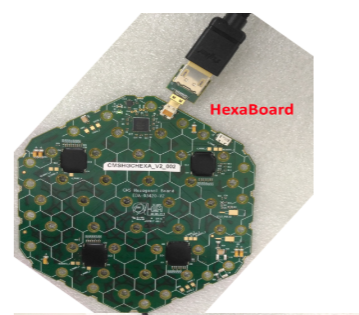
\includegraphics[width=0.45\textwidth]{PCB_study/Hexaboard.png}
     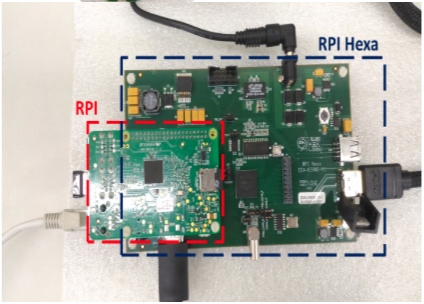
\includegraphics[width=0.45\textwidth]{PCB_study/RPI.png}\\
     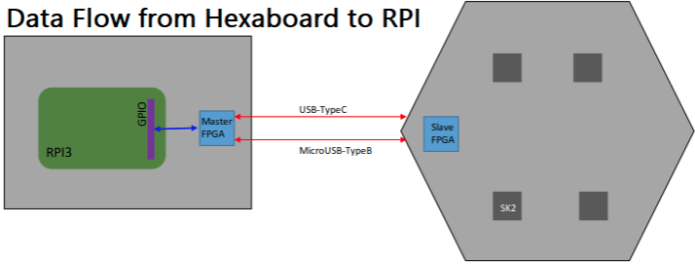
\includegraphics[width=0.9\textwidth]{PCB_study/Data_flow.png}
\caption{(Top left) The Hexaboard which was applied in the study. On the board, there are four SKIROC2cms CHIPs (black hexagonal) used to receive the electrical pulse which is given by the cable, and give out the signal to the Hexa RPI. (Top right) The Hexa RPI and RPI which is applied to transform the data and communicate with Hexaboard. (Down) The data flow pictures for introducing the data transfom from Hexaboard to Hexa RPI and RPI.
}
\label{fig:PCB_study_apparatus}
\end{figure}

Every SKIROC2cms CHIP on the HexaBoard corresponds to 64 channels, while each channel has its own readout circuit(Pre-amplifier, shapers,etc.). In each event(run), it recorded 30 numbers to reconstruct the event for every channel. Totally 30 numbers are given by 13 ADC counts in both highgain(HG) and lowgain(LG) plus 2 TOTgain(Time Over Threshold) and 2 TOAs(Time Of Arrival).  The 13 ADC counts of HG and LG come from 13 SCA(Switched Capacitor Array) units in the circuit, which sample the input signal every 25ns\footnote{There exist thirteen different capacitors with the number SCA0, SCA1....SCA12, and they will record one ADC value in order every 25ns for the each channel of CHIPs. When going to SCA12 and finishing recording, it will return to SCA0. The order of SCA numbers are not related to the order of the electrical pulse we give, but the time stamps are.}. They can be used to define the hardware noise and differences between each capacitor. At the same time, we recorded the time stamp with the pulse trigger\footnote{In real case, it recorded the starting SCA and the end of SCA with roll position array when the pulse trigger is on and off, and rearrange the SCAs with this array as the time stamp, so it can be specified as the pulse information.} for each event. Time stamp label the whole pulse in order,  so we can use the time stamp to mark the pulse location, specially for the peak of pulse. 

\subsection{Events and Methods for analysis}

For simplifying the study, we used the Hexaboard without the sensor on it. In this studies, we used two types of runs to do the researches through the whole process:
\begin{itemize}
\item Pedestal run: Run without injecting the electrical pulse, and record the non-pulse run to be our reference.
\item Charged run: Run with injecting the electrical pulse to the certain channel, and record the with-pulse run to do the study. 
\end{itemize}

Be attention with, because we simulated the sensor-attached condition, and sensor only apply the 32 channels on the Hexaboard in real life, we used 32 channels of the Hexaboard to study. In the Fig.\ref{fig:PCB_study_channelMap} is the channel map that we used in the study.

\begin{figure}[!htb]
\centering
     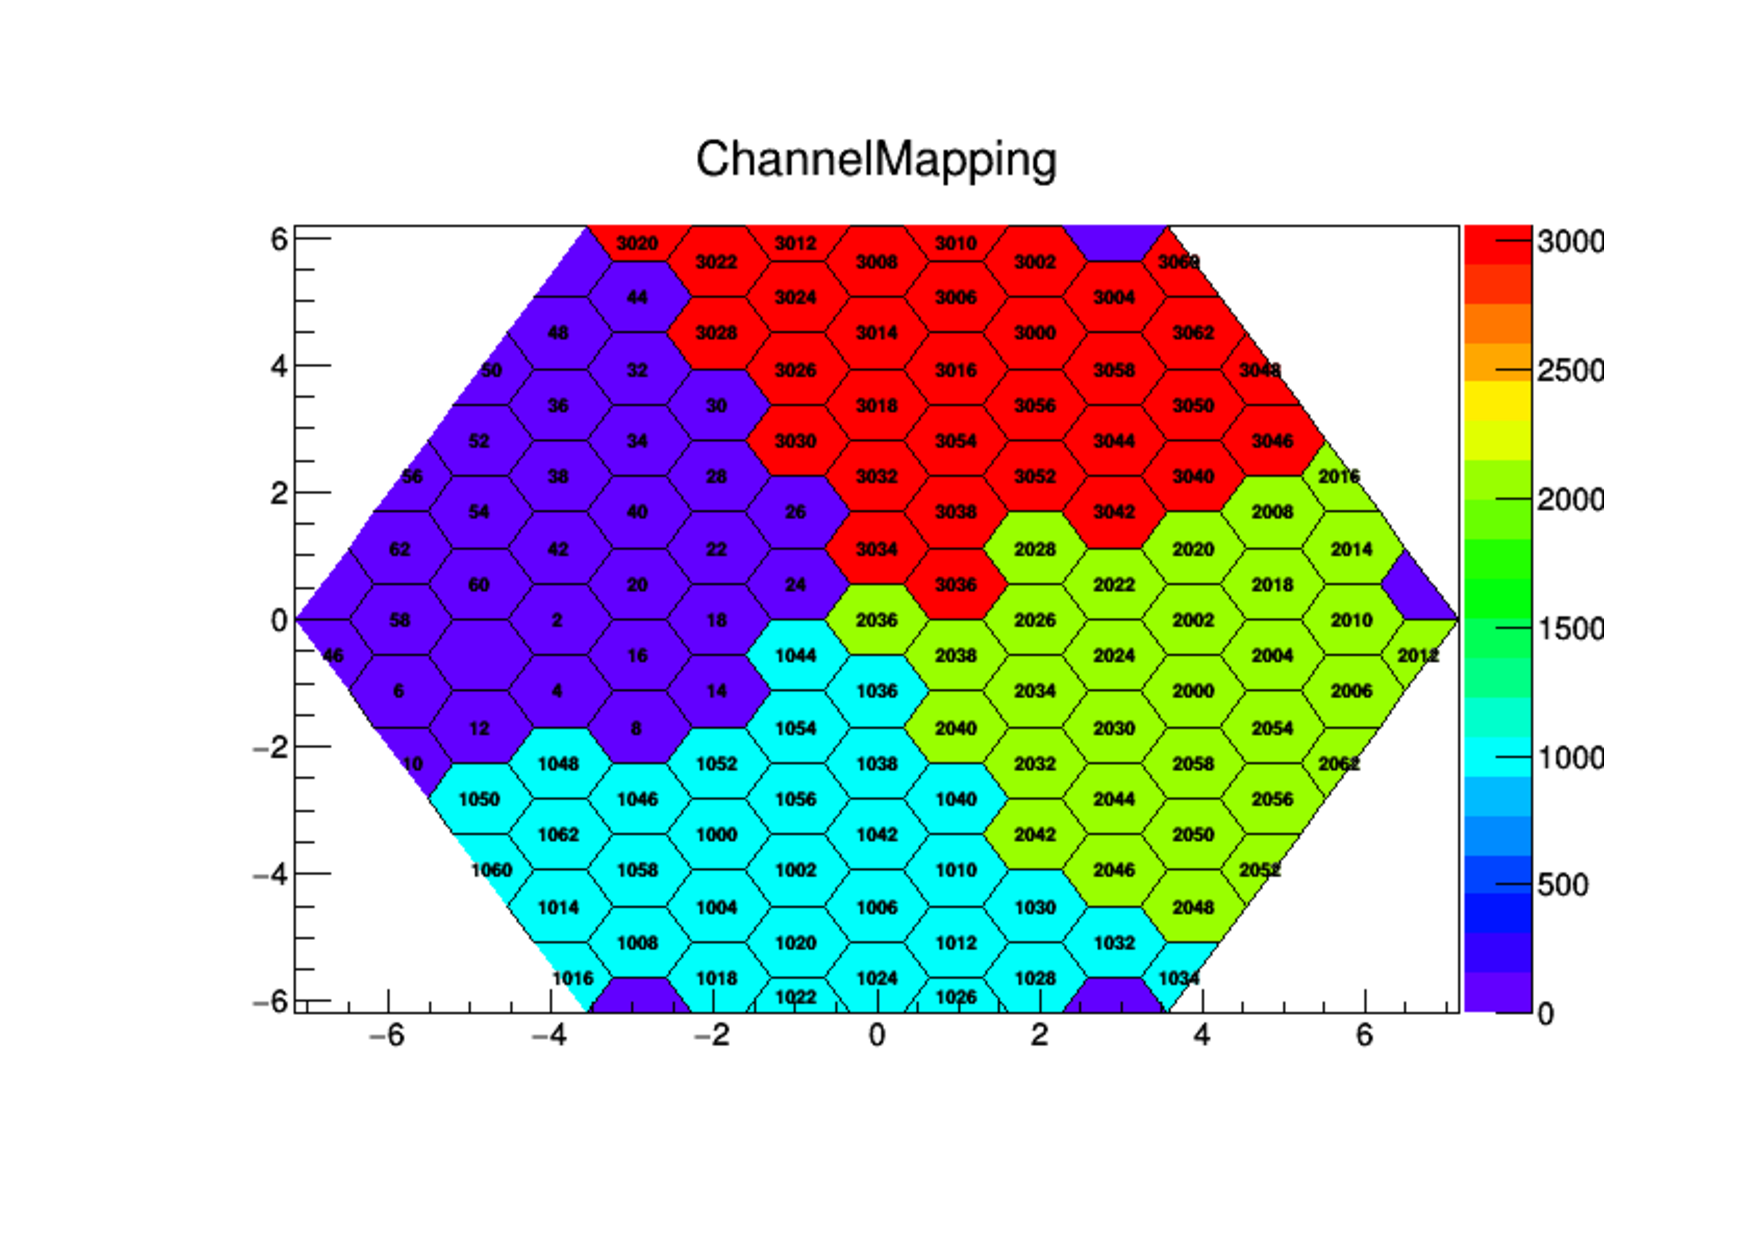
\includegraphics[width=0.9\textwidth]{PCB_study/channelmap.pdf}
\caption{The channel map which was applied in the research, there are four regions with the different color represent the different SKIROC2cms CHIPs.  A digit in thousands is the order of the CHIPs, and a digit in tens and ones represent the channels on each CHIPs.}
\label{fig:PCB_study_channelMap}
\end{figure}

The following three cases which were used in our studies are shown in the fig.\ref{fig:PCB_His}. (1)Pedestal run were used to evaluate the pedestals and noise for each channel. The value of mean of ADC-counts will be defined as the pedestal value from each channel, and it is the hardware-dependent(SCA-dependent) value. (2)Charged run were used to record the responses with ADC-counts values from every channel with the electrical pulse injecting, and simulated the real physics. (3)In the end, the "Pedestal-subtracted" value will be used in our study for subtracting the "reference". The mean value of the ADC-counts for it is calculated after Charged run ADC-counts subtract the mean of ADC-counts from Pedestal run with same SCA number. And the error( width of gaussian ) means the noise in the channels including the electronics noise, sensor noise( if it is installed ), etc. Note, in the study, we always used SCAs of HG to do. For simplifying the case, we fixed the injected-channel to number 20 in CHIP 0 and saw all cases.

\begin{figure}[!htb]
\centering
     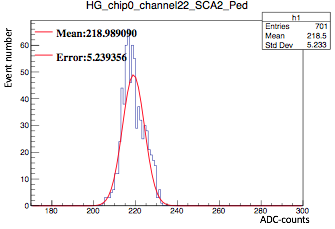
\includegraphics[width=\cmsFigWidth]{PCB_study/His_Pedestal.png}
     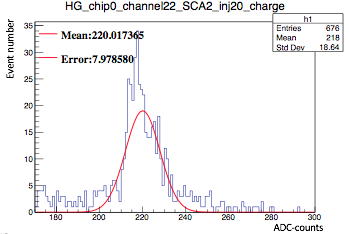
\includegraphics[width=\cmsFigWidth]{PCB_study/His_charge.png}\\
     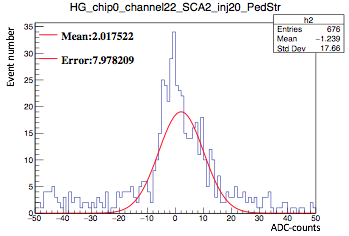
\includegraphics[width=\cmsFigWidth]{PCB_study/His_subtraction.png}
\caption{These figures perform the histograms that using in the study. All this cases are shown with fixing at SCA=2 and channel=22. (Top left ) The pedestal run histograms which is used to calculate the pedestal and noise. Fitting the line is to get the mean of ADC-counts. (Top right)  The charged run for example. (Down) The pedestal-subtracted case is shown. Also fit the line to get the mean and error of ADC-counts, and use in the study directly}
\label{fig:PCB_His}
\end{figure}

\subsection{Results and Conclusion}
First of all, because the first SCA (the 0th) is useful for making on-line pedestal subtraction (because there may be some low frequency noise), and usually our signal comes after SCA0, we need to explore the correlation between the stability of pedestals(SCA0) and other SCA sampling.  In the Fig.\ref{fig:PCB_Stability}, we can see that the nearest channel of the injection channel (channel 20) with channel 18 and 22 as examples, the stability of them are very good. Because the fitting lines are pretty flat in both of them, and that means in the different SCA number other than SCA0, they are slightly different. And we can see the same condition in other channels also.

\begin{figure}[!htb]
\centering
     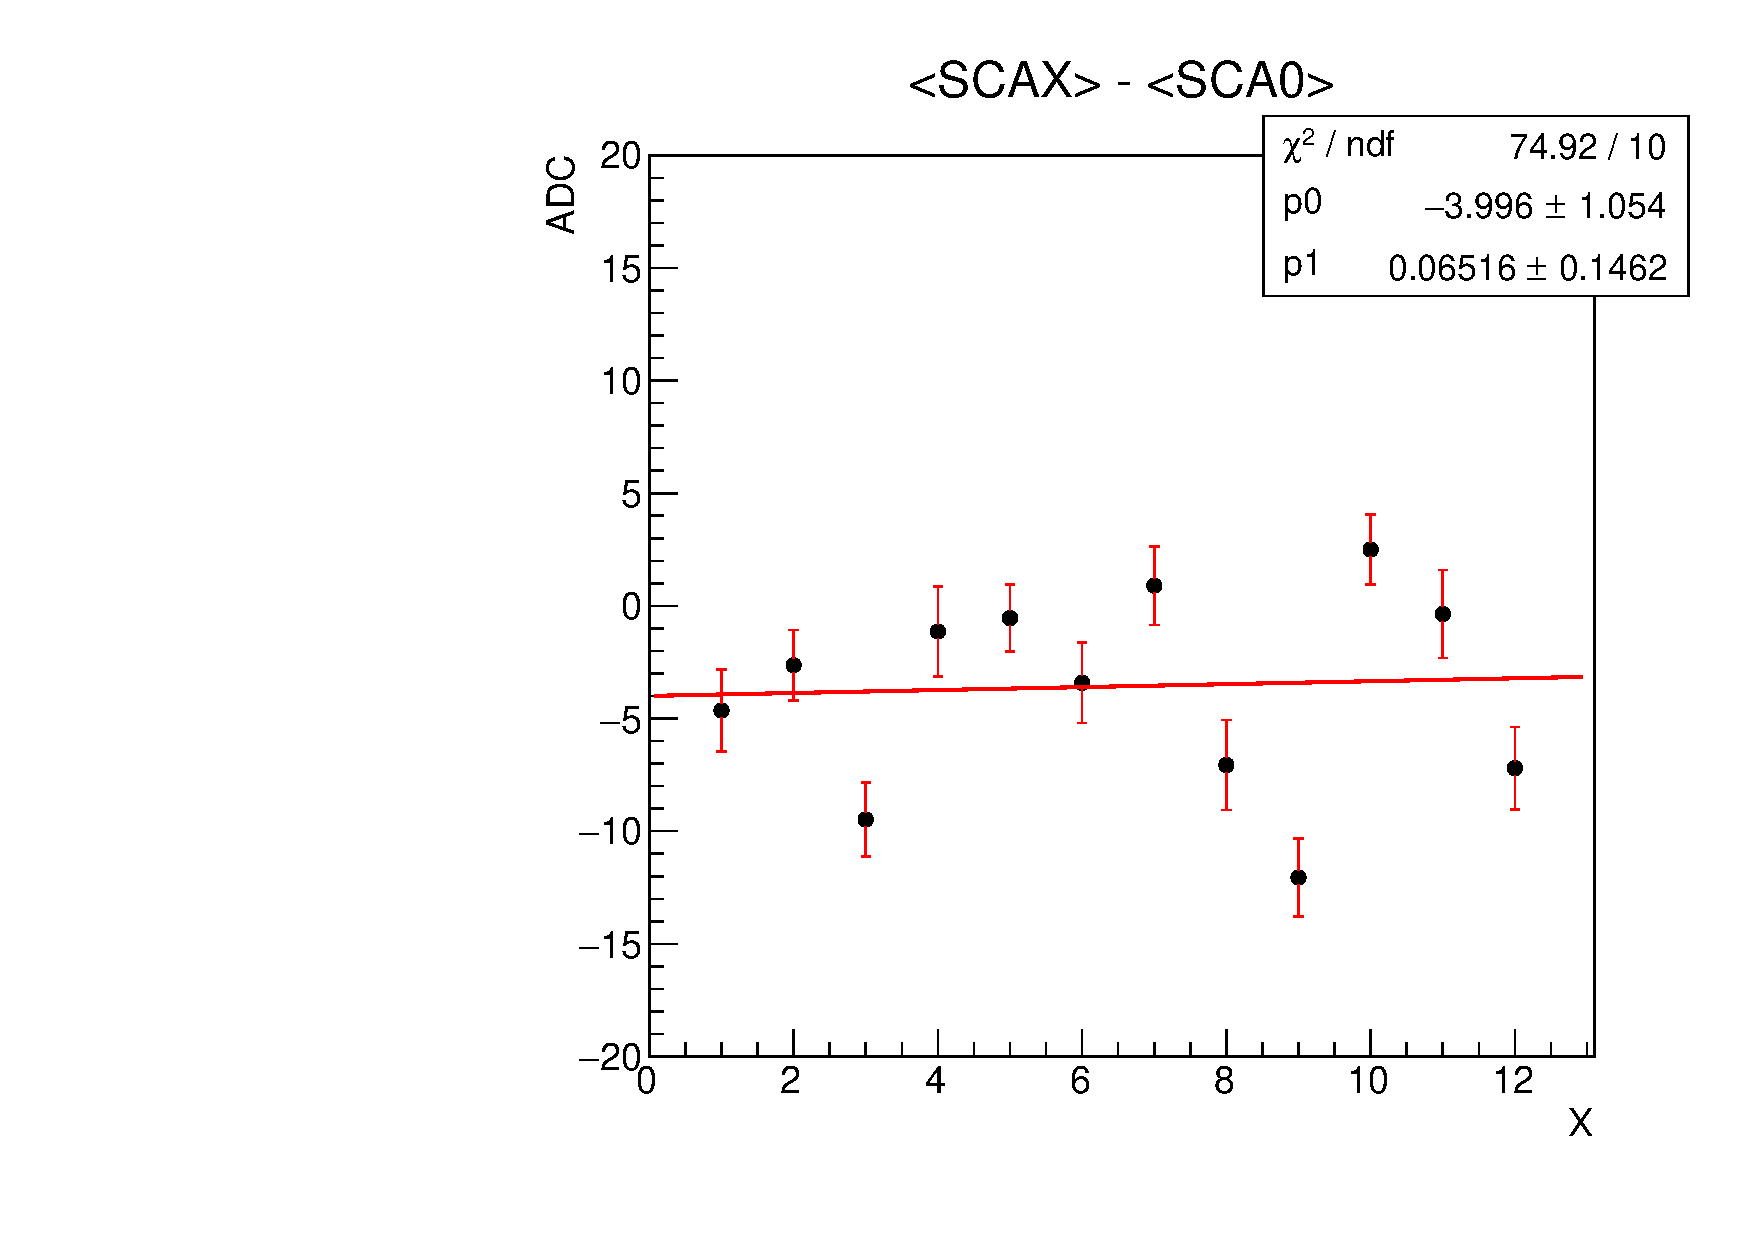
\includegraphics[width=\cmsFigWidth]{PCB_study/HG_Chip0_channel18_Subtract_mean_Stability.pdf}
     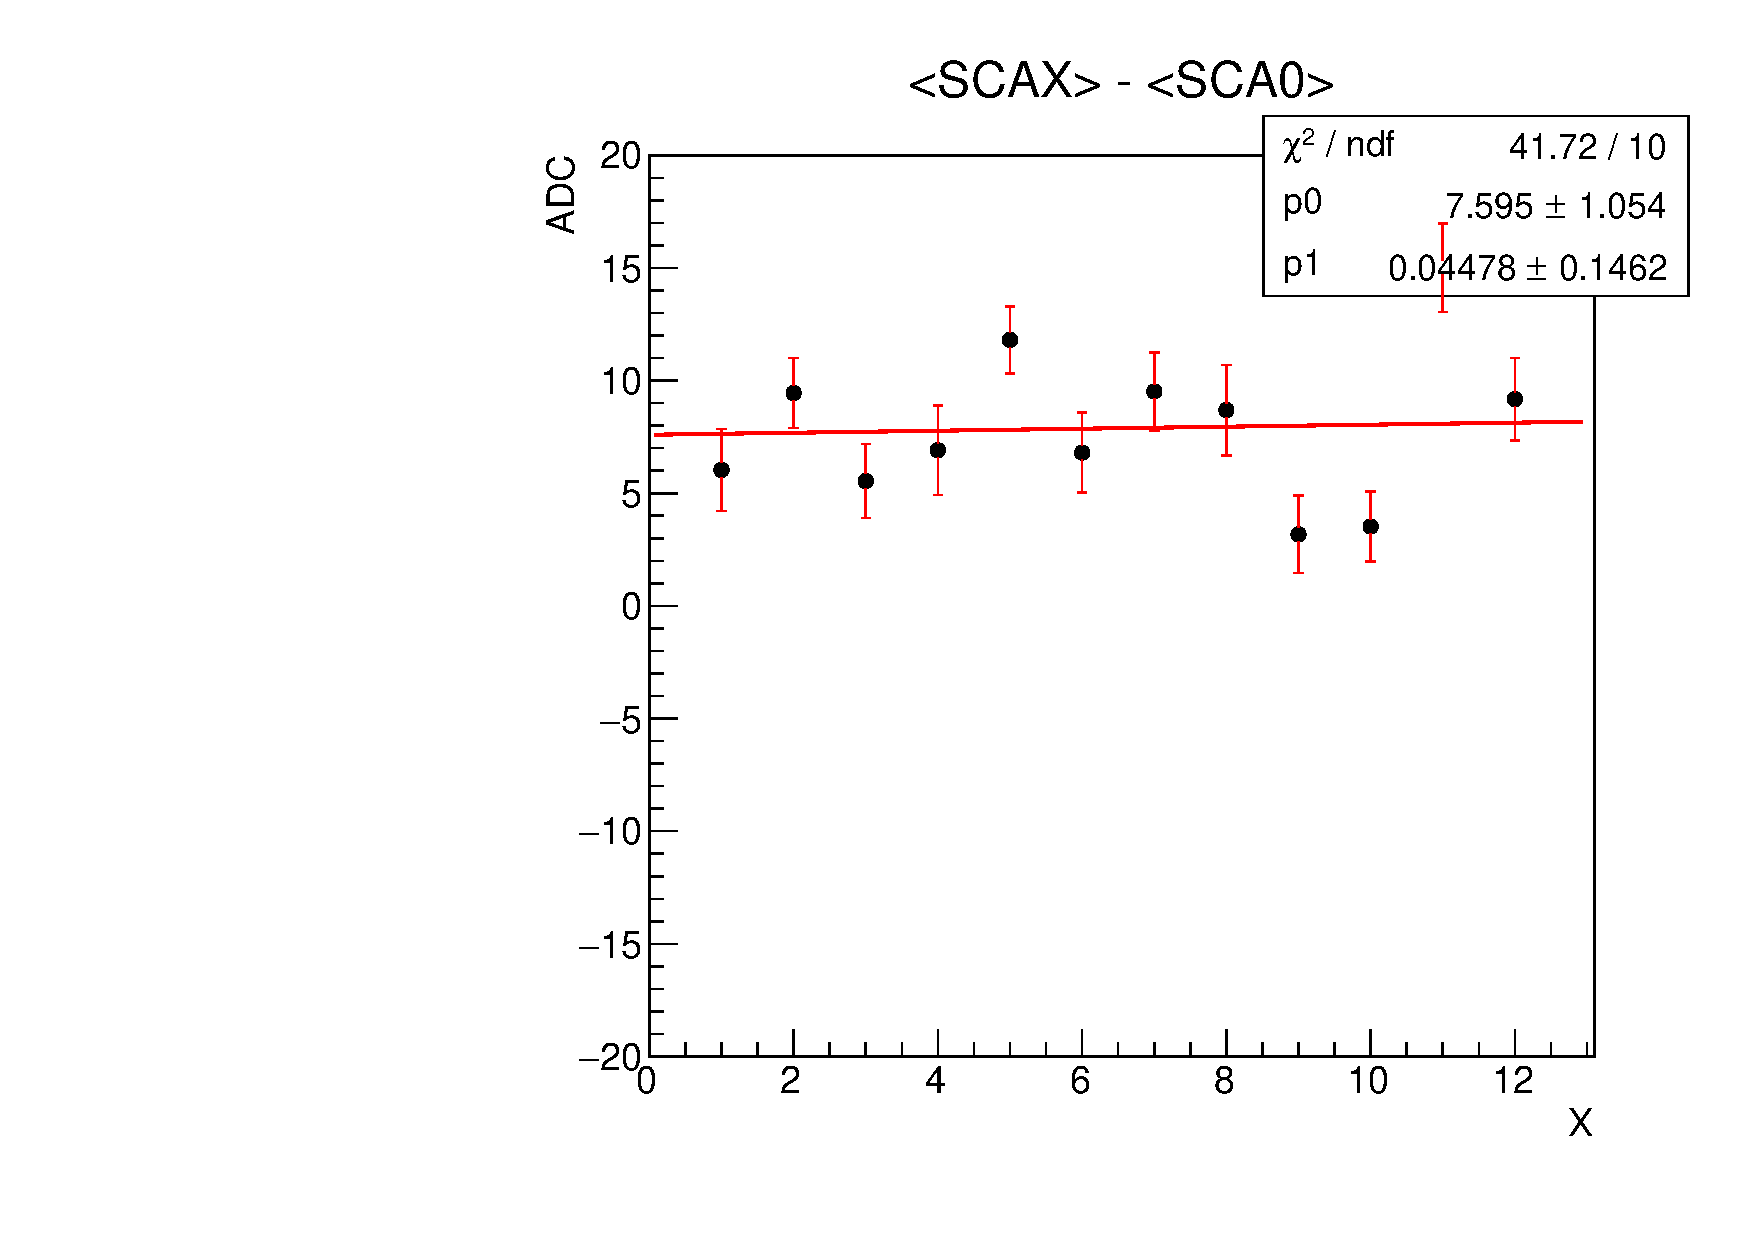
\includegraphics[width=\cmsFigWidth]{PCB_study/HG_Chip0_channel22_Subtract_mean_Stability.pdf}\\
\caption{The figures show the difference mean of ADC-counts between the first SCA and other SCAs. (Left) The channel 18 response and (Right) The channel 22 response.
}
\label{fig:PCB_Stability}
\end{figure}

Second, we wanted to explore the correlation between injection pulse strength and the cross-talk. In real physics, because particles will have different energy individually in the collider, they will see the different pulse strength in the real case. At there, we wanted to see whether the different pulse strength will give out more or less the cross-talk. In the fig.\ref{fig:PCB_injection_pulse_study}, they show that the mean and error values from Pedestal-subtracted value for different DAC of injection pulse. The results for them are quiet obviously showing that the cross-talk in two cases: 
\begin{itemize}
\item Anti-correlated cross-talk\\
DAC from 0 to 1000: No matter the closer or farther the channels, the slopes are negative for all of them. That means the channels, except the injection channels, are borrowed the energy by injection channels. 
\item Correlated cross-talk\\
DAC after 1000: When the channels are closed to the injection channels, the slopes are bigger compared with the channels which are farther from the injection channels. That means, the injection channels give more energy to the closed channels compared with the farther channels. 
\end{itemize}

\begin{figure}[!htb]
\centering
     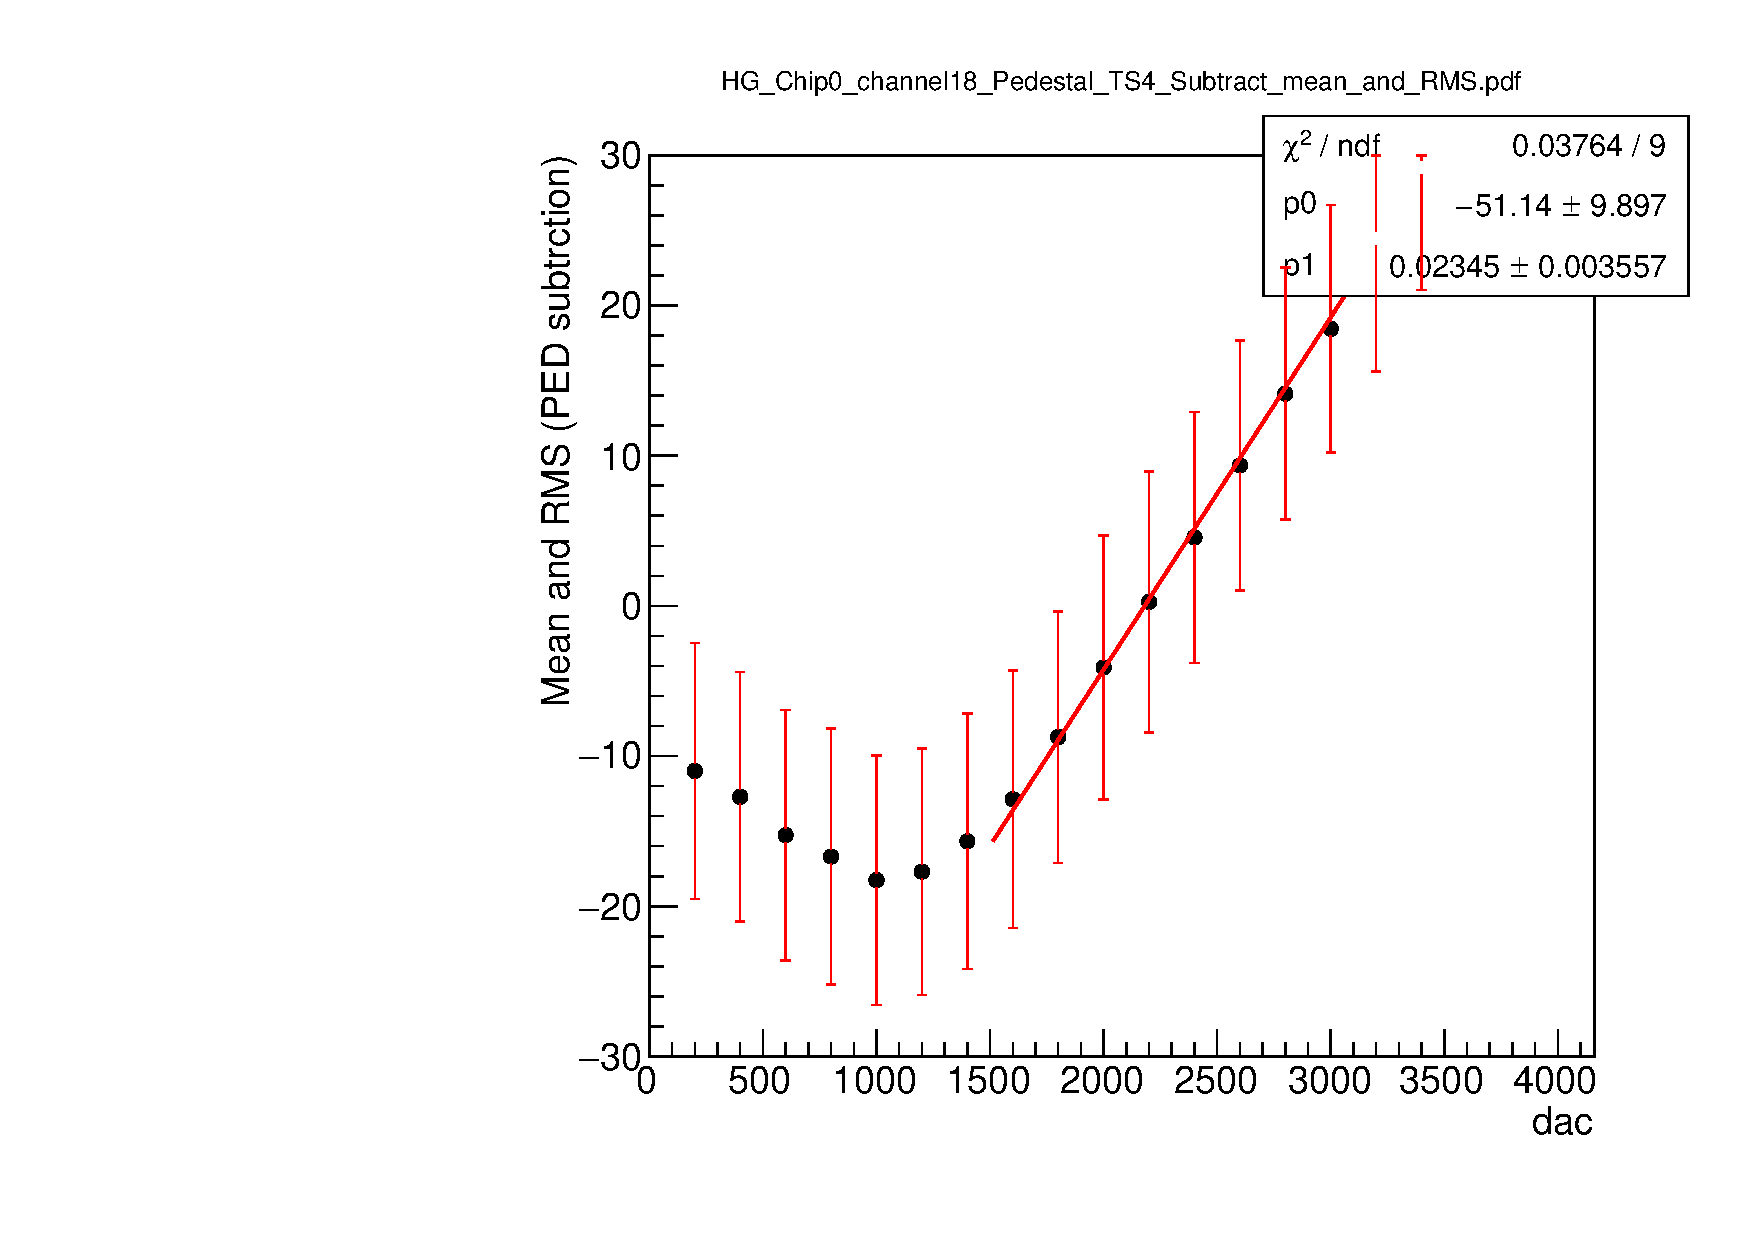
\includegraphics[width=\cmsFigWidth]{PCB_study/HG_Chip0_channel18_Pedestal_TS4_Subtract_mean_and_RMS.pdf}
     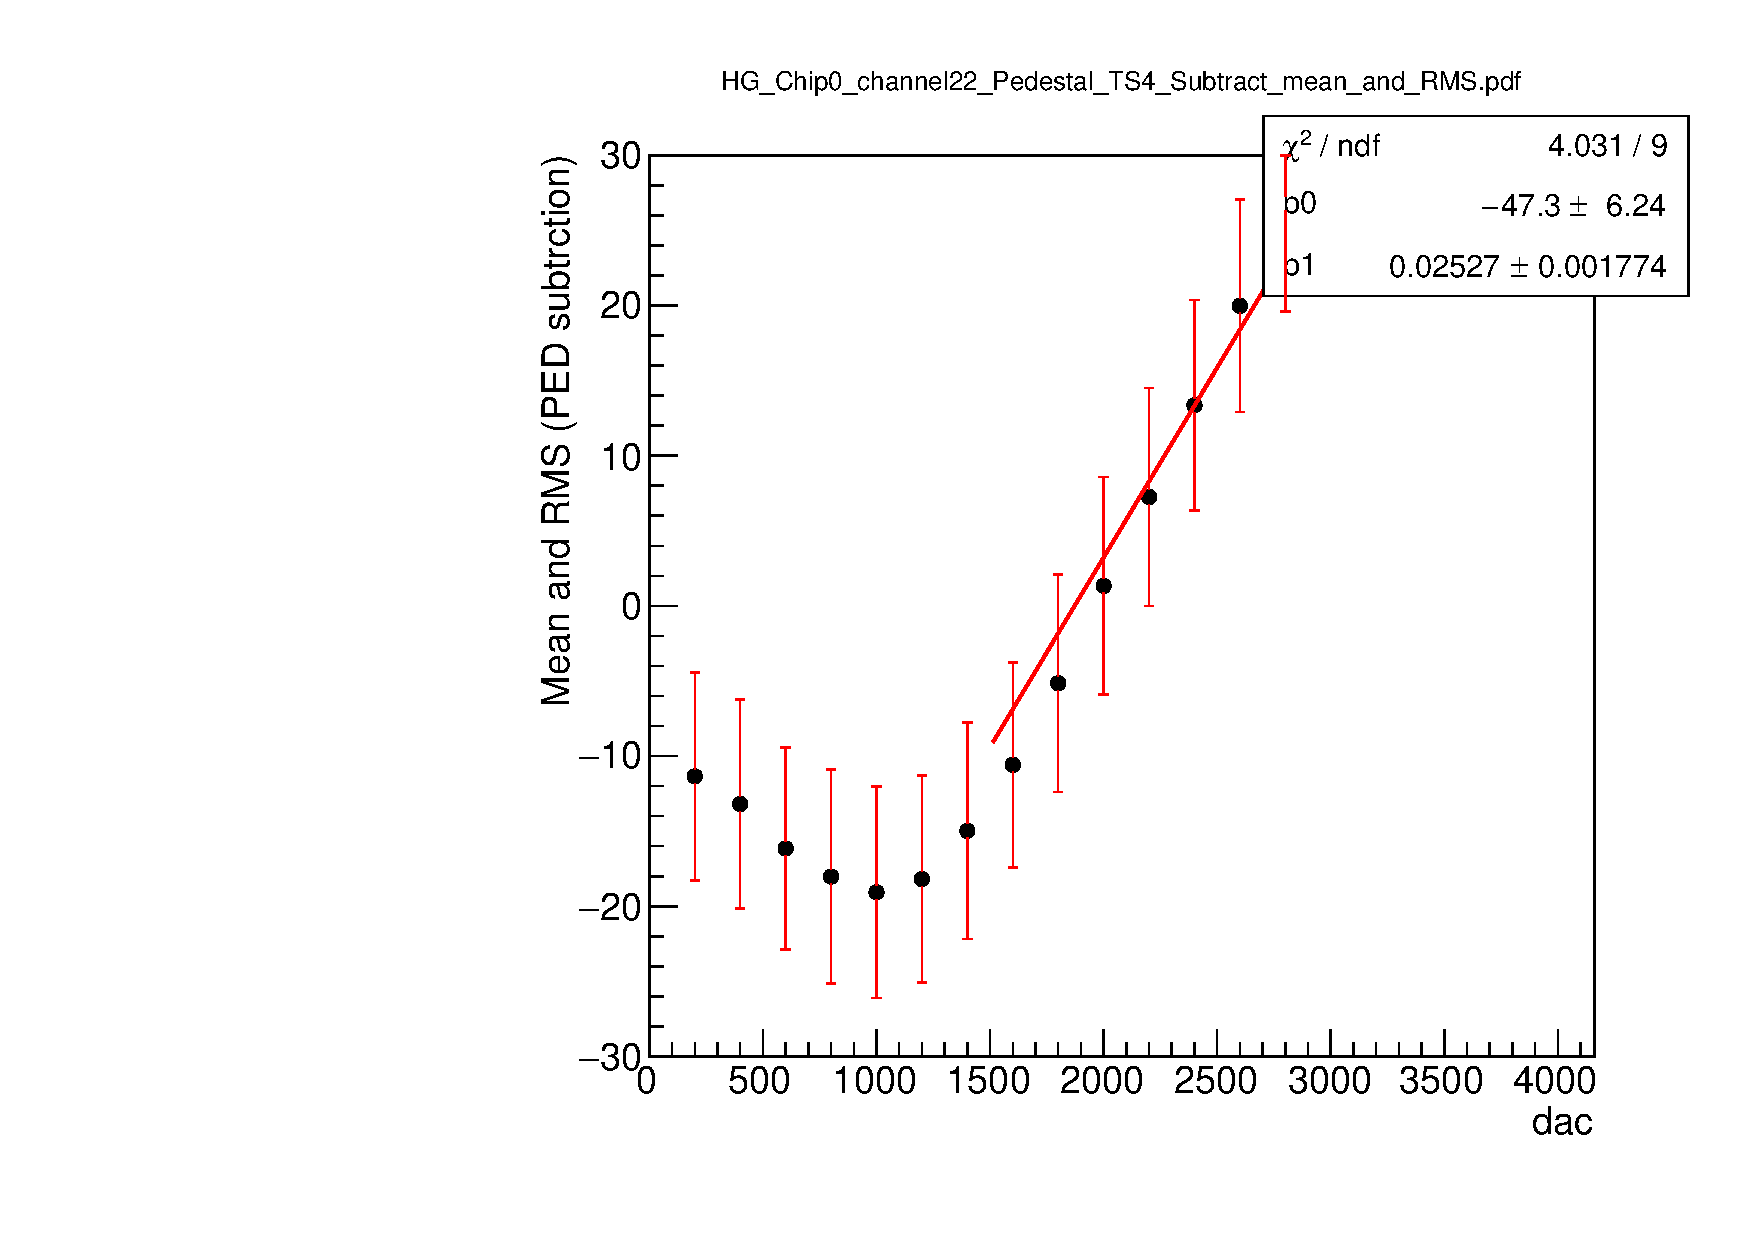
\includegraphics[width=\cmsFigWidth]{PCB_study/HG_Chip0_channel22_Pedestal_TS4_Subtract_mean_and_RMS.pdf}\\
     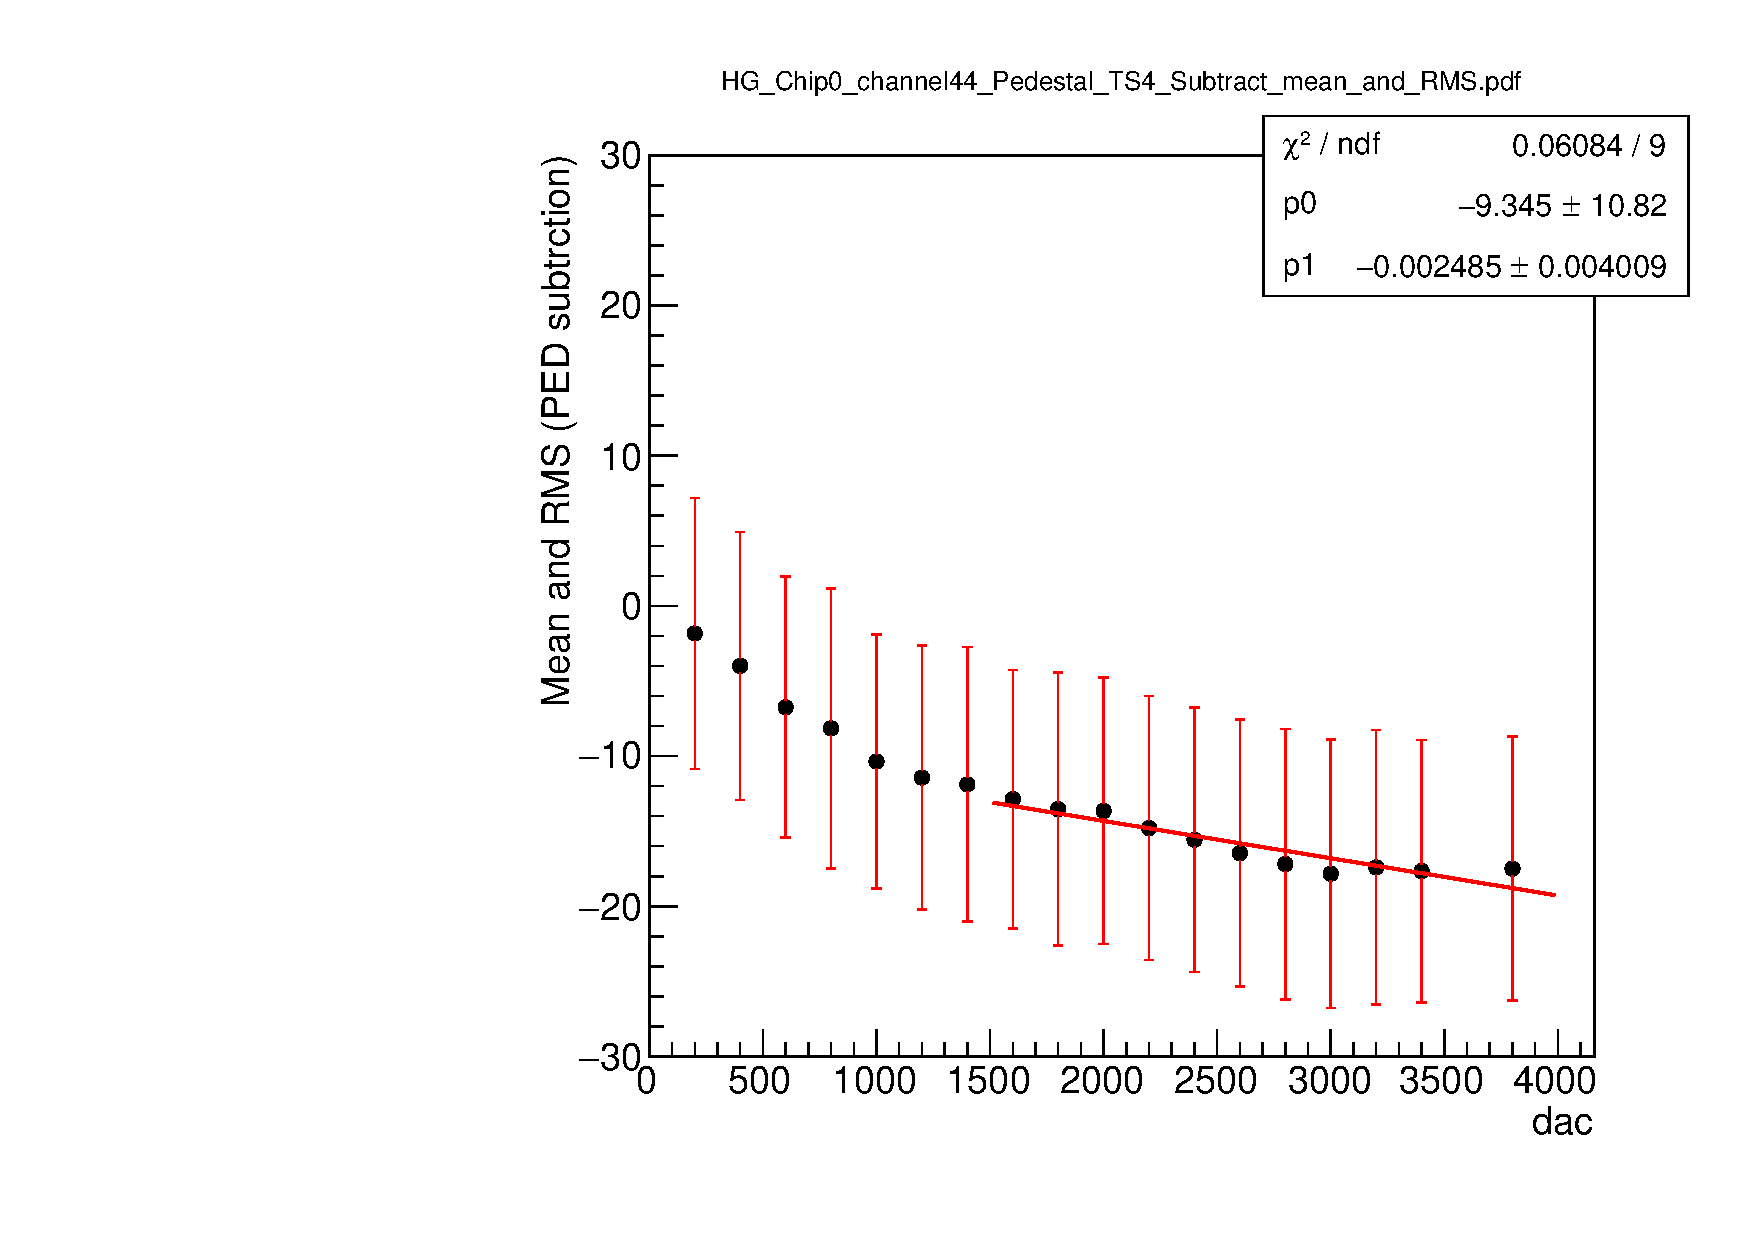
\includegraphics[width=\cmsFigWidth]{PCB_study/HG_Chip0_channel44_Pedestal_TS4_Subtract_mean_and_RMS.pdf}
     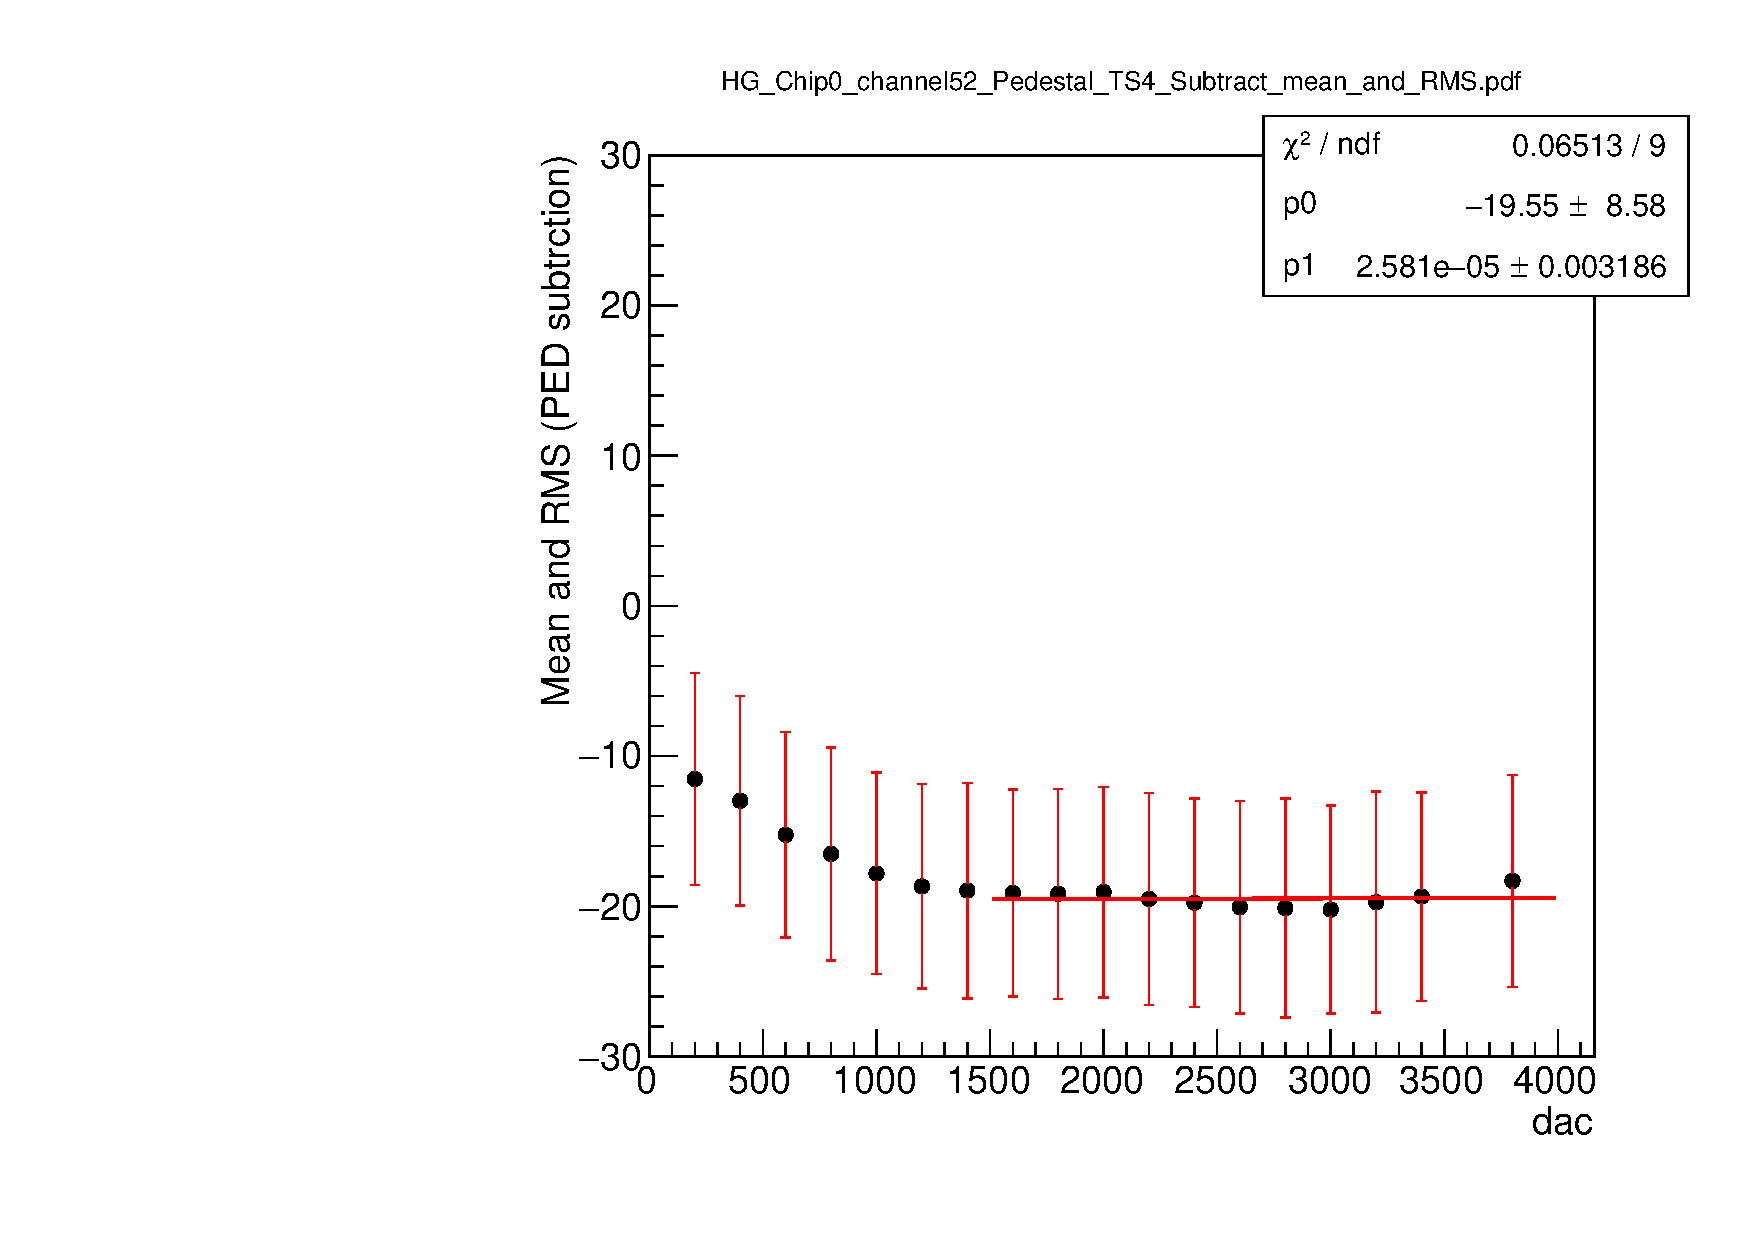
\includegraphics[width=\cmsFigWidth]{PCB_study/HG_Chip0_channel52_Pedestal_TS4_Subtract_mean_and_RMS.pdf}
\caption{These figures present the preliminary results for the correlation between the different DAQ input and Pedestal-subtracted mean and error. The Top left and right pictures perform the channel of 18 and 22, which are closed to the injection channel. The down left and right pictures show channel of 44 and 52, which are farther from the injection channel.}
\label{fig:PCB_injection_pulse_study}
\end{figure}

For the conclusion, we can see from our study that the cross-talk exist in the Hexaboard, and we used the ADC-counts from the Pedestal-subtracted values to quantify the cross-talk. We expected that this study can help to quantify the cross-talk and can decrease it in the future.

\section{Pion-rejection studies with a CMS HGCAL test-beam prototype ECAL}
In most cases, the electrons leave most of the energy in ECAL by the processes of pair production and bremsstrahlung. Different from them, Chagred-pions deposit most of the energy in Hadronic Calorimeter(HCAL) through the process of segmentation. Unfortunately, in some cases, those pions could give out the fully Electromagnetic(EM) showering in ECAL, and put most of the energy in it. If we can't explore the way to tag those pions and reject them, it will be very terrible. Because they will be misidentified as the electrons, and those "fake electrons" could contaminate with the real electrons.  In addition, it could influence the analysis which is sensitive to the electron/pion distinguishability. We expected to solve this issue and help the physics analysis with this type of background in the future.

Because of the significant challenges for radiation tolerance and event pileup on the detectors of the CMS experiment at LHC, they will replace the current Endcap calorimeter with a Si-pad HGCAL, a new generation state-of-the-art calorimeter, which can perform 3D imaging of the shower as well as provide ~30ps timing. To test the performance of HGCAL, including calibration, particle identification, etc. before it will be installed in CMS Phase \rom{2} upgrade , we did the "test-beam"(Fig.\ref{test_beam_setup_1}), which was held to incident the test particles, such as electron, pion and muon into HGCAL prototype, and analyze its performance from the information of the hits come out with the detector. At the same time,  The Monto Carlo(MC) samples are provided with the same prototype of the detectors to let the people study as well.  We used the test-beam MC samples which are done in CMS on June and October 2019 to do this study. The group of test-beam divided the studies into many different topics, and my topic was in the section of "electron/pion identification".
\begin{figure}[!htb]
\centering 
     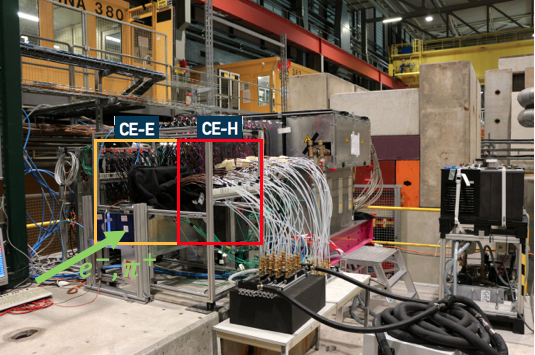
\includegraphics[width=0.9\textwidth]{Delta-ray/test-beam_setup.png}
\caption{The figure show the test beam experiment setup in October. The orange and red lines box mark the CE-E and CE-H part of the detector including the module(in the metal box) and readout electronics.}
\label{test_beam_setup_1}
\end{figure}

Charged-pion tagging and rejection are one of the strong points of HGCAL. Traditionally the most powerful discriminants for pion rejection are lateral shower containment and longitudinal energy leakage in the back of the EM section of HGCAL. In this study we explore the capability of HGCAL to tag pions that are fully EM-showering in the ECAL and they pass the transverse containment and leakage from the back requirements. For our expectation, we wanted to find the best cuts and invited the new variables to distinguish "fake electrons" from "real electrons".

I did this study with Prof. Stathes Paganis, Prof. Rong-Shayang Lu, master student Chia-Hong Chein from NTU, Dr. Shilpi Jain from University of Minnesota and Prof. Shin-Shan Eiko Yu from NCU.  The contributions of Chih-Hsiang Yeh to this study includes the following:
\begin{itemize}
\item Study the optimized cuts for finding the "fake electron" from pions, and introduce the new variable with the longitudinal segmentation using the test-beam MC samples from June.
\item Apply the found optimized cuts and new variable in test-beam MC samples from October to see the electron efficiencies and pion rejections.
\end{itemize}
I will describe the detail as following.

\subsection{Introduction for HGCAL}
During the Run 1 (2010-2012) in LHC operated at $\sqrt{s} = 7\TeV$, delivering $\approx$ 6\fbinv, and at $\sqrt{s} = 8\TeV$ in 2012, delivering $\approx$ 23\fbinv. The most significant physics results from this period was the discovery of the Higgs boson, and along with the Nobel prize for it in 2013. After Run 1, Run 2 started in 2015 at a C.M of $\sqrt{s} = 13\TeV$  and the instantaneous luminosity, reaching to the value for $1.7 \times 10^{34} cm^{-2} s^{-1}$. In the Figure.\ref{luminosity_1}, it shows the summary plot for the luminosity from Run1 to Run2.  Surprisingly, it operated the exceed value compare with the original design. More studies with this unbelievable operation, such as Higgs boson, SM processes, BSM, will be carried out.

\begin{figure}[!htb]
\centering 
     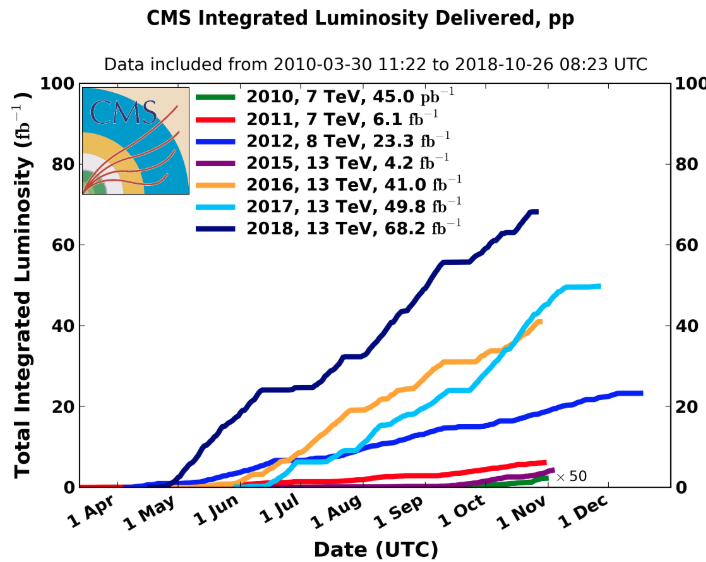
\includegraphics[width=\cmsFigWidth]{Delta-ray/Luminosity.png}
     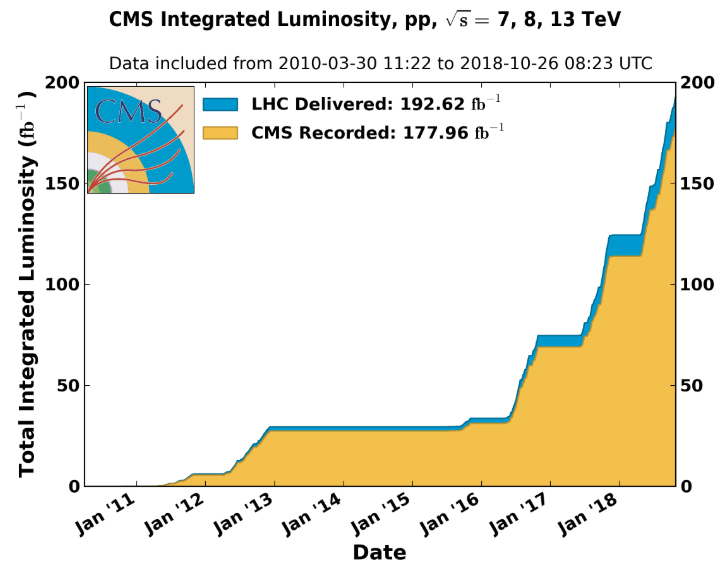
\includegraphics[width=\cmsFigWidth]{Delta-ray/Luminosity_total.png}
\caption{The figures show the summary plot of luminosity from the Run1(2010-2012) to Run2(2012 to 2018) in LHC. The left is the luminosity for the individual years, and the right is the totally integrated luminosity from 2010 to 2018.}
\label{luminosity_1}
\end{figure}

For the future in Run3(2023), LHC intended to accumulate around 300\fbinv. After the third long shutdown (LS3), they plan to design the value to the instantaneous luminosity at $5 \times 10^{34} cm^{-2} s^{-1}$ with the target of integrating around 3000\fbinv by the time of mid-2030s, and it will go into the HL-LHC era. The corresponding mean number of collisions (pileup) per bunch crossing will be 140. In addition, the LHC has the ability to deliver 50\% higher values for both the instantaneous and integrated luminosities.

In this case, It will bring out the two significant issues in the HL-LHC era: (1)radiation damage and (2)event pileup on CMS detectors, especially for calorimetry in the forward region. As part of its HL-LHC upgrade program, the CMS Collaboration is proposing to build a HGCAL to replace the existing endcap calorimeters. There are many requirements for the HGCAL upgrade to let it preserve the good performance. Write some of them as following:
\begin{itemize}
\item  This detector must be "radiation tolerance", otherwise, it will happen the unrecoverable condition, same as the circumstance of scintillator now in CMS. To solve this issue, active layer with the silicon sensor will be applied in the HGCAL.
\item  This detector need to be designed with the find granularity for lateral and longitudinal segmentation:
\begin{itemize}
\item For the lateral part, it can help with separating two showers and can observe the narrow jets. 
\item For the longitudinal part, it can help us to probe the longitudinal development of showers, providing good energy resolution, and also can know more about the patterns in the physics processes.
\end{itemize}
Both of them can remove the "pileup event" if they are great enough to distinguish processes of different particles.
\end{itemize}

The HGCAL prototype consists of an electromagnetic compartment (CE-E) followed by a hadronic compartment (CE-H) with Forward region(FH) and Backward region(BH) in the Fig.\ref{HGCAL_region}. For the CE-E, it consists of 28 sampling layers with a depth of approximately 26 $X_{0}$ and 1.7 $\lambda$. In the Fig.\ref{HGCAL_Material} top left shows one sampling layer of the CE-E. The element of active layer for it is a hexagonal silicon sensor, which is sandwiched between layer of WCu (75\%, 25\%) baseplate and a printed circuit board(PCB), which is used to study my cross-talk studies in NTU, that carries the front-end electronics to form a silicon module in the Fig.\ref{HGCAL_Material} top right. Modules are tiled on a Cu cooling plate, which together with the two WCu baseplates form one absorber layer. The alternate absorber layer is formed by lead planes clad with stainless steel (SS) sheets that are placed on module-cooling plate sandwich. 

\begin{figure}[!htb]
\centering 
     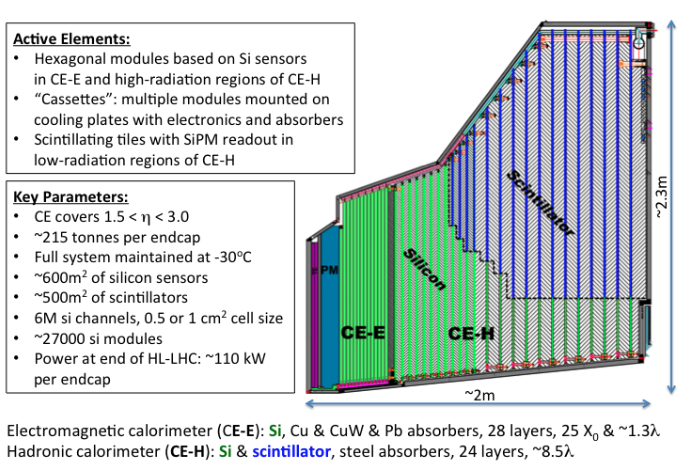
\includegraphics[width=0.8\textwidth]{Delta-ray/HGCAL_region.png}
\caption{Summary for the basic design and coverage of the CMS high-granularity Endcap Calorimeter (CE) including CE-E and CE-H}
\label{HGCAL_region}
\end{figure}

For the hadronic compartment of HGCAL, they consist of 12 planes of thick SS plates followed by another 12 SS planes with different thickness. Between these absorber plates sit silicon modules(show one sampling layer in Fig.\ref{HGCAL_Material} down left) in most regions and silicon modules mixed with scintillator tileboards(show one sampling layer in Fig.\ref{HGCAL_Material} down left) in part of low-radiation regions mounted on a copper cooling plates to form the wide cassettes.  These cassettes are similar to those in the EM compartment, but include sensors on only one side of the cooling plate, which are formed as a separate mechanical structure. This leads to a total interaction length with number 10.7$\lambda$, including the CE-E and the neutron moderator layer in front of the calorimeter. All layers are read out for use in energy measurement, but only alternate layers in CE-E, and all in CE-H, are used for producing L1 trigger primitives. 

\begin{figure}[!htb]
\centering  
     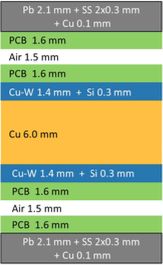
\includegraphics[height=\cmsFigWidth,width=\cmsFigWidth]{Delta-ray/CE-E.png}
     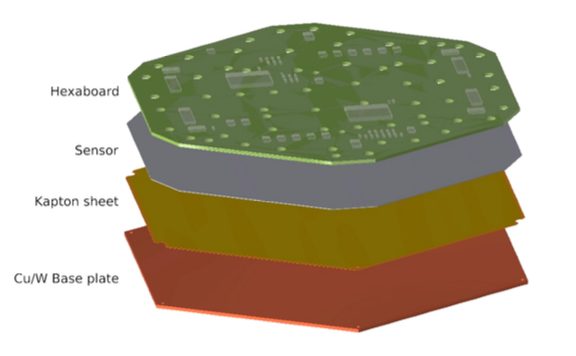
\includegraphics[height=\cmsFigWidth,width=\cmsFigWidth]{Delta-ray/Silicon_module.png}
     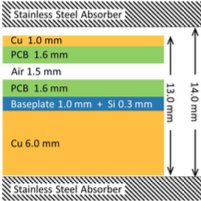
\includegraphics[width=\cmsFigWidth]{Delta-ray/CE-H(part1).png}
     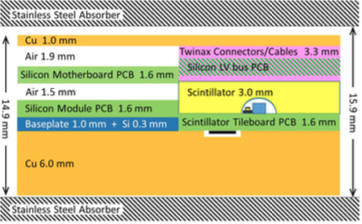
\includegraphics[height=\cmsFigWidth,width=\cmsFigWidth]{Delta-ray/CE-H(part2).png}
\caption{The figures show the different material arrangement in the different part of the detector. The top left is the one sampling layer of the CE-E. The top right show the silicon module used in the CE-E and CE-H. The down left is the one sampling layer of the CE-H which is sit on the high-radiation region. Oppositely, the down right is the one sampling layer of the CE-H which is based on the place with low-radiation.}
\label{HGCAL_Material}
\end{figure}

In the test-beam, we used the material based on prototype of HGCAL written below,  but for the detail of its, each components will use the CMS phase 2 design. I will write the results of the test-beam in 2018 on June and October.  

\subsection{Tag-and-probe the optimized cuts and new variable with June test-beam MC}
Because we wanted to tag the "electron-like"(e-like) pion, we need to explore the properties for the electron first, including shower shape, energy deposition, etc. in detector. And then, apply all of them in pion runs to tag those bad pion. I will describe the detail for the cuts and selections as following. In this studies, we used the sample with 50GeV electron and pion MC.

\begin{figure}[!htb]
\centering
     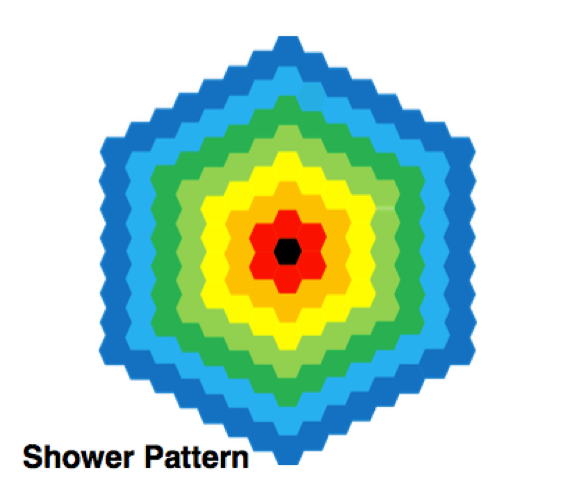
\includegraphics[width=\cmsFigWidth]{Delta-ray/Shower_pattern.png}
     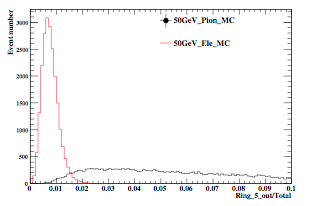
\includegraphics[width=\cmsFigWidth]{Delta-ray/5-Rings_cuts.png}\\
     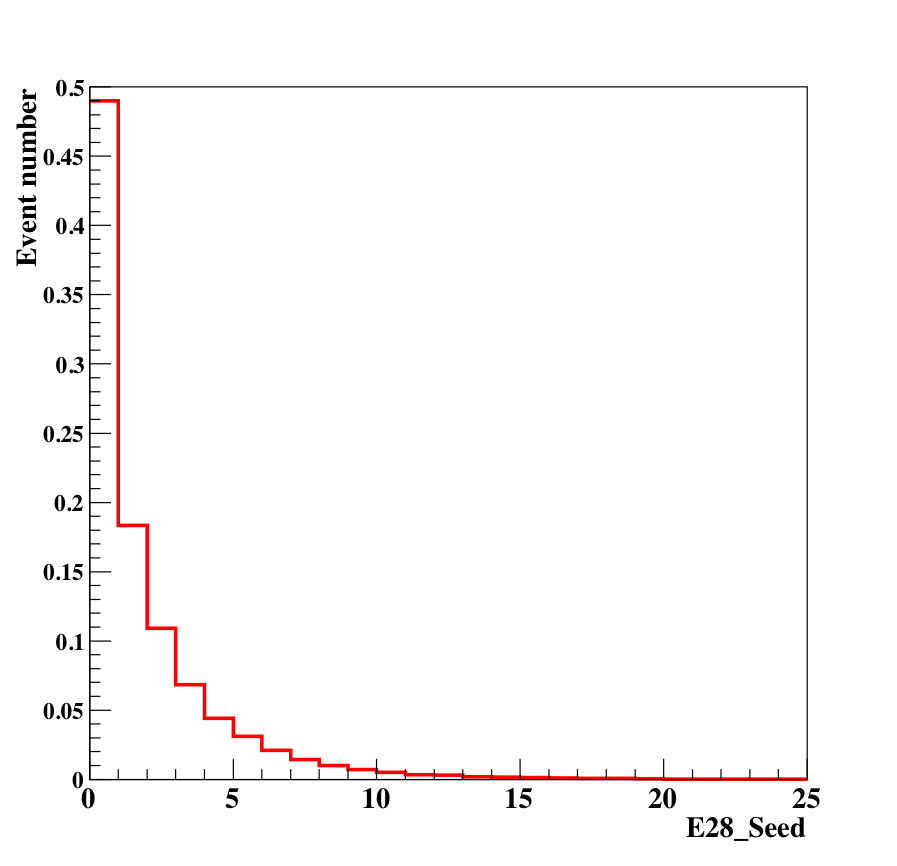
\includegraphics[width=\cmsFigWidth]{Delta-ray/Last_layer_20MIPs_50GeV.png}
     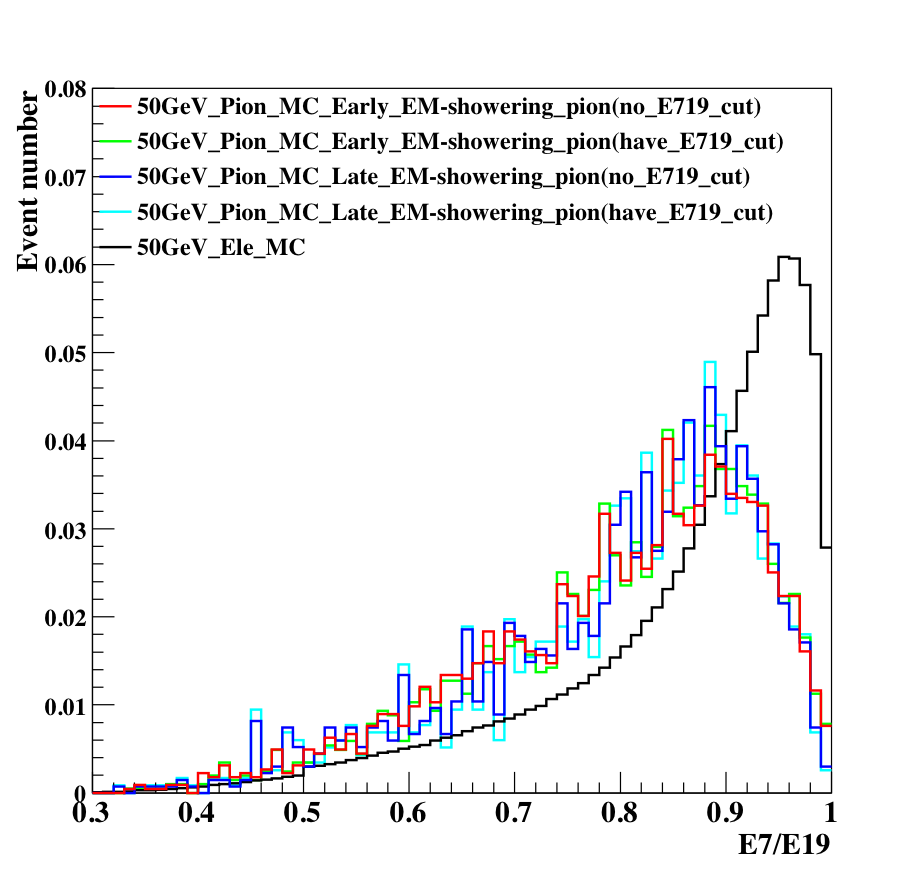
\includegraphics[width=\cmsFigWidth]{Delta-ray/E7_E19.png}
\caption{These figures present the cuts we used in the studies. Top left is the shower pattern on the transverse plane in the detector. Different rings mean the different sizes of the clustering on it. For example, the 5-Rings means the fifth circle calculated from the black pad to the shadow green. The top right plot is the energy distribution of $\frac{\mathrm{energy \ out \ of \ the \ 5 \ Rings}}{\mathrm{total \ energy}}$. The down left is the last layer energy with electrons. The down right is the cut with $\frac{\mathrm{energy \ in \ 2 \ Rings}}{\mathrm{energy \ in \ 3 \ Rings}}$, we plot every layer $\frac{\mathrm{energy \ in \ 2 \ Rings}}{\mathrm{energy \ in \ 3 \ Rings}}$ value with and without the $\frac{\mathrm{E_{7}}}{\mathrm{E_{19}}}$ cut}
\label{cuts_1}
\end{figure}

The first selection, because electron and pion have very different shower shape(width) on the transverse plane in ECAL, we studied on them at starting. From the theory, it tells us that electron has the narrower shower shape than pion in ECAL, we explored the cut with the different number of rings on the transverse plane of detector. In the Fig.\ref{cuts_1} top left shows the distribution plot of ring. In the end, we chose the energy of 5 Rings for being the cuts. Fig.\ref{cuts_1} top right is presented to show the cut we used with "$\frac{\mathrm{energy \ out \ of \ the \ 5 \ Rings}}{\mathrm{total \ energy}}$". Because we can see in the plot, the energy of electrons showering are collected out of the 5 Rings with at most 1\% compared with total energy in ECAL.  We chose this standard to tag the e-like pions first. Although, it is the tight cut because it also discarded some of electrons as well, but we wanted to make sure that we cut-off the bad pion really. We called this cut as "5-Rings cut".

The second selection, because we wanted to select the "fully EM-showering", and we didn't have the information of HCAL energy in this month test-beam, we only could use the "poor man's solution"-finding the last layer energy of electrons and using it to be our cut. In the Fig.\ref{cuts_1} down left is the plot which was used to find the cut of last layer energy with the events which passed 5-Rings cut . Eventually, we used the last layer energy smaller than 20MIPs to tag the fully showering events, we called this cut as "The last layer energy cut".

The third selection, it was the cut always used to find the EM-showering in pion traditionally, and related to the shower shape also, similar with the first selection. In every run, we applied the cut with "$\frac{\mathrm{energy \ in \ two \ Rings}}{\mathrm{energy \ in \ three \ Rings}} = \frac{\mathrm{E_{7}}}{\mathrm{E_{19}}}$" need to be at least 0.75 at the shower depth maximum layer. Shower depth(unit:$X_{0}$) is the energy weighted in the detector, it means the center-of-energy in the shower. In the Fig.\ref{cuts_1} down right shows the events with the values of $\frac{\mathrm{E_{7}}}{\mathrm{E_{19}}}$ of all layers. Compare between with and without the cut, most of the events with cut have bigger value than without the cut, this means we cut-off some of the boarder shower shape events in pion runs. Both of Early EM-showering and Late EM-showering in the plot are two kinds of e-like pion, will describe the detail later.

The fourth selection, because we applied those cuts from first to third, and we looked the shower depth for those passing events in the Fig.\ref{HGCAL_shower_depth}, we found there exists two types of electron-like pion with the cut described in the next paragraph:
\begin{itemize}
\item Early EM-showering: The events have the similar shower depth with the electrons in ECAL, which means the energy distributions for these events are similar with the electrons. We can't distinguish them from electrons very well.
\item Late  EM-showering: The events have the late showering compared with the electrons in ECAL, and they put most of the energy in the backward ECAL, we can use some variables to distinguish this kind of pion from electrons.
\end{itemize}

\begin{figure}[!htb]
\centering 
     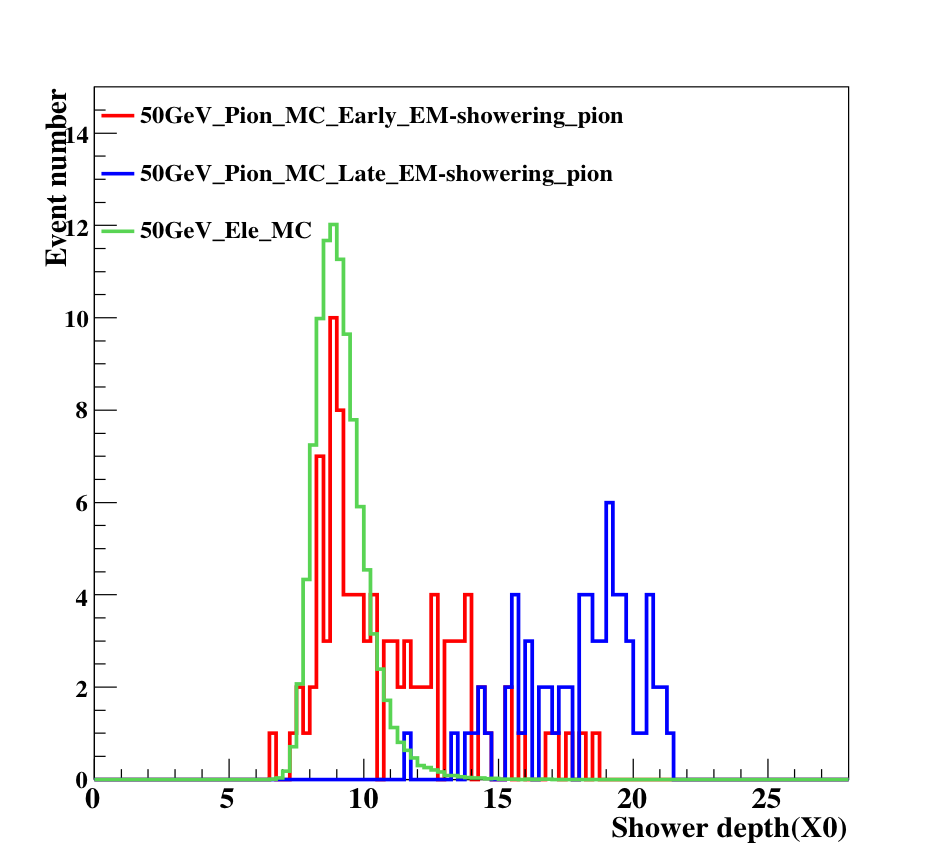
\includegraphics[width=\cmsFigWidth]{Delta-ray/Shower_depth_50GeV.png}
\caption{This figure shows the shower depth for both Early EM-showering and Late EM-showering.}
\label{HGCAL_shower_depth}
\end{figure}

\begin{figure}[!htb]
\centering
     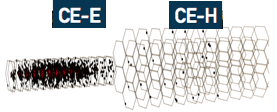
\includegraphics[width=0.45\textwidth]{Delta-ray/Normal_electron.png}
     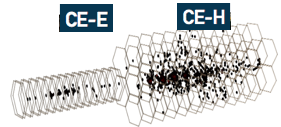
\includegraphics[width=0.45\textwidth]{Delta-ray/Normal_pion.png}\\
     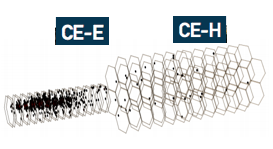
\includegraphics[width=0.45\textwidth]{Delta-ray/Early_EM-showering.png}
     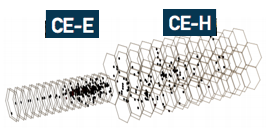
\includegraphics[width=0.45\textwidth]{Delta-ray/Late_EM-showering.png}
\caption{These figures show the event display with the cases which are the used to probe in the studies. (Top left) is the normal electron, most of the energy put in the CE-E, oppositely, (Top right) is the normal pion, which put most of the energy in CE-H. The both cases below the normal particles are the "e-like pion" cases, which we target to distinguish them from the normal electron. The left plot is the case for "Early EM-showering" and the right plot is the case for "Late  EM-showering".}
\label{Event_display}
\end{figure}

We show some event display for normal electron and pion showering, Early EM-showering and Late EM-showering in Fig.\ref{Event_display}. And we present the event display in the We used the cut that, we require a consecutive number of hits in CE-E starting from the first layer and checking until the 14 Layer. We record the first layer found with more than 3MIPs. And at least 2 consecutive layers with more than two seeds with Energy$>$3MIPs. If the layer of start showering is from the first to fifth layer, we called it "Early EM-showering", on the other hand, if it starts at sixth to later layers, we called it "Late EM-showering". For note, because this is the convenient way to let us see the dynamic of the shower in ECAL approximately, we used this cut to distinguish them. In the real case, we don't do this cut, just used one variable to distinguish "both" of them from electrons. I will show the results later. 

\begin{table}[h]%??table???????????????????[h]???????here?????????????
    \centering
    \begin{tabular}{|c|c|c|}
    \hline
    Tight cut types & value\\\hline
    5-Rings cut &  $>$ 0.99 \\\hline  
    The last layer energy & $<$ 20MIPs \\\hline  
   $\mathrm{\frac{E_{7}}{E_{19}}}$& $>$ 0.75\\\hline  
        \end{tabular}
    \caption{E10/Etotal Tight cuts selection used in June test-beam}\label{basic_1}  %????????????
\end{table}


Until now, we can see the one strong point of the difference between electron and e-like pion - the shower energy deposit in the ECAL. Because some of them put energy in the different section of succeeding layers in ECAL, specially for comparing the electrons with Late EM-showering. In this case, we thought about the variables with "longitudinal segmentation" with ECAL. We developed the discrimination variable as following:
\begin{equation}
\mathrm{E_{10}=\frac{E_{\mathrm{first \ 10 \ layers \ energy}}}{E_{\mathrm{total \ energy}}}}
\end{equation}

Intuitively, because the electrons put most of the energy in the front of the detector, they will have the bigger value for $\mathrm{E_{10}}}$. Oppositely, for the e-like pions, because they put all of the energy in the different sections, they will have many values for $\mathrm{E_{10}}}$ from all events. In the Fig.\ref{HGCAL_E10}, we can see that we can use $\mathrm{E_{10}}}$ to reject some of e-like pions out of the electron region. 

\begin{figure}[!htb]
\centering 
     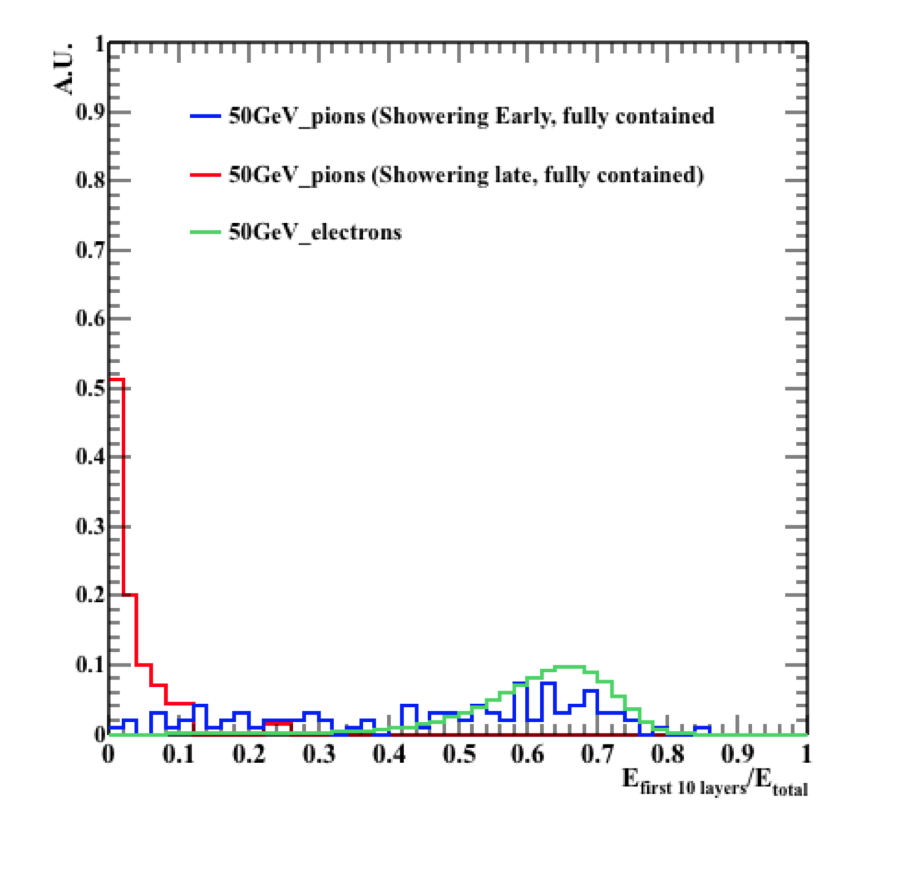
\includegraphics[width=\cmsFigWidth]{Delta-ray/E10_50GeV.png}
\caption{The E10 value for electrons, Early EM-showering and Late EM-showering.}
\label{HGCAL_E10}
\end{figure}

In my study, we need to find the critical point of $\mathrm{E_{10}}}$ to be the threshold, because we wanted to reserve the electrons as many as possible, and cut-off the bad pions for our best. 
We used the quantities about the "Electron Efficiency" and "Background Rejection" as our standard in the following formula, to see whether this cut is good:
\begin{equation}\label{Equation_SIG}
\mathrm{Electron \ Efficiency \ = \frac{Pass \ electrons}{Total \ electrons}}
\end{equation}
\begin{equation}\label{Equation_BKG}
\mathrm{Background \ Rejection \ = \frac{Total \ e\mathrm{-}like \ pions}{Pass \ e\mathrm{-}like \ pions}}
\end{equation}
Our goal is to cut-off the most e-like pion with the highest background rejection ( pass the least e-like pions ) in (\ref{Equation_SIG}), but reserve the most electrons with the highest electron efficiency. ( pass the most electrons ) in (\ref{Equation_BKG}).

First, we tried to use the critical point at 0.2, 0.3 and 0.4, and see whether it can give us the best results. In the Table.\ref{basic_10}}, it tells us that the background rejection is good ( more than half of e-like pions are rejected ), but we hoped that our electron efficiency will go to 99.8\% or more. On the other hand, we still wanted to keep the electrons alive after the higher critical point to reserve most important researches on them.

\begin{table}[h]%??table???????????????????[h]???????here?????????????
    \centering
    \begin{tabular}{|l|c|c|}
    \hline
    E10/Etotal cut  & Background Rejection  &  Electrons Efficiency\\\hline
    $>$0.2 & 2.15+/-0.18(stat)   & 99.85\%+/-0.01\%(stat) \\\hline
    $>$0.3 & 2.53+/-0.24(stat)   & 99.30\%+/-0.01\%(stat) \\\hline
    $>$0.4 & 2.74+/-0.28(stat)   & 97.32\%+/-0.01\%(stat) \\\hline
    \end{tabular}
    \caption{E10 cuts of Electrons Efficiency and Background Rejection comparison with point 0.2,0.3 and 0.4}\label{basic_10}  %????????????
\end{table}

In this case, we tried to use another points near 0.2 and see whether we can get the great results without losing more electrons. In the Table.\ref{basic_20}, it said that near the point 0.2, it can reserve most of the electrons near 99.9\% and can get the background rejection with the expectation value near 2 (Half of rejection). 

\begin{table}[h]%??table???????????????????[h]???????here?????????????
    \centering
    \begin{tabular}{|l|c|c|}
    \hline
    E10/Etotal cut  & Background Rejection  &  Electrons Efficiency\\\hline
    $>$0.16 & 2.02+/-0.15(stat)   & 99.93\%+/-0.01\%(stat) \\\hline
    $>$0.18 & 2.07+/-0.16(stat)   & 99.89\%+/-0.01\%(stat) \\\hline
    $>$0.20 & 2.15+/-0.17(stat)   & 99.85\%+/-0.01\%(stat) \\\hline
    \end{tabular}
    \caption{E10 cuts of Electrons Efficiency and Background Rejection comparison with point 0.16,0.18 and 0.20}\label{basic_20}  %????????????
\end{table}

For the conclusion of this month test-beam results, we found that the Background Rejection can be near 2 without killing many electrons with 99.9\% Electron Efficiency. For our expectation, we wanted to apply this cut in the October test-beam, to see whether we can see the similar results. 

\subsection{The results of application in October test-beam MC}
In this month test-beam, because we had the information of HCAL, we used the cut no more than 0.4\% energy fraction in the HCAL energy to replace the poor man's solution. And also, we changed some parameters of the cuts to get the best results. In the Table.\ref{basic_100}, the summary table for the cuts is shown.

\begin{table}[h]%??table???????????????????[h]???????here?????????????
    \centering
    \begin{tabular}{|c|c|c|}
    \hline
    Tight cut types & value\\\hline
    5-Rings cut &  $>$ 0.99 \\\hline  
    $\frac{\mathrm{HCAL  \ total \  energy}}{\mathrm{ECAL \ total \ energy}}$ & $<$ 0.004 \\\hline  
    $\mathrm{\frac{E_{7}}{E_{19}}}$ & $>$ 0.85\\\hline  
        \end{tabular}
    \caption{Tight cuts selection used in October test-beam}\label{basic_100}  %????????????
\end{table}

In the June test-beam, we only did the rejection for $\mathrm{E_{10}}$ after the tight-cut selections. In this month, we wanted to studied the power of the cuts from tight-cut selections to $\mathrm{E_{10}}$, it means we wanted to study totally how many e-like pions will be rejected after all cuts.  We have two steps rejection, and we used the same definitions with the equation (\ref{Equation_SIG}) and (\ref{Equation_BKG}).
\begin{itemize}
\item Tight cuts rejection power: \\ 
This is the first step rejection study. Because we need to find out the e-like pions with the cut in the Table.\ref{basic_100} first, and then we can use our segmentation variable to reject them for the next step.  For this step, we found that the number of the background rejection is 3600. Most of the pions are rejected by those cuts.
\item $\mathrm{E_{10}}$ cuts rejection power:\\
This is the second step rejection study. After we found out the e-like pions, we used the discrimination variable which we have invited in June test-beam,$\mathrm{E_{10}}$, to distinguish them from the real electrons. In this step, we used the critical point at 0.18,0.20 and 0.22, to see whether at the critical point near 0.2 will give us the good results. In the Table.\ref{basic_7} summarize the results for them. 
Although, this time didn't have the better results compared with the June test-beam, we still got the number about 1.5.
\end{itemize}
\begin{table}[h]%??table???????????????????[h]???????here?????????????
    \centering
    \begin{tabular}{|l|c|c|}
    \hline
    E10/Etotal cut & Electron Efficiency & Background Rejection\\\hline
    $>$ 0.18 &  99.56\%+/-0.01\%(syst)+/-0.20\%(stat) &  1.52+/-0.27(stat)\\\hline  
    $>$ 0.20 &  99.05\%+/-0.01\%(syst)+/-0.20\%(stat) &  1.53+/-0.26(stat)\\\hline  
    $>$ 0.22 &  98.91\%+/-0.01\%(syst)+/-0.20\%(stat) &  1.56+/-0.24(stat)\\\hline  
        \end{tabular}
    \caption{E10 cuts electrons efficiency and Background rejection after the tight cuts}\label{basic_7}  %????????????
\end{table}


In the end, totally we can get the total rejection power of cuts which is calculated by the number 3600 with the Tight cuts rejection power and the number 1.5 with the $\mathrm{E_{10}}$ cuts rejection power. After times them together, we can get the number $3600\times1.5=5400$. In A Toroidal LHC ApparatuS(ATLAS), the expected value for it is between 5000 to 10000, and in our case, we arrived the value for the expectation. 
\subsection{Conclusion}
In this section, we obtained the cuts and new variable $\mathrm{E_{10}}$ to distinguish the e-like pions from real electrons with the June test-beam MC samples, and we applied in the October test-beam MC samples, happily, we got the expected results compared with the previous studies in ATLAS. This cuts and variable have never been applied in CMS analysis before, and we expect that we can help to reduce the background which is sensitive to electron/pion identification with HGCAL in the future.

\section{Studies of granularity of a hadronic calorimeter for tens-of-TeV jets at a 100 TeV $pp$ collider}
After the discovery of the standard-model-like Higgs boson at 2012\cite{Chatrchyan:2012xdj}, we have established a milestone in HEP field. We used the LHC at CERN to solve an important puzzle in the SM of particle physics, Higgs boson, and it gave us the answer why the elementary particles retain their mass\cite{PhysRevLett.13.508} from the early universe to now. We expect more particles predicted by BSM can be found in the future. A lot of these new particles may be heavier than 13 TeV\cite{Contino:2016spe}\cite{Mangano:2016jyj}, which is operating now in LHC. Therefore, particle physicists plan to build a very high energy collider with $\sqrt{s} = 100\TeV$ in the future, such as high-energy LHC (HE-LHC), future circular $pp$ colliders of the European initiative, FCC-hh~\cite{Benedikt:2206376} and the Chinese initiative, SppC~\cite{Tang:2015qga}. \\

In the very high energy era, the C.M. energy will be increased compared with now in LHC, and the instantaneous luminosity is also expected to increase. In this case, more interesting events will occur within a shorter amount of time, but incidentally, it will accompany with the unexpected background. We need to figure out some methods to pick out the signals which we are interested in, and filter the unwanted huge background events extremely. The silicon future circular collider (SiFCC) detector, which is based on the silicon detector (SiD)\cite{Aihara:2009ad} designed for international linear collider (ILC)\cite{Adolphsen:2013kya}\cite{Behnke:2013lya}, is our simulated detector prepared for the high energy collider for the future era in Ref.\cite{Chekanov:2016ppq}.We used this detector to simulate the condition under very high C.M., and applied the different configurations of detector with some methods such as jet substructure variables, to see the detector performance of distinguishing the signal from background. I will describe the detail later.\\

Traditionally, we used scintillators as the active layers of the ECAL and HCAL to measure the energy of the showering of particles which are induced by the absorbers (with material such as lead, brass, or tungsten, etc.). But when the radiation dosage is much higher than before, scintillators can deteriorate easily. This is the same circumstance which CMS is bumped into now. In addition, because of time consuming for making the special shape for fitting the detector, it is not easy to sub-divide scintillators into smaller areas. And also, we need to have a readout with high position resolution to match them. In this case, we want to use the new design- "high granularity" detector to resolve the resolution problems, i.e., we used the different configurations of detector to record the precise position and energies. For the radiation problem, because the silicon detector is known to be radiation tolerant.\cite{Li:2002ru}, we could use it in the future collider, same as HGCAL which was presented in my previous studies.\\

I did this study with Prof. Shin-Shan Eiko Yu from NCU, Prof. Ashutosh Kotwal and student Sourvan Sen from Duke University, Dr. Sergei Chekanov and Dr. Proudfoot James from Argonne National Laboratory(ANL), and Nhan Viet Tran from Fermi National Accelerator Laboratory. The contributions of Chih-Hsiang Yeh to this study includes the following:
\begin{itemize}
\item Study of detector performance with soft drop mass.
\item Studies of signal and background separation using the different jet substructure variables.
\end{itemize}
I will describe the detail as following.

\subsection{Simulation of detector response and event reconstruction}
 
The description of the detector and software used for our study is discussed in \cite{Chekanov:2016ppq}. We used the geometry of SiFCC detector with the software package that represents a various environment for simulations of detector performance. It is used to prepare for new technology options, event reconstruction techniques for future 100~TeV colliders. Figure \ref{fig:SiFCC} is the SiFCC detector simulated by the {\sc geant4} package\cite{Allison2016186} and it was the detector studied in Ref.\cite{Chekanov:2016ppq}. The baseline detector discussed in \cite{Chekanov:2016ppq} uses a steel-scintillator hadronic calorimeter with a transverse cell size of 5~$\times$~5~cm$^2$, which corresponds to $\Delta \eta \times \Delta \phi = 0.022\times0.022$. In addition, because we wanted to test the detector performance of granularity effect with hadronic processes of signal and background, several geometry variations were considered, such as 20~$\times$~20~cm$^2$ and  1~$\times$~1~cm$^2$, which correspond to $\Delta \eta \times \Delta \phi$= $0.087\times0.087$ and  $0.0043\times0.0043$, respectively.\\

\begin{figure}
\begin{center}
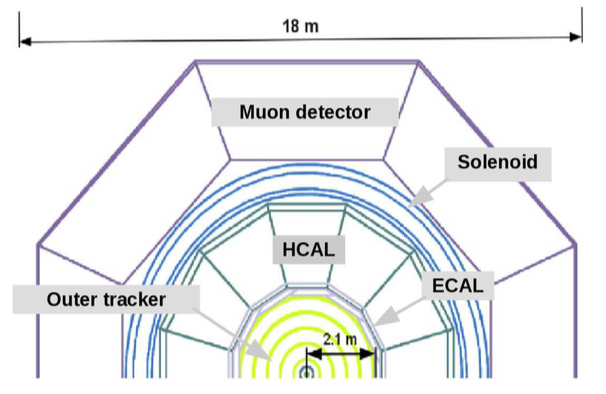
\includegraphics[width=0.6\textwidth]{figs/6.png}
\end{center}
\caption{The azimuthal cross section of the SiFCC detector.}
\label{fig:SiFCC}
\end{figure}

SiFCC detector which was simulated in our study contains five main parts: tracker, ECAL, HCAL, solenoid, and muon chambers. When particles are produced in the collider, they will go through the detector and leave signals to be recorded. First, the tracker can record the trajectory of a charged particle because it can leave the energy in and bended by the solenoid, we can obtain the transverse momentum of this charged particle. Electrons and photons will leave energy in ECAL , and hadronic particles, such as neutrons, protons, etc., will deposit energy in HCAL mainly. Muons will go through the whole detector and could be detected by muon chamber. Figure \ref{fig:barrel_size_material} lists the material and the configuration for the sub-detectors in SiFCC. Note, since for the time being we have more experimental results coming from the scintillator-based HCAL in CMS and ATLAS, we have been using this type of HCAL as a first study. After finishing the first study, we will move to the study of HCAL with silicon sensors as active layers later, same as HGCAL material. 


In our studies, we used the simulations of a heavy $Z'$ boson, a hypothetical gauge boson that arises from extensions of the electroweak symmetry of the SM.
The $Z'$ bosons were simulated with the masses, $M=5$, $10$, $20$ and $40$~TeV. The lowest value $5$~TeV represents a mass that is the achieved C.M energy of the LHC experiments. The value $40$~TeV represents the physics for 100~TeV colliders. The $Z'$ particles are forced to decay to two light-flavor jets ($\mathrm{q\bar{q}}$) with one-prong jet as background, $\mathrm{W^+W^-}$ or $\mathrm{t\bar{t}}$ as signal, where $\mathrm{W(\rightarrow q\bar{q})}$ with two-prong jets, and $\mathrm{t (\rightarrow  W^+\>b \rightarrow q\bar{q} b)}$ with three-prong jets decay hadronically. The processes for signal and background are shown in Fig.\ref{fig:Process_SB}. In all such scenarios, two highly boosted jets are produced, which are typically back-to-back in the laboratory frame. The main difference between considered decay types lays in different jet substructure. The events of signals were generated using the \pythia generator with the default settings, ignoring interference with SM processes. The event samples which were used in this paper are available from the HepSim database~\cite{Chekanov:2014fga}.

\begin{figure}
\begin{center}
   \subfigure[Background Z'$\rightarrow$ q$\bar{\mathrm{q}}$] {
   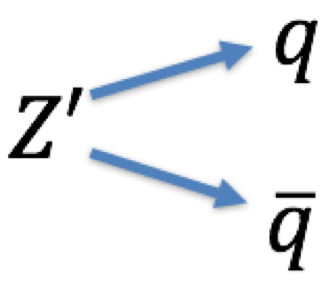
\includegraphics[width=0.25\textwidth]{figs/10.png}\hfill
   }
   \subfigure[Signal Z'$\rightarrow$WW] {
   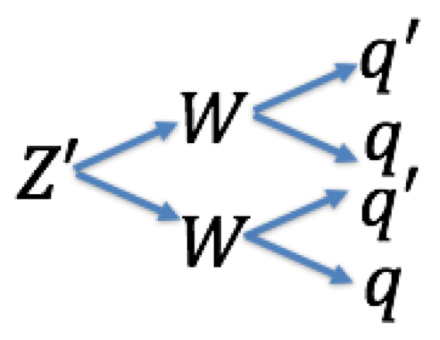
\includegraphics[width=0.25\textwidth]{figs/11.png}
   }
    \subfigure[Signal Z'$\rightarrow$ t$\bar{\mathrm{t}}$] {
   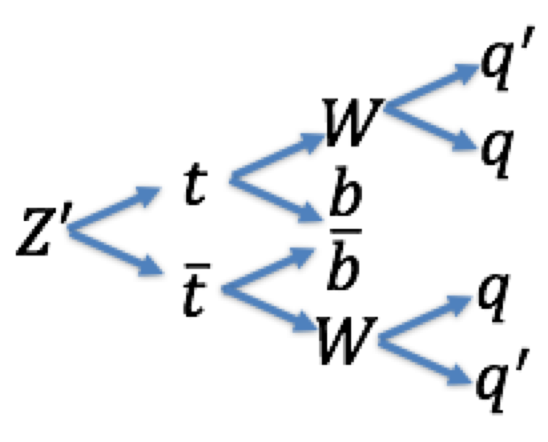
\includegraphics[width=0.25\textwidth]{figs/12.png}
   }

\end{center}
\caption{The signals and background we study.}
\label{fig:Process_SB}
\end{figure}

%%%===============================Soft_drop_mass================================%%
\subsection{Study of detector performance with soft drop mass}
In this section, we use the jet mass computed with a specific algorithm, soft 
drop declustering, to study the performance of detector with various detector 
cell sizes and center-of-mass (c.m.) energies. 
\subsubsection{The technique of soft drop declustering}
The soft drop declustering~\cite{Larkoski:2014wba} is a grooming method 
that removes soft wide-angle radiation from a jet. The constituents of a jet 
$j_0$ are first reclustered using the Cambridge-Aachen
 (C/A) algorithm~\cite{Dokshitzer:1997in,Wobisch:1998wt}. Then, the jet $j_0$ 
is broken into two subjets $j_1$ and $j_2$ by undoing the last stage of C/A 
clustering.
If the subjets pass the following soft drop condition, jet $j_0$ is the final 
soft-drop jet. Otherwise, the algorithm redefines $j_0$ to be the subjet with 
larger $p_T$ (among $j_1$ and $j_2$) and iterates the procedure.
\begin{equation} \label{eq:soft-drop}
\frac{\mathrm{min}(p_{T1},p_{T2})}{p_{T1}+p_{T2}}>z_\mathrm{cut}(\frac{\Delta R_{12}}{R_{0}})^{\beta},
\end{equation}
where $p_{T1}$ and $p_{T2}$ are the transverse momenta of the two subjets, 
$z_\mathrm{cut}$ is soft drop threshold, 
$\Delta R_{12}$ is the distance between the two subjets in the $\eta$-$\phi$ 
plane, $R_0$ is the characteristic radius of the original jet, and $\beta$ is 
the angular exponent.

In our study, we compare the performance of future detector when setting 
$\beta=0$ versus when setting $\beta=2$. For $\beta=0$, the soft drop condition 
depends only on the $z_\mathrm{cut}$. For $\beta=2$, the condition depends on 
the angular distance between the two subjets and $z_\mathrm{cut}$ and the 
algorithm becomes infrared and collinear safe. 

\subsubsection{Analysis method}\label{Analysis_method}
We employ the following method to quantify the detector performance and 
find out the cell size that gives the best separation power to distinguish 
signal from background. For each configuration of detector and c.m. energy, 
we draw the receiver operating characteristic (ROC) curves in which the x-axis
 is the signal efficiency ($\epsilon_\mathrm{sig}$) and y-axis is the inverse 
of background efficiency ($1/\epsilon_\mathrm{bkg}$). 
In order to scan the efficiencies of soft drop mass cuts, we vary the mass 
window as follows. We first look for the median bin 
$i_\mathrm{med}$\footnote{The integral from bin 0 to bin $i_\mathrm{med}$ 
($i_\mathrm{med}-1$) should be greater (less) than half 
of the total number of events. Note, the bin width is 5~GeV.} of the soft 
drop mass histogram from simulated signal events. Taking the right boundary
 of bin $i_\mathrm{med}$ as the center of mass window 
$x_\mathrm{center}$, we start increasing the width of mass window symmetrically
 on the left and on the right of $x_\mathrm{center}$, in steps of 5~GeV, 
i.e. the narrowest mass window is 
[$x_\mathrm{center}-5,x_\mathrm{center}+5$]. If one side reaches the boundary 
of the mass histogram, we only increase the width on the other side, also in 
steps of 5~GeV. For each mass window, there will be corresponding 
$\epsilon_\mathrm{sig}$ and $\epsilon_\mathrm{bkg}$, which gives a point in 
the ROC curves.

\subsubsection{Results and conclusion}
Figures~\ref{fig:cluster_mass_mmdt_ww}, \ref{fig:cluster_mass_mmdt_tt},
 \ref{fig:cluster_mass_sdb2_ww}, and \ref{fig:cluster_mass_sdb2_tt} 
present the distributions of soft drop mass for $\beta=0$ and $\beta=2$ with 
different c.m. energies and detector cell sizes; the signals considered are 
Z'$\rightarrow$WW and Z'$\rightarrow$t$\bar{\mathrm{t}}$. 
In Figs.~\ref{fig:cluster_mass_mmdt_ww_ROC}, \ref{fig:cluster_mass_mmdt_tt_ROC}, \ref{fig:cluster_mass_sdb2_ww_ROC}, and \ref{fig:cluster_mass_sdb2_tt_ROC}, 
ROC curves from different detector cell sizes are compared for each 
c.m. energy, respectively. 

Figures~\ref{fig:cluster_mass_mmdt_ww_ROC} and 
\ref{fig:cluster_mass_mmdt_tt_ROC} show that for $\beta=0$ the 
smallest detector cell size, 
 $1~\mathrm{cm}\times1~\mathrm{cm}$, has the best separation power at 
$\sqrt{s}=$5, 10, and 20~TeV when the signal is Z'$\rightarrow$WW and 
at  $\sqrt{s}=$10 and 20~TeV when the signal is Z'$\rightarrow$t$\bar{\mathrm{t}}$.
On the contrary, Figs.~\ref{fig:cluster_mass_sdb2_ww_ROC} and \ref{fig:cluster_mass_sdb2_tt_ROC} show that for $\beta=2$ the smallest detector cell size 
does not have improvements in the separation power with respect to those with 
larger cell sizes. In fact, the performances of the three cell sizes are 
similar. In addition, sometimes bigger detector cell sizes, 
$5~\mathrm{cm}\times5~\mathrm{cm}$ or $20~\mathrm{cm}\times20~\mathrm{cm}$
 have the best separation power. 

We also find compared to $\beta=2$, soft drop mass with $\beta=0$ has better 
performance for distinguishing signal from background. Therefore, we will 
apply requirements on this variable when studying the other jet substructure 
variables. 
 
%50bins
\begin{figure}
\begin{center}
   \subfigure[20~TeV at 20$\times$20 (cm$\times$cm) with cluster] {
   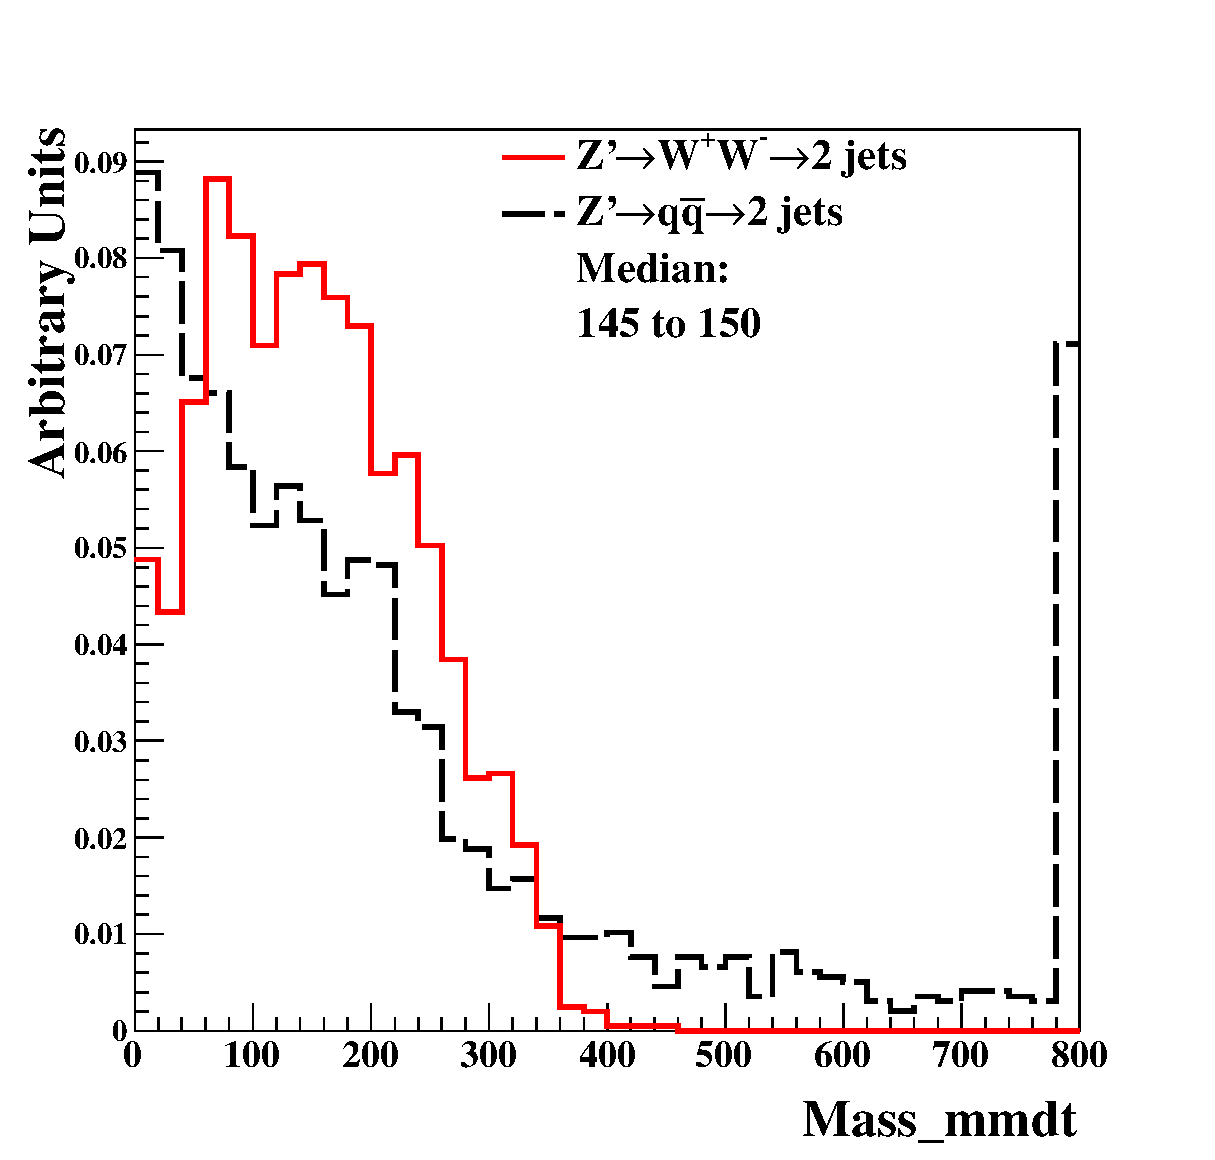
\includegraphics[width=0.25\textwidth]{figs/Dis_cluster_010_mass_mmdt_20tev_04_no_UOF.eps}
   }
      \subfigure[20~TeV at 5$\times$5 (cm$\times$cm) with cluster] {
   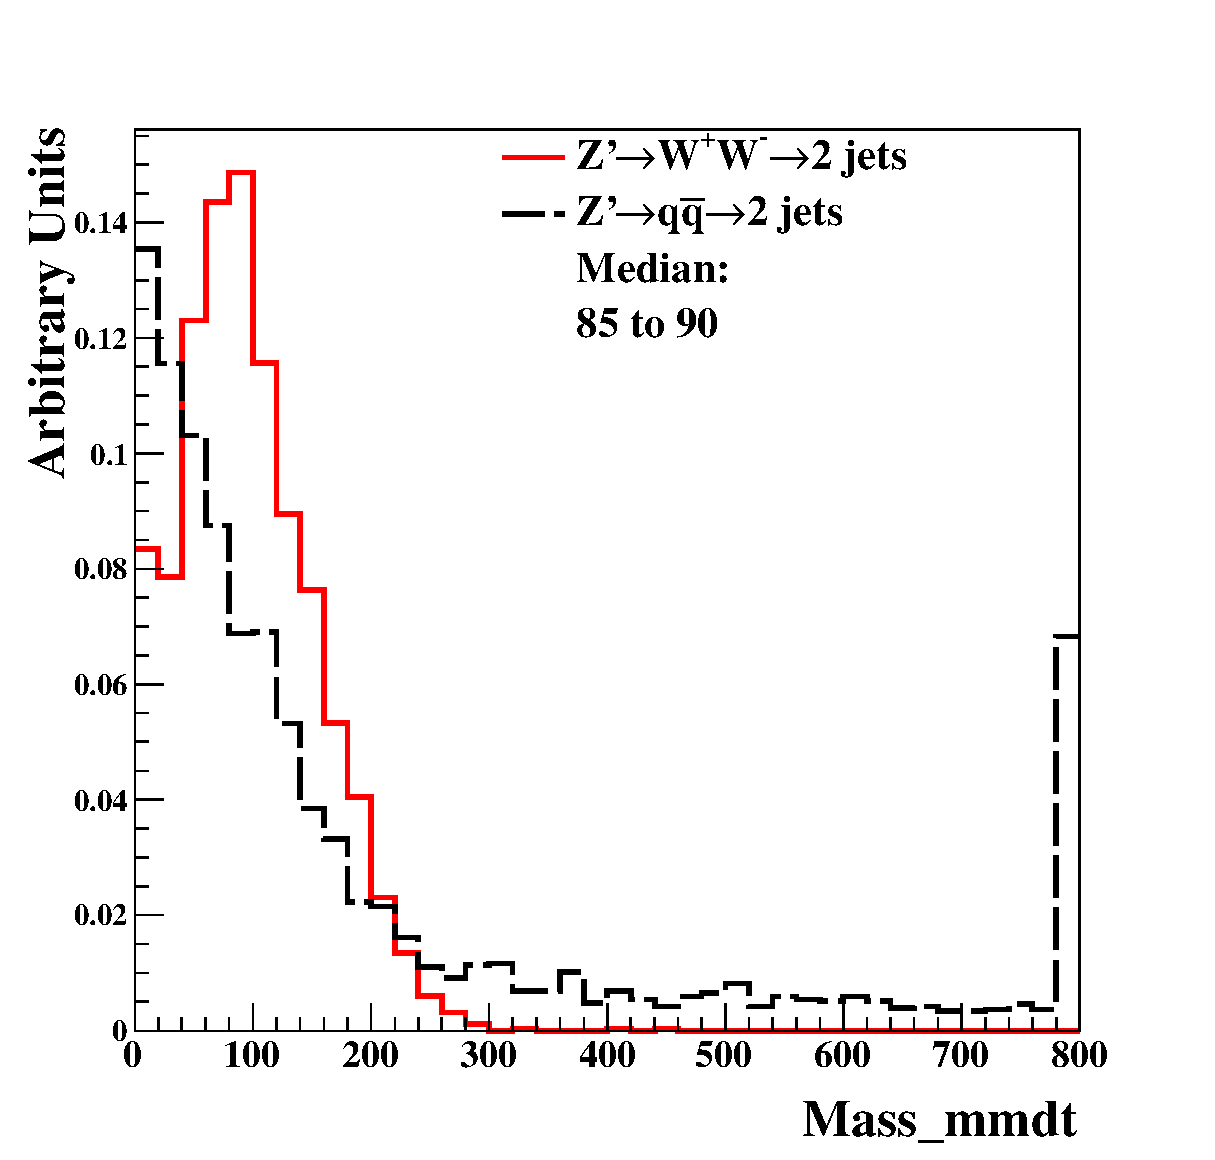
\includegraphics[width=0.25\textwidth]{figs/Dis_cluster_009_mass_mmdt_20tev_04_no_UOF.eps}\hfill
   }
   \subfigure[20~TeV at 1$\times$1 (cm$\times$cm) with cluster] {
   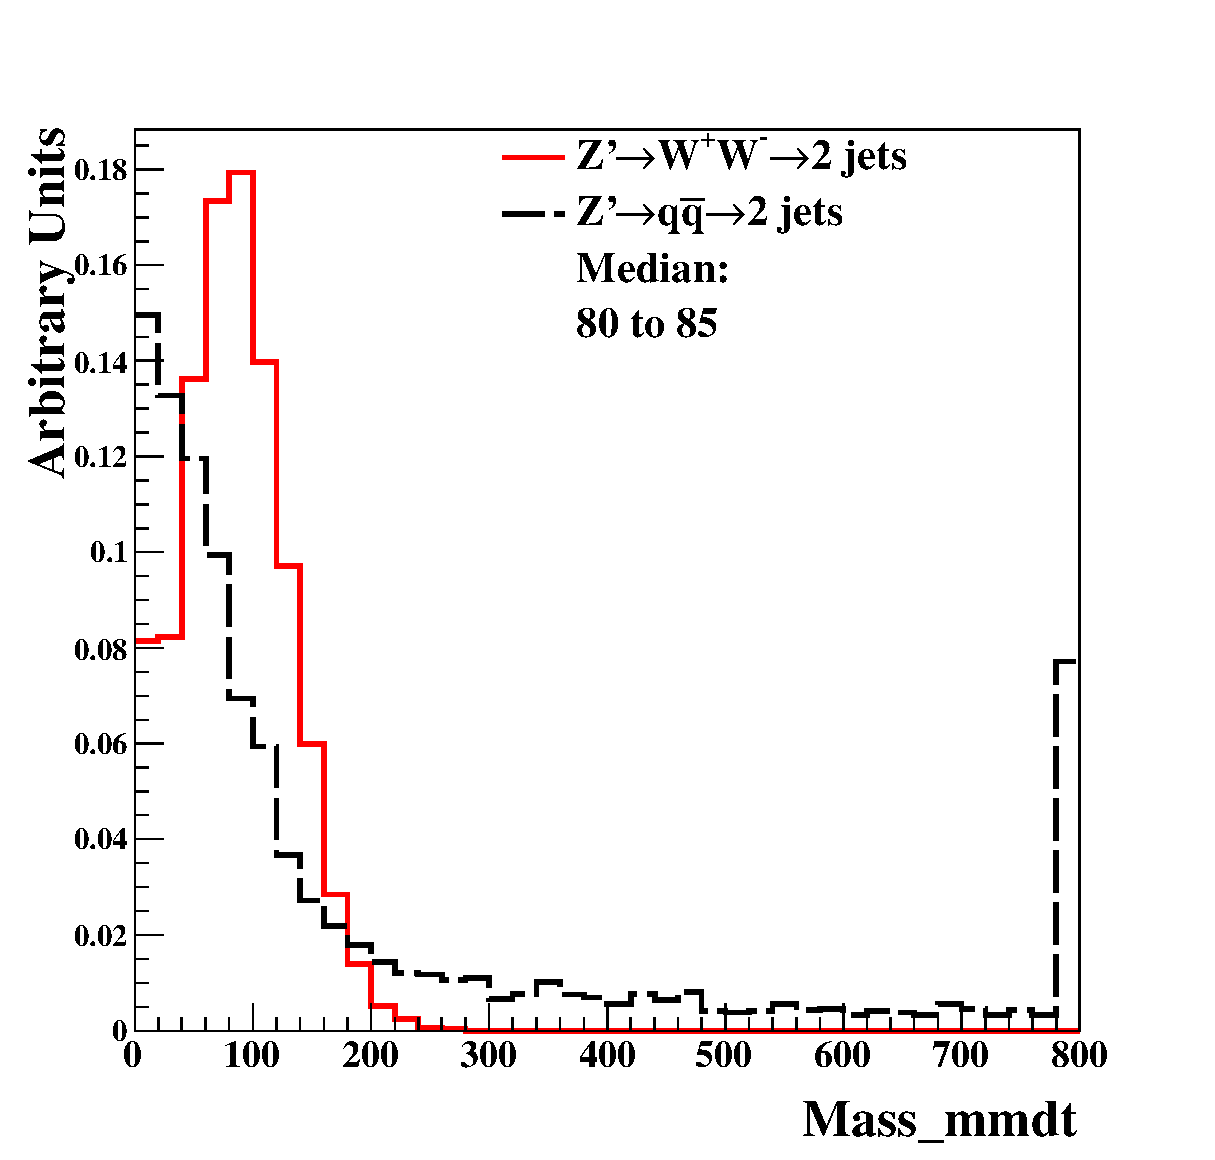
\includegraphics[width=0.25\textwidth]{figs/Dis_cluster_012_mass_mmdt_20tev_04_no_UOF.eps}\hfill
   }
\end{center}
\caption{Distributions of soft drop mass for $\beta$=0, with 5, 10, 20, and 
40~TeV c.m. energies and three different detector cell sizes: 20$\times$20, 
5$\times$5, and 1$\times$1 (cm$\times$cm). The signal (background) process is 
Z'$\rightarrow$WW (Z'$\rightarrow$q$\bar{\mathrm{q}}$).
\label{fig:cluster_mass_mmdt_ww}}
\end{figure}


\begin{figure}
\begin{center}
  \subfigure[$M(Z')=5$~TeV] {
  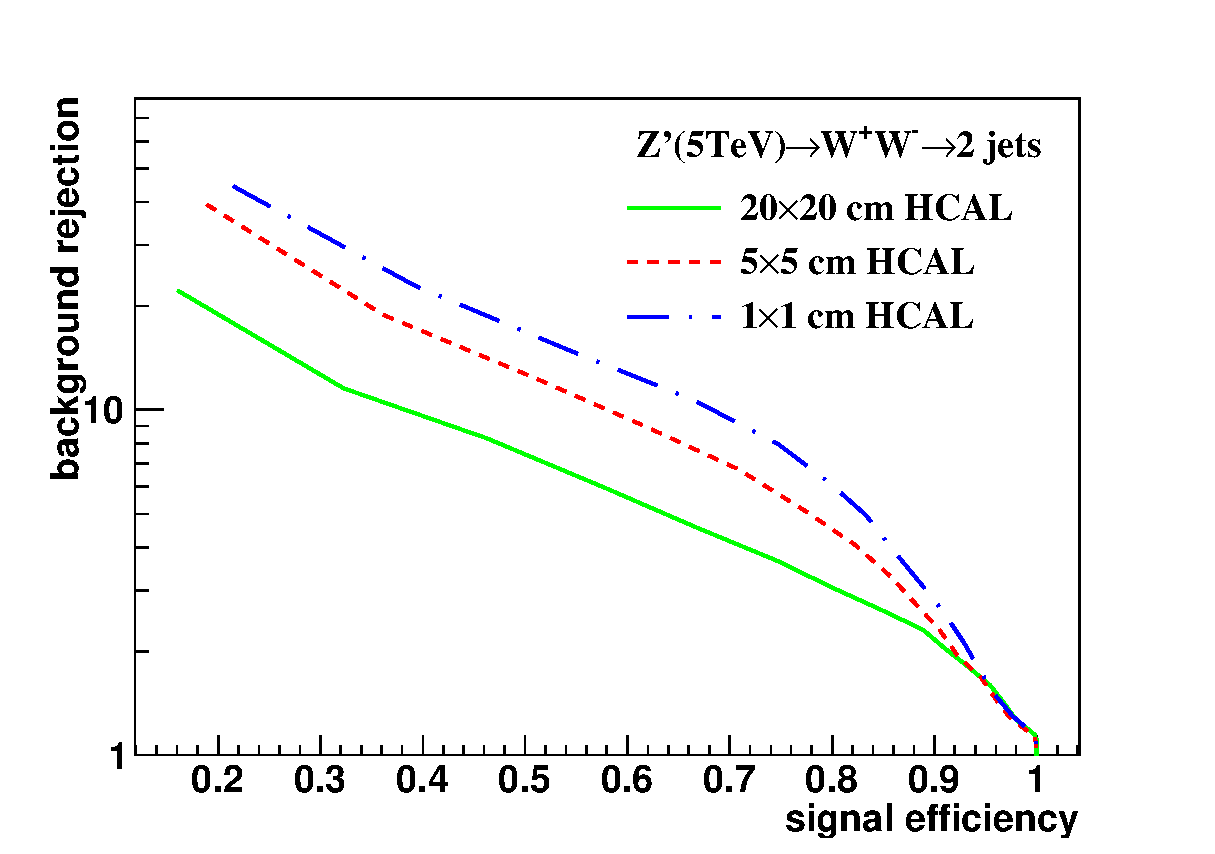
\includegraphics[width=\cmsFigWidth]{figs/A_Cluster_mass_mmdt_5tev_eff_1_central_fix_at_Median_bin_ww_qq_log_no_UOF.eps}
  }
  \subfigure[$M(Z')=10$~TeV] {
  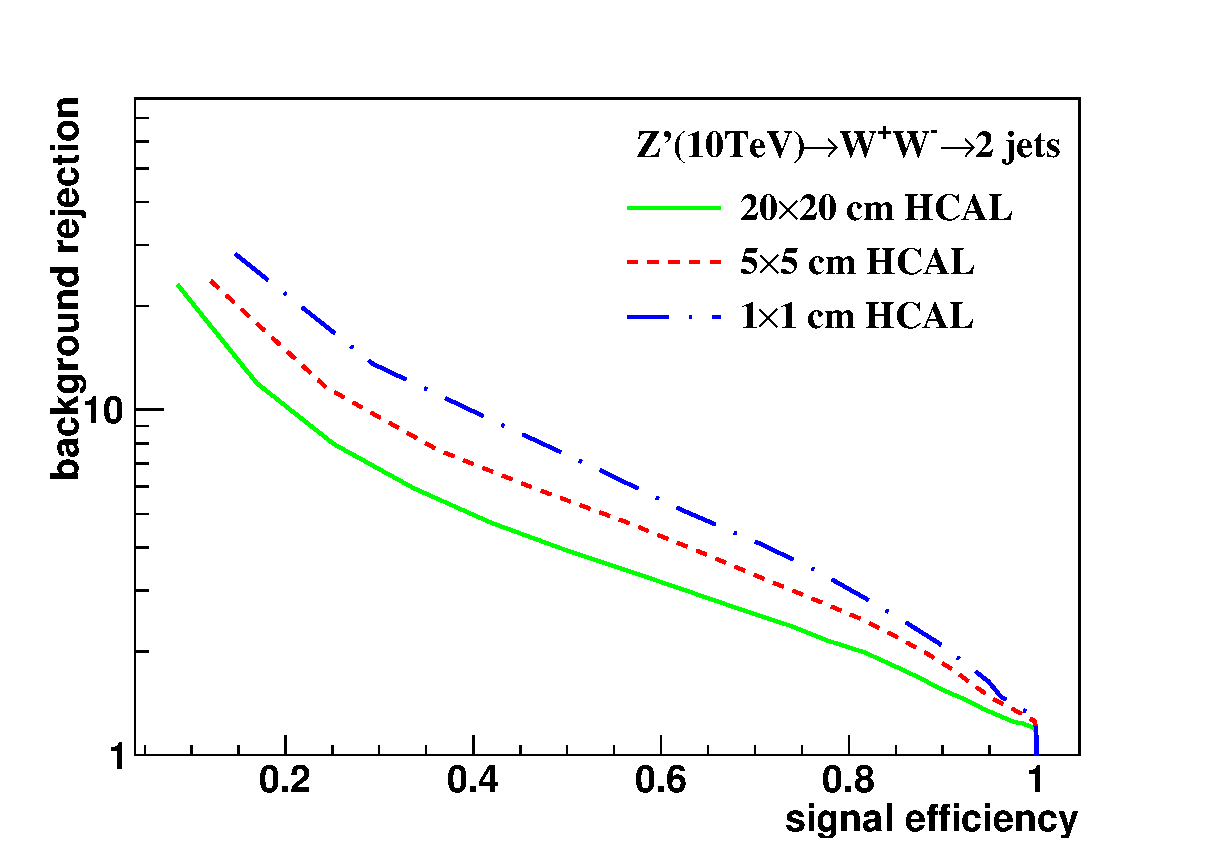
\includegraphics[width=\cmsFigWidth]{figs/A_Cluster_mass_mmdt_10tev_eff_1_central_fix_at_Median_bin_ww_qq_log_no_UOF.eps}
  }\\
 \subfigure[$M(Z')=20$~TeV] {
 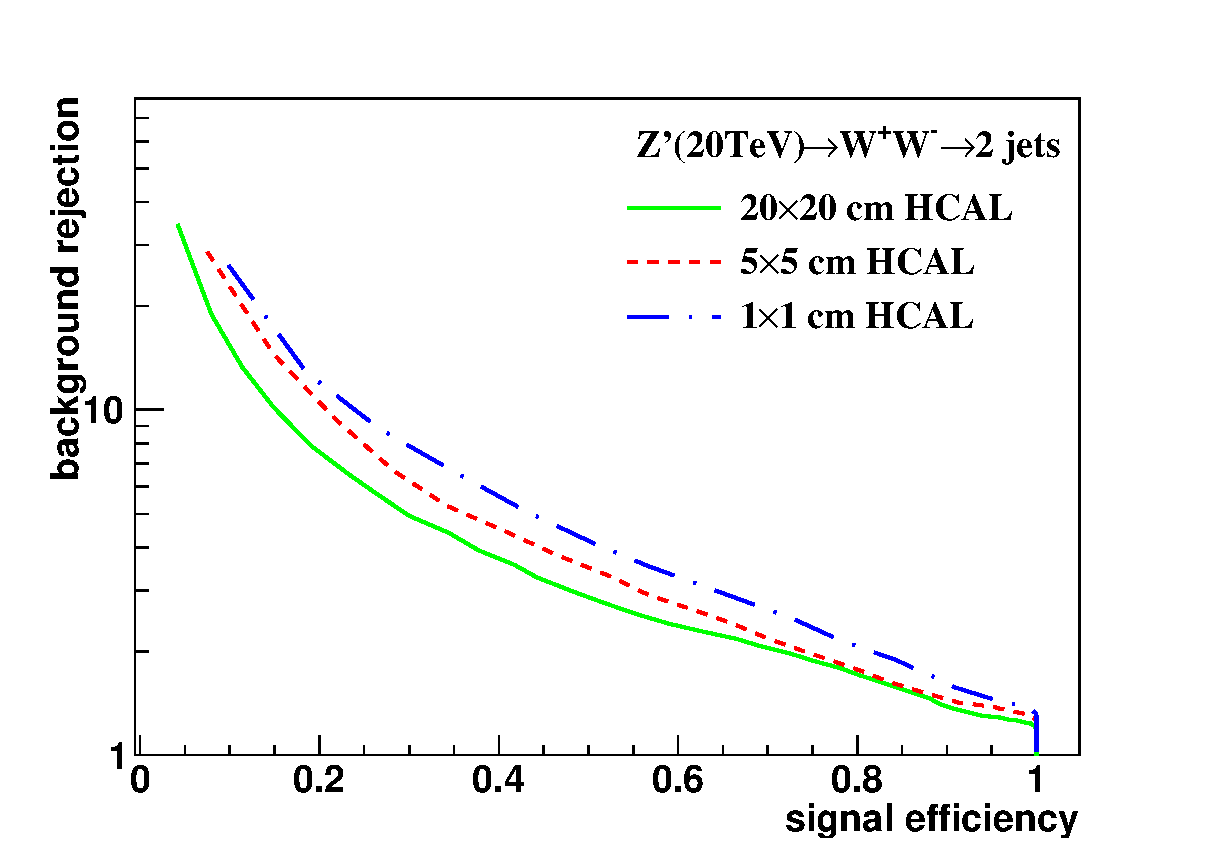
\includegraphics[width=\cmsFigWidth]{figs/A_Cluster_mass_mmdt_20tev_eff_1_central_fix_at_Median_bin_ww_qq_log_no_UOF.eps}
 }
 \subfigure[$M(Z')=40$~TeV] {
 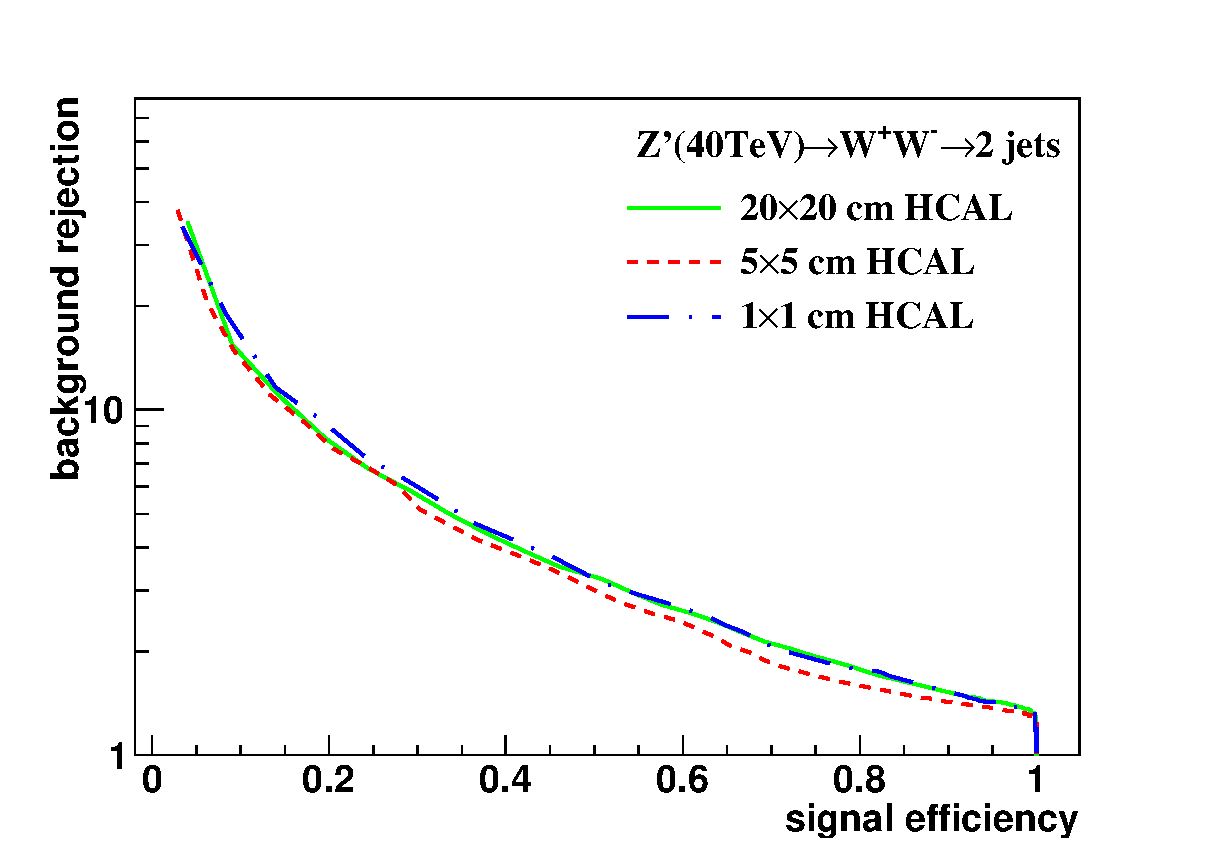
\includegraphics[width=\cmsFigWidth]{figs/A_Cluster_mass_mmdt_40tev_eff_1_central_fix_at_Median_bin_ww_qq_log_no_UOF.eps}
 }
\end{center}
\caption{The ROC curves of soft drop mass selection for $\beta$=0 
with 5, 10, 20, and 40~TeV c.m. energies. 
Three different detector cell sizes are compared: 20$\times$20, 
5$\times$5, and 1$\times$1 (cm$\times$cm). 
The signal (background) process is Z'$\rightarrow$WW 
(Z'$\rightarrow$q$\bar{\mathrm{q}}$).}
\label{fig:cluster_mass_mmdt_ww_ROC}
\end{figure}


\begin{figure}
\begin{center}
   \subfigure[20~TeV at 5$\times$5 (cm$\times$cm) with cluster] {
   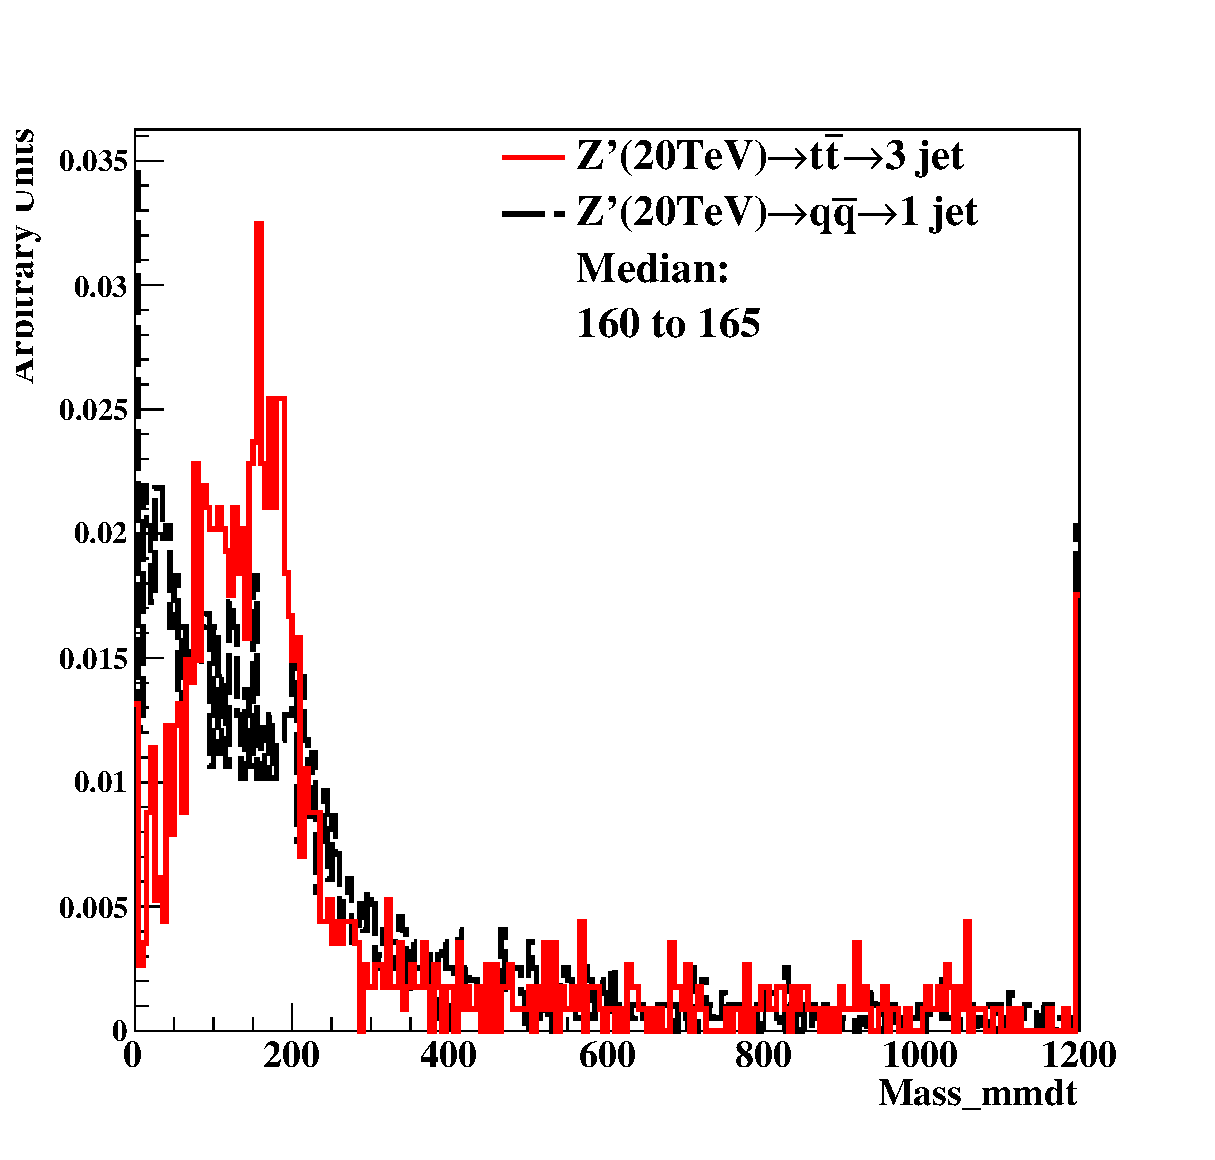
\includegraphics[width=0.25\textwidth]{figs/Dis_cluster_010_mass_mmdt_tt_20tev_04_tt_no_UOF.eps}
   }
   \subfigure[20~TeV at 20$\times$20 (cm$\times$cm) with cluster] {
   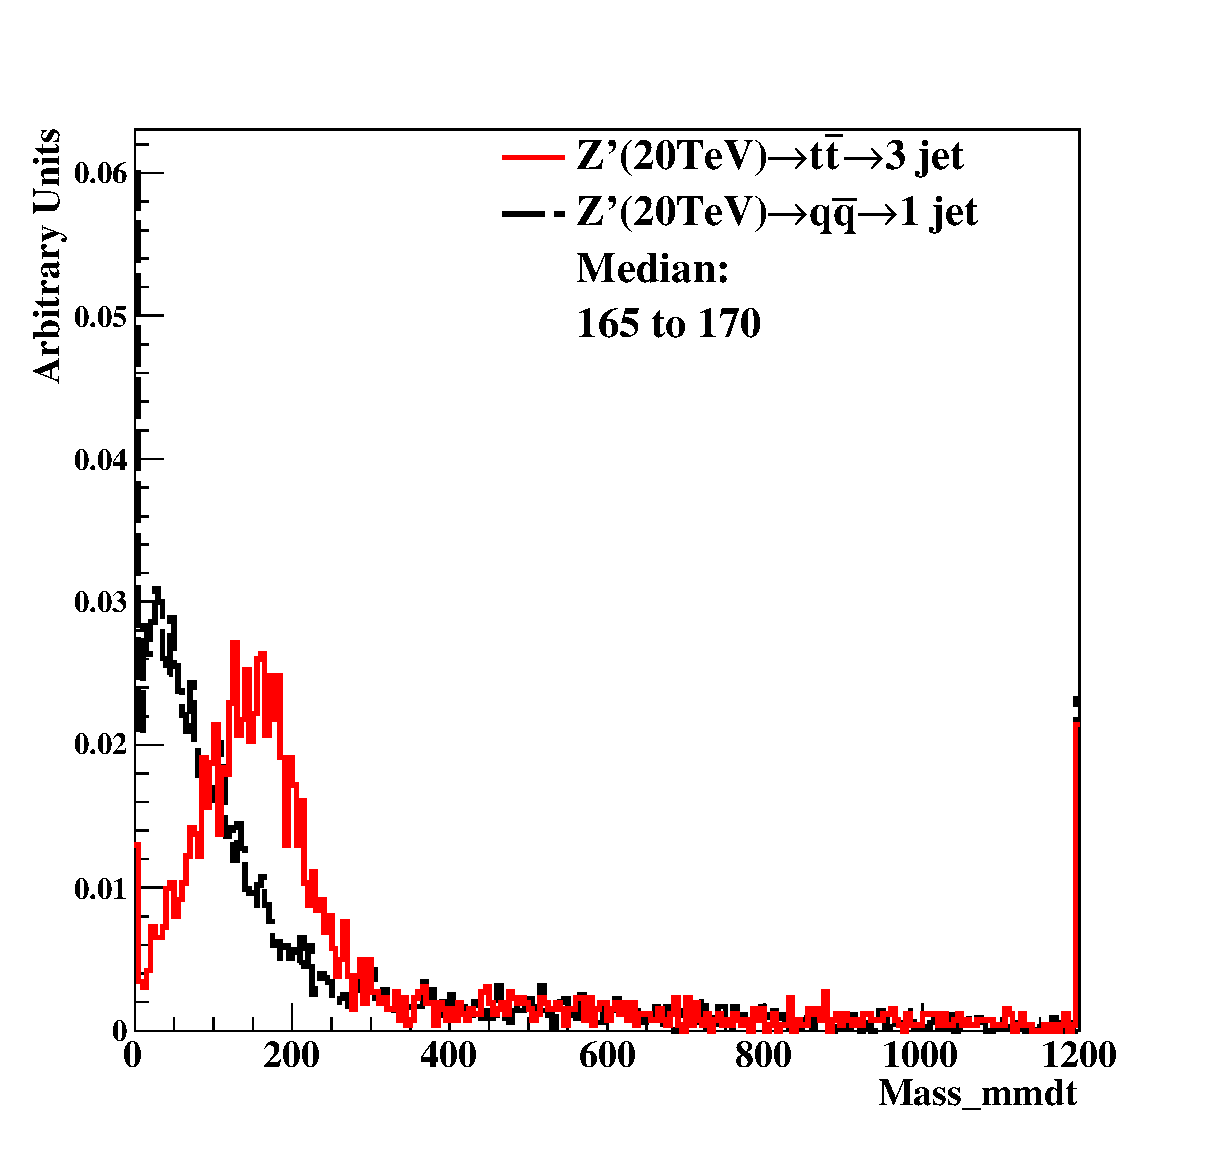
\includegraphics[width=0.25\textwidth]{figs/Dis_cluster_009_mass_mmdt_tt_20tev_04_tt_no_UOF.eps}\hfill
   }
   \subfigure[20~TeV at 1$\times$1 (cm$\times$cm) with cluster] {
   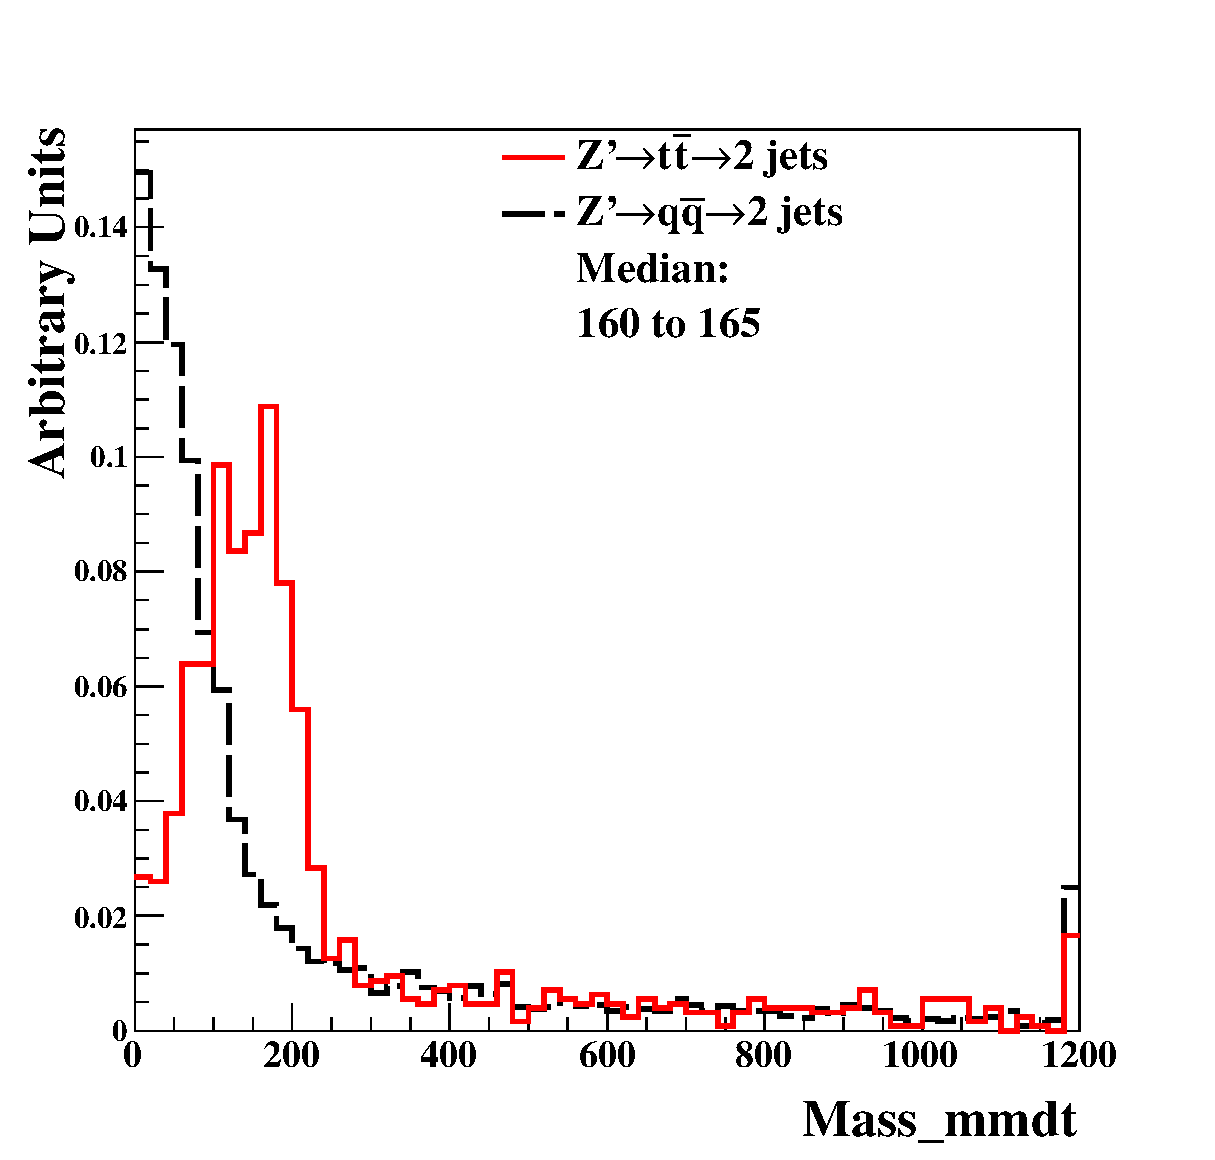
\includegraphics[width=0.25\textwidth]{figs/Dis_cluster_012_mass_mmdt_tt_20tev_04_tt_no_UOF.eps}\hfill
   }
\end{center}
\caption{
Distributions of soft drop mass for $\beta$=0, with 5, 10, 20, and 
40~TeV c.m. energies and three different detector cell sizes: 20$\times$20, 
5$\times$5, and 1$\times$1 (cm$\times$cm). The signal (background) process is 
Z'$\rightarrow$t$\bar{\mathrm{t}}$ (Z'$\rightarrow$q$\bar{\mathrm{q}}$).
}
\label{fig:cluster_mass_mmdt_tt}
\end{figure}


\begin{figure}
\begin{center}
  \subfigure[$M(Z')=5$~TeV] {
  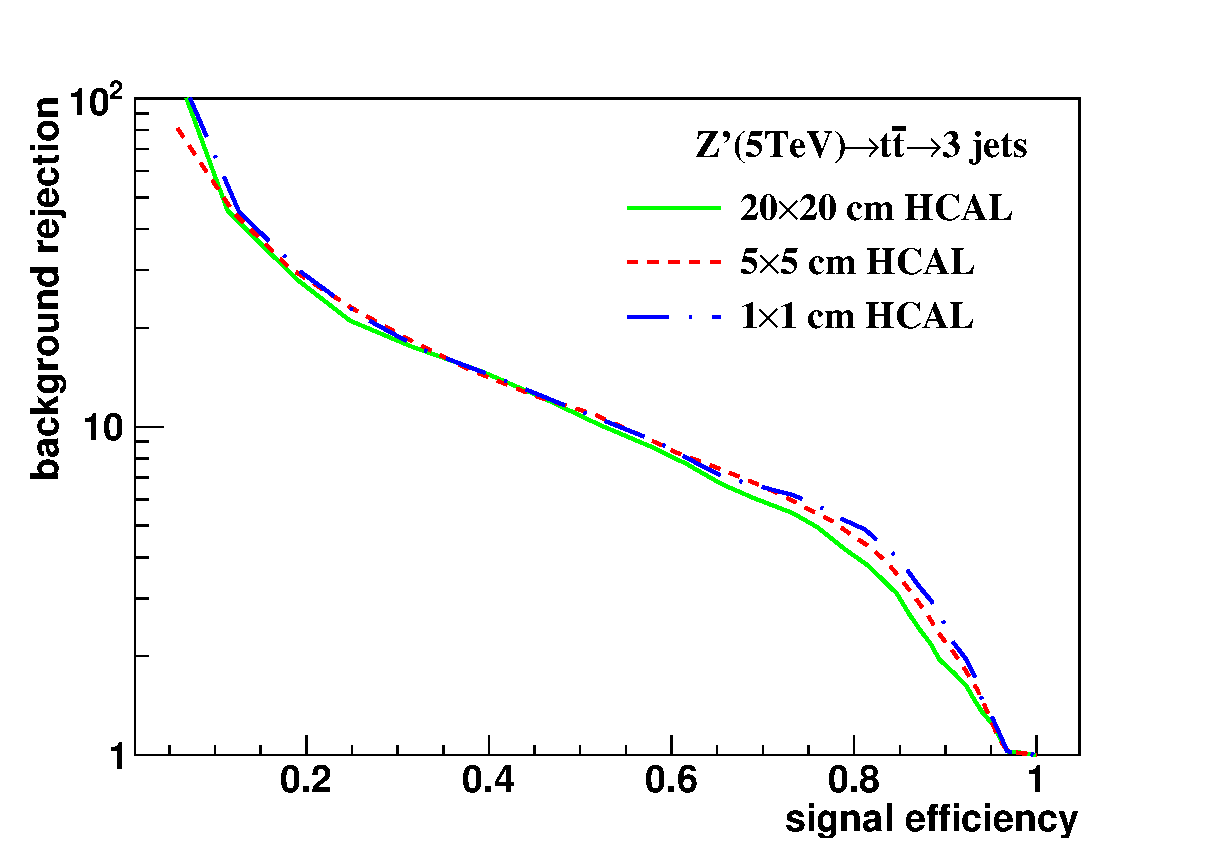
\includegraphics[width=\cmsFigWidth]{figs/A_Cluster_mass_mmdt_5tev_eff_1_central_fix_at_Median_bin_tt_qq_log_no_UOF.eps}
  }
  \subfigure[$M(Z')=10$~TeV] {
  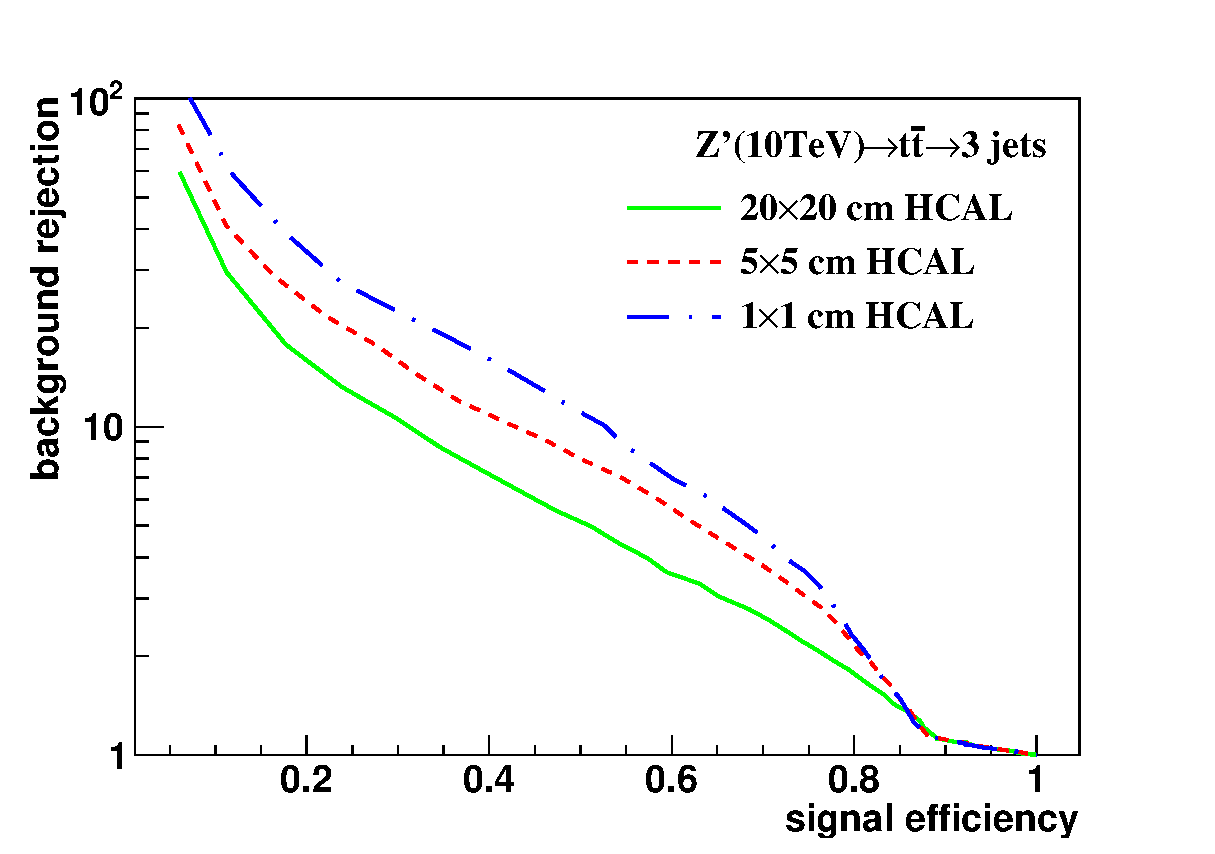
\includegraphics[width=\cmsFigWidth]{figs/A_Cluster_mass_mmdt_10tev_eff_1_central_fix_at_Median_bin_tt_qq_log_no_UOF.eps}
  }\\
 \subfigure[$M(Z')=20$~TeV] {
 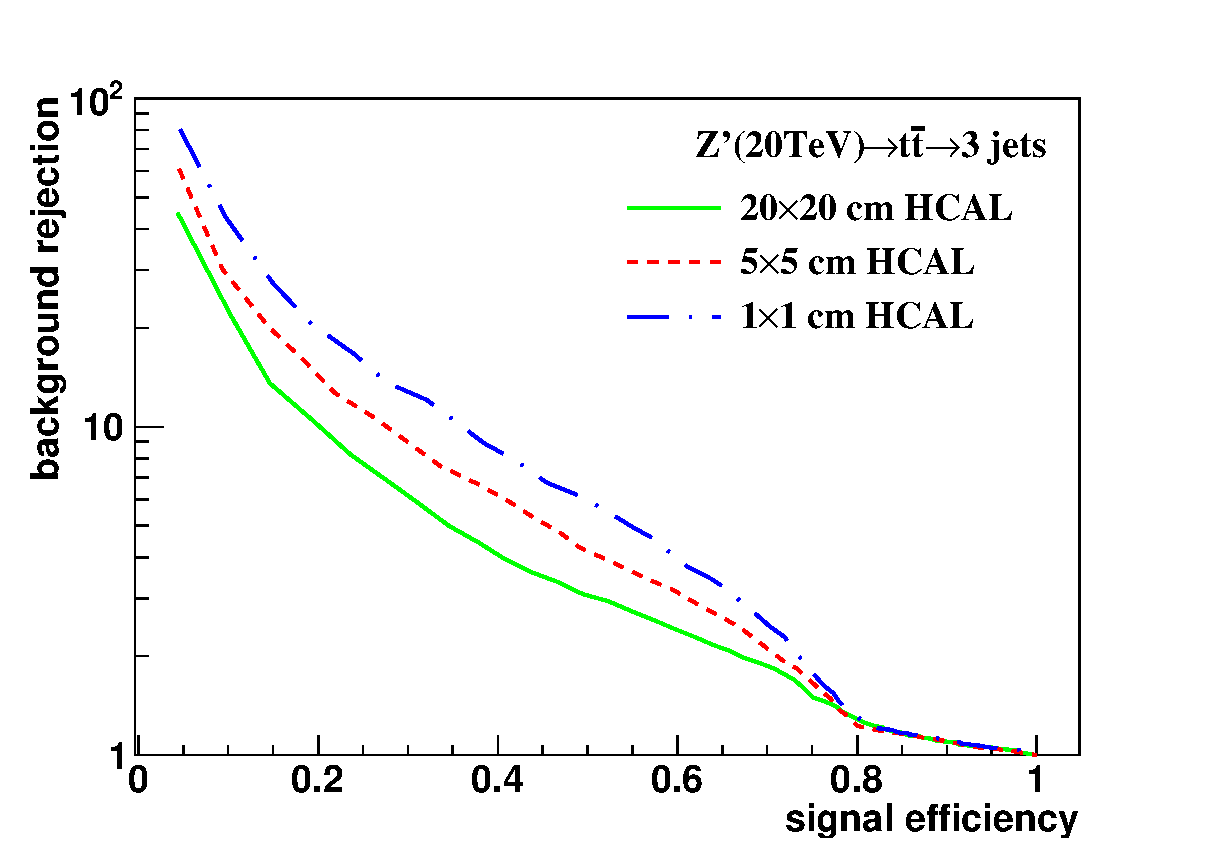
\includegraphics[width=\cmsFigWidth]{figs/A_Cluster_mass_mmdt_20tev_eff_1_central_fix_at_Median_bin_tt_qq_log_no_UOF.eps}
 }
 \subfigure[$M(Z')=40$~TeV] {
 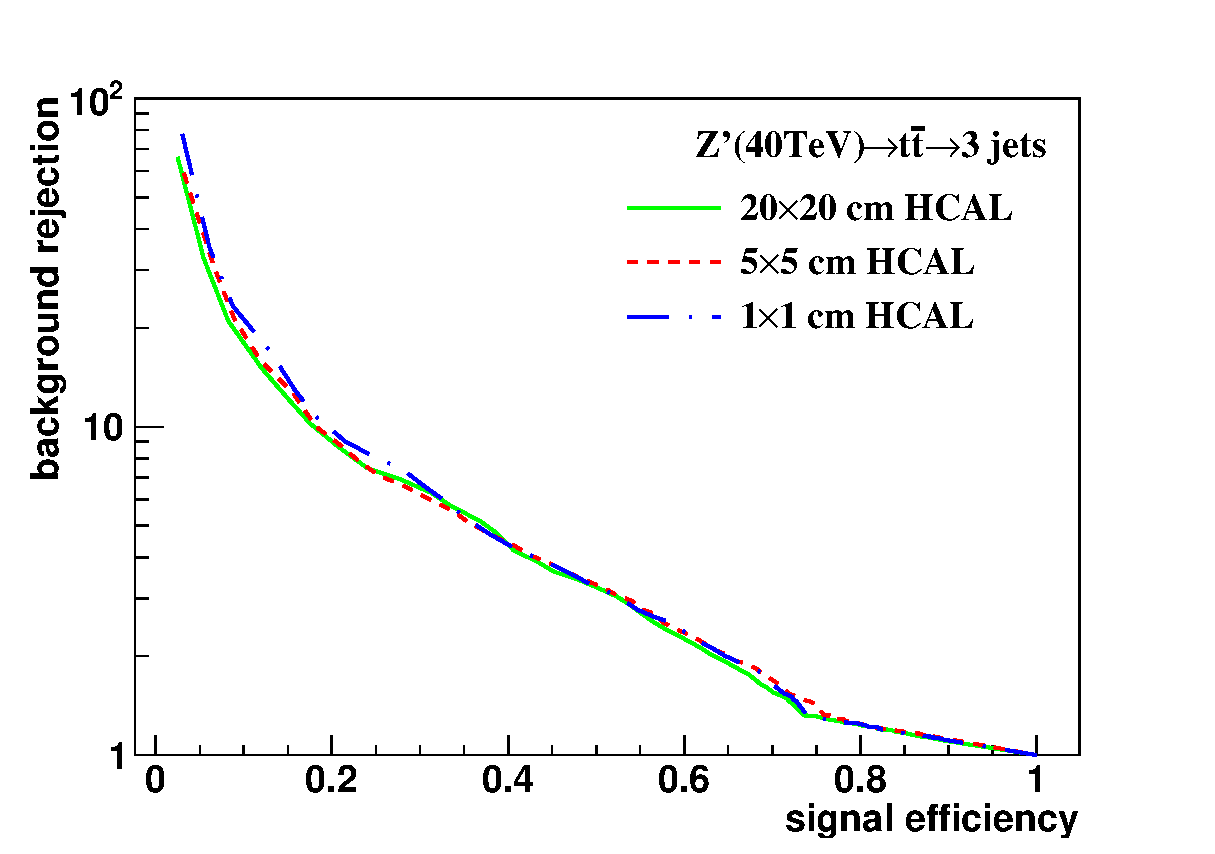
\includegraphics[width=\cmsFigWidth]{figs/A_Cluster_mass_mmdt_40tev_eff_1_central_fix_at_Median_bin_tt_qq_log_no_UOF.eps}
 }
\end{center}
\caption{
The ROC curves of soft drop mass selection for $\beta$=0 
with 5, 10, 20, and 40~TeV c.m. energies. 
Three different detector cell sizes are compared: 20$\times$20, 
5$\times$5, and 1$\times$1 (cm$\times$cm). 
The signal (background) process is Z'$\rightarrow$t$\bar{\mathrm{t}}$
(Z'$\rightarrow$q$\bar{\mathrm{q}}$).
}
\label{fig:cluster_mass_mmdt_tt_ROC}
\end{figure}



\begin{figure}
\begin{center}
   \subfigure[20~TeV at 20$\times$20 (cm$\times$cm) with cluster] {
   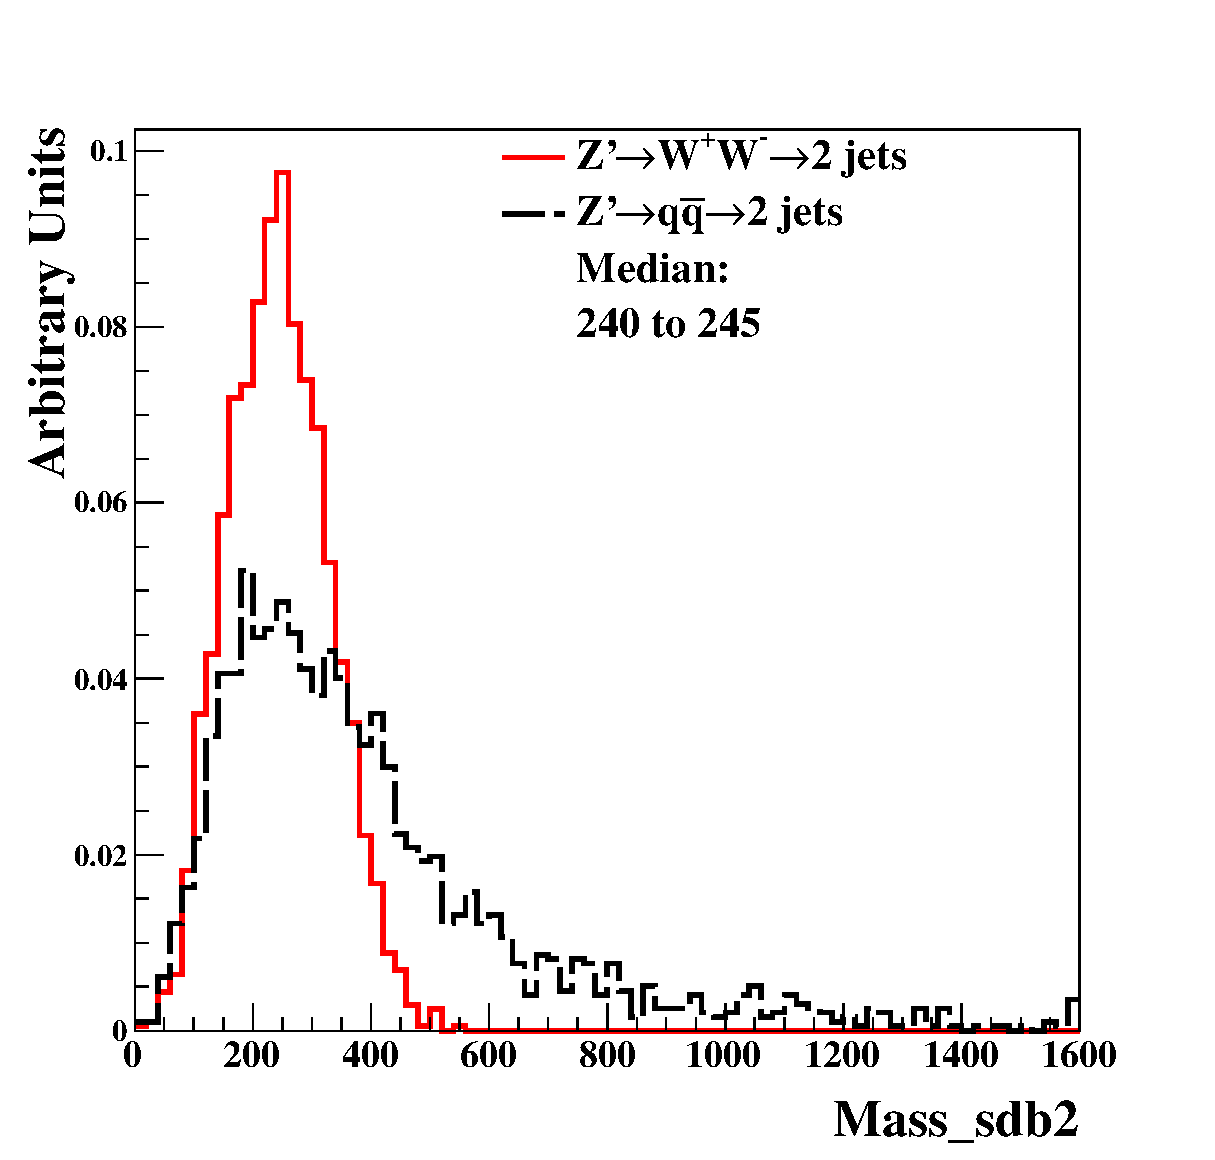
\includegraphics[width=0.25\textwidth]{figs/Dis_cluster_010_mass_sdb2_ww_20tev_04_1600_no_UOF.eps}
   }
    \subfigure[20~TeV at 5$\times$5 (cm$\times$cm) with cluster] {
   \includegraphics[width=0.25\textwidth]{figs/Dis_cluster_009_mass_sdb2_ww_20tev_04_1600_no_UOF.eps}\hfill
   }
   \subfigure[20~TeV at 1$\times$1 (cm$\times$cm) with cluster] {
   \includegraphics[width=0.25\textwidth]{figs/Dis_cluster_012_mass_sdb2_ww_20tev_04_1600_no_UOF.eps}\hfill
   }
\end{center}
\caption{
Distributions of soft drop mass for $\beta$=2, with 5, 10, 20, and 
40~TeV c.m. energies and three different detector cell sizes: 20$\times$20, 
5$\times$5, and 1$\times$1 (cm$\times$cm). The signal (background) process is 
Z'$\rightarrow$WW (Z'$\rightarrow$q$\bar{\mathrm{q}}$).
}
\label{fig:cluster_mass_sdb2_ww}
\end{figure}


\begin{figure}
\begin{center}
  \subfigure[$M(Z')=5$~TeV] {
  \includegraphics[width=\cmsFigWidth]{figs/A_Cluster_mass_sdb2_5tev_eff_1_central_fix_at_Median_bin_ww_qq_log_no_UOF.eps}
  }
  \subfigure[$M(Z')=10$~TeV] {
  \includegraphics[width=\cmsFigWidth]{figs/A_Cluster_mass_sdb2_10tev_eff_1_central_fix_at_Median_bin_ww_qq_log_no_UOF.eps}
  }\\
 \subfigure[$M(Z')=20$~TeV] {
 \includegraphics[width=\cmsFigWidth]{figs/A_Cluster_mass_sdb2_20tev_eff_1_central_fix_at_Median_bin_ww_qq_log_no_UOF.eps}
 }
 \subfigure[$M(Z')=40$~TeV] {
 \includegraphics[width=\cmsFigWidth]{figs/A_Cluster_mass_sdb2_40tev_eff_1_central_fix_at_Median_bin_ww_qq_log_no_UOF.eps}
 }
\end{center}
\caption{
The ROC curves of soft drop mass selection for $\beta$=2
with 5, 10, 20, and 40~TeV c.m. energies. 
Three different detector cell sizes are compared: 20$\times$20, 
5$\times$5, and 1$\times$1 (cm$\times$cm). 
The signal (background) process is Z'$\rightarrow$WW 
(Z'$\rightarrow$q$\bar{\mathrm{q}}$).
}
\label{fig:cluster_mass_sdb2_ww_ROC}
\end{figure}


\begin{figure}
\begin{center}
   \subfigure[20~TeV at 20$\times$20 (cm$\times$cm) with cluster] {
   \includegraphics[width=0.25\textwidth]{figs/Dis_cluster_010_mass_sdb2_tt_20tev_04_tt_2400_no_UOF.eps}
   }
   \subfigure[20~TeV at 5$\times$5 (cm$\times$cm) with cluster] {
   \includegraphics[width=0.25\textwidth]{figs/Dis_cluster_009_mass_sdb2_tt_20tev_04_tt_2400_no_UOF.eps}\hfill
   }
   \subfigure[20~TeV at 1$\times$1 (cm$\times$cm) with cluster] {
   \includegraphics[width=0.25\textwidth]{figs/Dis_cluster_012_mass_sdb2_tt_20tev_04_tt_2400_no_UOF.eps}\hfill
   }
\end{center}
\caption{
Distributions of soft drop mass for $\beta$=2, with 5, 10, 20, and 
40~TeV c.m. energies and three different detector cell sizes: 20$\times$20, 
5$\times$5, and 1$\times$1 (cm$\times$cm). The signal (background) process is 
Z'$\rightarrow$t$\bar{\mathrm{t}}$ (Z'$\rightarrow$q$\bar{\mathrm{q}}$).
}
\label{fig:cluster_mass_sdb2_tt}
\end{figure}


\begin{figure}
\begin{center}
  \subfigure[$M(Z')=5$~TeV] {
  \includegraphics[width=\cmsFigWidth]{figs/A_Cluster_mass_sdb2_5tev_eff_1_central_fix_at_Median_bin_tt_qq_log_no_UOF.eps}
  }
  \subfigure[$M(Z')=10$~TeV] {
  \includegraphics[width=\cmsFigWidth]{figs/A_Cluster_mass_sdb2_10tev_eff_1_central_fix_at_Median_bin_tt_qq_log_no_UOF.eps}
  }
  \\
 \subfigure[$M(Z')=20$~TeV] {
 \includegraphics[width=\cmsFigWidth]{figs/A_Cluster_mass_sdb2_20tev_eff_1_central_fix_at_Median_bin_tt_qq_log_no_UOF.eps}
 }
 \subfigure[$M(Z')=40$~TeV] {
 \includegraphics[width=\cmsFigWidth]{figs/A_Cluster_mass_sdb2_40tev_eff_1_central_fix_at_Median_bin_tt_qq_log_no_UOF.eps}
 }
\end{center}
\caption{
The ROC curves of soft drop mass selection for $\beta$=2
with 5, 10, 20, and 40~TeV c.m. energies. 
Three different detector cell sizes are compared: 20$\times$20, 
5$\times$5, and 1$\times$1 (cm$\times$cm). 
The signal (background) process is Z'$\rightarrow$t$\bar{\mathrm{t}}$
(Z'$\rightarrow$q$\bar{\mathrm{q}}$).
}
\label{fig:cluster_mass_sdb2_tt_ROC}
\end{figure}
%%%===============================C2b1 and Tau21,32 Studies================================%%
\subsection{Studies of signal and background separation using jet substructure variables}
In this section, we study different jet substructure variables and compare their ability to separate signal from background with different detector sizes and c.m. energy using ROC curves.\\

\subsubsection{N-subjettiness}
N-subjettiness[\ref{}] is the detection technique of jet substructure which is applied to identify boosted hadronically-decaying objects under conditions of High C.M energy collision. We used $\tau$ variable to distinguish the number of subjet(s) in a fatjet to separate signal from background with different detector sizes in different C.M. energy condition.\\

\subsubsection{The technic of N-subjettiness}
The formula and the technique are as following:\\
\begin{equation}\label{eq:Nsub_1}
\tau_{N}=\frac{1}{d_{0}}\sum_{k}p_{T,k} min\{\Delta R_{1,k},\Delta R_{2,k},.....\Delta R_{N,k}\}
\end{equation}
\begin{equation}\label{eq:Nsub_2}
d_{0}=\sum_{k}p_{T,k} R_{0}
\end{equation}
k runs over all constituent particles in the given jets (fatjet), $p_{T,k}$ are their transverse momentum, $\Delta R_{J,k}=\sqrt{(\Delta \eta)^{2}+(\Delta \phi)^{2}}$ is the distance between the constituent particles k and the candidate subjet J on the $\eta-\phi$ plane. $R_{0}$ is the characteristic jet radius used in Anti-kt(AK) jet algorithm at starting. $d_{0}$ is the normalization factor.\\

To use this technique, first, Anti-kt(AK) algorithm\ref{} with radius($R_{0}$=0.4 in formula \ref{eq:Nsub_2}) is used to reconstruct jets in the detector. Second, after reconstructing the jets, exclusive $k_{T}$ algorithm[\ref{}] is used to find the jet axis in a fatjet, and applied in calculating the radius from constituent particles to jet axis. Third, start applying the formula [\ref{eq:Nsub_1}], looping all constituent particles in a fatjet. Finally, when finishing running all particles, it will give out $\tau_{N}$, where N is positive integer. 

If a fatjet has exactly N subjet(s), its $\tau_{N}$ is smaller than the $\tau_{N-1}$. It can return the truth that how many subjet(s) there is(are) in a fatjet. In our study, we used $\tau_{21}$=$\tau_{2}$/$\tau_{1}$  and $\tau_{32}$=$\tau_{3}$/$\tau_{2}$ in distinguishing two-subjets fatjet and three-subjets fatjet of signal processes from one-subjet fatjet of background process individually. \\ 

\subsubsection{Analysis method}\label{Analysis_method_for_Tau_C}
Similar with the soft drop mass in section\ref{}, we need to apply some methods to quantify the separation power for different jet substructure variables with different configurations of detector, and figure out the best configuration for distinguishing signal from background. We still applied the ROC curves to be our comparison tools. \\

Before scanning the efficiencies, we first did some pre-selection tasks. Inspired by the paper\ref{}, it pointed out that applying the mass cut would give us the best separation power, so first we selected the optimized mass window.  We did the prerequestion that in the signal events, compare the adjacent bins from the largest number of events iteratively. Until We included the 75\% mass events, we stopped and used the events which were included.\\

Second, inspired by the Pearson lemma, it told us that if we used the ratio of the two histograms to be the window selection for the ROC curves, and it will give us the best solution, so we applied this method in our study. We used $\frac{\mathrm{Signal \ histogram}}{\mathrm{Background \ histogram}}$ of ratio histogram to be our window to draw the ROC curves. Compare the adjacent bins from the bin of most event in ratio histogram, and extended the width with higher side until all bins were included in.\\

\subsubsubsection{Results and conclusion}
In the figure [\ref{fig:Rawhit_05GeV_tau21_Dis}][\ref{fig:Rawhit_05GeV_tau32_Dis}], they show the histograms of $\tau_{21}$ and $\tau_{32}$ with $\sqrt{s} = 20\TeV$ after selecting the events as an example. As a result of figure [\ref{fig:Rawhit_05GeV_tau21_ROC}][\ref{fig:Rawhit_05GeV_tau32_ROC}], they perform the ROC curves of $\tau_{21}$ and $\tau_{32}$ with different detector cell sizes and C.M. energy. The smallest detector cell size(1$\times$1) doesn't have the best separation power to distinguish signal from background. Some of them have the best separation power with the bigger cell size (5$\times$5 and 20$\times$20).\\

\subsubsection{Energy correlation function}
Energy correlation function (ECF) [\ref{}] is another kind of detection technique of jet substurcture that is used to distinguish the number of subjets in a fatjet under high C.M. energy conditions. This method only uses the momenta of particles and the angles between them without additional algorithm.\\
\subsubsubsection{The technic of energy correlation function}
The basic ECF formula is as following:\\
\begin{equation} \label{eq:ECF_Original}
ECF(N,\beta)=\sum_{i_{1}<i_{2}<....<i_{N}\in J} (\prod_{a=1}^{N}P_{ia})(\prod_{b=1}^{N-1}\prod_{c=b+1}^{N} R_{i_{b}i_{c}})^{\beta}
\end{equation}

In the formula \ref{eq:ECF_Original}, the sum loop all particles in the jet $J$ by using the information of $P_{ia}$, which are the momenta of all particles, and $R_{i_{b}i_{c}}$, which are the angles between each particles in the $y$-$\phi$ plane.  in order to use the dimensionless observation to determine whether the number of subjets in system, parameter $\tau_{N}$ is defined as:\\
\begin{equation} \label{eq:ECF_ratio}
\tau_{N}^{(\beta)}\equiv\frac{ECF(N+1,\beta)}{ECF(N,\beta)}
\end{equation}

The idea of formula (\ref{eq:ECF_ratio}) is from N-subjetness, because the behavior of it is very similar to N-subjetness as reference [\ref{}]. In general, if the system has N subjets, $ECF(N+1,\beta)$ should be significantly smaller than $ECF(N,\beta)$, so we can use this advantage to distinguish different number of subjets. Finally, because it is suggested to use $\tau_{21}$=$\tau_{2}$/$\tau_{1}$  and $\tau_{32}$=$\tau_{3}$/$\tau_{2}$, [\ref{}] to distinguish two-subjets fatjet and three-subjets fatjet from one-subjet fatjet in the previous studies, it is also defined as the ratio of $\tau$ there, which is called "Double ratio-ECF" that is used in our study:\\
\begin{equation}
C_{N}^{(\beta)}\equiv\frac{\tau_{N}^{(\beta)}}{\tau_{N-1}^{(\beta)}}=\frac{ECF(N-1,\beta)ECF(N+1,\beta)}{ECF(N,\beta)^2}
\end{equation}

We set N=2 and $\beta=1$ ($C_{2}^{1}$) to distinguish two-subjets fatjet from one-subjet fatjet in our study.

For the analysis method, it is the same as the part \ref{Analysis_method_for_Tau_C}.

\subsubsubsection{The results and conclusion}
In the figure [\ref{fig:Rawhit_05GeV_c2b1_Dis}], they show the histograms of $\tau_{21}$ and $\tau_{32}$ with $\sqrt{s} = 20\TeV$ after selecting the events as an example. For the figure [\ref{fig:Rawhit_05GeV_c2b1_ROC}], they present the ROC curves of $C_{2}^{1}$ with different detector cell sizes and C.M. energy. The smallest detector cell size(1$\times$1) doesn't have the best separation power to distinguish signal from background. In addition, in some cases such like (a), the biggest one (20$\times$20) has the best distinguish power under the same c.m. energy.\\

\subsubsection{Conclusion}
The studies presented in this previous sections show that the reconstruction of jet substructure 
variables for future colliders will benefit from small cell sizes of the hadronic calorimeters. 
This conclusion was obtained using the simulation of calorimeter response combined with reconstruction of 
calorimeter clusters and the Rawhits information used as inputs for jet reconstruction. 
Hadronic calorimeters that used the cell sizes of 20~$\times $~20~cm$^2$ ($\Delta \eta \times \Delta \phi = 0.087\times 0.087$) 
had the worst performance for almost every 
substructure variable which were considered in our analysis, for the resonance mass at $\sqrt{s} = 5\TeV$ to $\sqrt{s} = 20\TeV$. 
Such cell sizes are similar to those used for the ATLAS and CMS detectors at the LHC. 
In out studies, we obtained the performance of a hadronic calorimeter with 
$\Delta \eta \times \Delta \phi = 0.022\times0.022$ ($5 \times 5$~$\mathrm{cm}^2$ cell size) is, in most cases,
better than for a detector with $0.087\times 0.087$ cells.

Thus this study confirms the  HCAL geometry of the SiFCC detector~\cite{Chekanov:2016ppq},
with the $\Delta \eta \times \Delta \phi = 0.022\times0.022$ HCAL cells.
It also confirms the HCAL design of the baseline FCC-hh~\cite{fcc1,fcc2} detector with
$\Delta \eta \times \Delta \phi = 0.025\times0.025$ HCAL cells.
%25bins
\begin{figure}
\begin{center}
   \subfigure[20TeV at 20$\times$20(cm$\times$cm) in 0.5GeV] {
   \includegraphics[width=0.25\textwidth]{figs/Dis_Rawhit_05GeV_010_c2b1_20tev_04_after_cut_Man_25_no_UOF_new_75pa_for_paper.eps}
   }
   \subfigure[20TeV at 5$\times$5(cm$\times$cm) in 0.5GeV] {
   \includegraphics[width=0.25\textwidth]{figs/Dis_Rawhit_05GeV_009_c2b1_20tev_04_after_cut_Man_25_no_UOF_new_75pa_for_paper.eps}
   }
   \subfigure[20TeV at 1$\times$1(cm$\times$cm) in 0.5GeV] {
   \includegraphics[width=0.25\textwidth]{figs/Dis_Rawhit_05GeV_012_c2b1_20tev_04_after_cut_Man_25_no_UOF_new_75pa_for_paper.eps}
   }\end{center}
\caption{Distributions of Mann-Whitney value U in 5, 10, 20, 40TeV energy collision for c2b1 in different detector sizes. Cell Size in 20$\times$20, 5$\times$5, and 1$\times$1(cm$\times$cm) are shown here.}
\label{fig:Rawhit_05GeV_c2b1_Dis}
\end{figure}

\begin{figure}
\begin{center}
   \subfigure[5 TeV using Rawhit 0.5GeV cut method with New2 after cut Method] {
   \includegraphics[width=\cmsFigWidth]{figs/Rawhit_05GeV_c2b1_5tev_eff_1_New2_after_cut_25bins_no_UOF_new_75pa.eps}\hfill
   }
   \subfigure[10 TeV using Rawhit 0.5GeV cut method with New2 after cut Method] {
   \includegraphics[width=\cmsFigWidth]{figs/Rawhit_05GeV_c2b1_10tev_eff_1_New2_after_cut_25bins_no_UOF_new_75pa.eps}
   }\\
   \subfigure[20 TeV using Rawhit 0.5GeV cut method with New2 after cut Method] {
   \includegraphics[width=\cmsFigWidth]{figs/Rawhit_05GeV_c2b1_20tev_eff_1_New2_after_cut_25bins_no_UOF_new_75pa.eps}
   }
   \subfigure[40 TeV using Rawhit 0.5GeV cut method with New2 after cut Method] {
   \includegraphics[width=\cmsFigWidth]{figs/Rawhit_05GeV_c2b1_40tev_eff_1_New2_after_cut_25bins_no_UOF_new_75pa.eps}
   }
\end{center}
\caption{Signal efficiency versus background rejection rate using c2b1.The energies of collision at (a)5, (b)10, (c)20, (d)40TeV are shown here. In each picture, the three ROC curves correspond to different detector sizes.}
\label{fig:Rawhit_05GeV_c2b1_ROC}
\end{figure}



%25bins
\begin{figure}
\begin{center}
   \subfigure[20TeV at 20$\times$20(cm$\times$cm) in 0.5GeV] {
   \includegraphics[width=0.25\textwidth]{figs/Dis_Rawhit_05GeV_010_tau21_20tev_04_after_cut_Man_25_no_UOF_new_75pa_for_paper.eps}
   }
   \subfigure[20TeV at 5$\times$5(cm$\times$cm) in 0.5GeV] {
   \includegraphics[width=0.25\textwidth]{figs/Dis_Rawhit_05GeV_009_tau21_20tev_04_after_cut_Man_25_no_UOF_new_75pa_for_paper.eps}
   }
   \subfigure[20TeV at 1$\times$1(cm$\times$cm) in 0.5GeV] {
   \includegraphics[width=0.25\textwidth]{figs/Dis_Rawhit_05GeV_012_tau21_20tev_04_after_cut_Man_25_no_UOF_new_75pa_for_paper.eps}
   }\end{center}
\caption{Distributions of Mann-Whitney value U in 5, 10, 20, 40TeV energy collision for $\tau_{21}$  in different detector sizes. Cell Size in 20$\times$20, 5$\times$5, and 1$\times$1(cm$\times$cm) are shown here.}
\label{fig:Rawhit_05GeV_tau21_Dis}
\end{figure}
\begin{figure}
\begin{center}
   \subfigure[5 TeV using Rawhit 0.5GeV cut method with New2 after cut Method] {
   \includegraphics[width=\cmsFigWidth]{figs/Rawhit_05GeV_tau21_5tev_eff_1_New2_after_cut_25bins_no_UOF_new_75pa.eps}\hfill
   }
   \subfigure[10 TeV using Rawhit 0.5GeV cut method with New2 after cut Method] {
   \includegraphics[width=\cmsFigWidth]{figs/Rawhit_05GeV_tau21_10tev_eff_1_New2_after_cut_25bins_no_UOF_new_75pa.eps}
   }\\
   \subfigure[20 TeV using Rawhit 0.5GeV cut method with New2 after cut Method] {
   \includegraphics[width=\cmsFigWidth]{figs/Rawhit_05GeV_tau21_20tev_eff_1_New2_after_cut_25bins_no_UOF_new_75pa.eps}
   }
   \subfigure[40 TeV using Rawhit 0.5GeV cut method with New2 after cut Method] {
   \includegraphics[width=\cmsFigWidth]{figs/Rawhit_05GeV_tau21_40tev_eff_1_New2_after_cut_25bins_no_UOF_new_75pa.eps}
   }
\end{center}
\caption{Signal efficiency versus background rejection rate using $\tau_{21}$.The energies of collision at (a)5, (b)10, (c)20, (d)40TeV are shown here. In each picture, the three ROC curves correspond to different detector sizes.}
\label{fig:Rawhit_05GeV_tau21_ROC}
\end{figure}




%25bins
\begin{figure}
\begin{center}
   \subfigure[20TeV at 20$\times$20(cm$\times$cm) in 0.5GeV] {
   \includegraphics[width=0.25\textwidth]{figs/Dis_Rawhit_05GeV_010_tau32_20tev_04_after_cut_Man_25_no_UOF_new_75pa_for_paper.eps}
   }
   \subfigure[20TeV at 5$\times$5(cm$\times$cm) in 0.5GeV] {
   \includegraphics[width=0.25\textwidth]{figs/Dis_Rawhit_05GeV_009_tau32_20tev_04_after_cut_Man_25_no_UOF_new_75pa_for_paper.eps}
   }
   \subfigure[20TeV at 1$\times$1(cm$\times$cm) in 0.5GeV] {
   \includegraphics[width=0.25\textwidth]{figs/Dis_Rawhit_05GeV_012_tau32_20tev_04_after_cut_Man_25_no_UOF_new_75pa_for_paper.eps}
   }
   }\end{center}
\caption{Distributions of Mann-Whitney value U in 5, 10, 20, 40TeV energy collision for $\tau_{32}$  in different detector sizes. Cell Size in 20$\times$20, 5$\times$5, and 1$\times$1(cm$\times$cm) are shown here.}
\label{fig:Rawhit_05GeV_tau32_Dis}
\end{figure}

\begin{figure}
\begin{center}
   \subfigure[5 TeV using Rawhit 0.5GeV cut method with New2 after cut Method] {
   \includegraphics[width=\cmsFigWidth]{figs/Rawhit_05GeV_tau32_5tev_eff_1_New2_after_cut_25bins_no_UOF_new_75pa.eps}\hfill
   }
   \subfigure[10 TeV using Rawhit 0.5GeV cut method with New2 after cut Method] {
   \includegraphics[width=\cmsFigWidth]{figs/Rawhit_05GeV_tau32_10tev_eff_1_New2_after_cut_25bins_no_UOF_new_75pa.eps}
   }\\
   \subfigure[20 TeV using Rawhit 0.5GeV cut method with New2 after cut Method] {
   \includegraphics[width=\cmsFigWidth]{figs/Rawhit_05GeV_tau32_20tev_eff_1_New2_after_cut_25bins_no_UOF_new_75pa.eps}
   }
   \subfigure[40 TeV using Rawhit 0.5GeV cut method with New2 after cut Method] {
   \includegraphics[width=\cmsFigWidth]{figs/Rawhit_05GeV_tau32_40tev_eff_1_New2_after_cut_25bins_no_UOF_new_75pa.eps}
   }
\end{center}
\caption{Signal efficiency versus background rejection rate using $\tau_{32}$.The energies of collision at (a)5, (b)10, (c)20, (d)40TeV are shown here. In each picture, the three ROC curves correspond to different detector sizes.}
\label{fig:Rawhit_05GeV_tau32_ROC}
\end{figure}

\section{Conclusion for all studies}
I have done the "detector traveling" from now to the future within the project time. For now, at the start, I studied the cross-talk on the no sensor-based Hexaboard which will be used in HGCAL. We explored the phenomenon and saw the correlated cross-talk and the anti-correlated cross-talk. Later, we did the project with the HGCAL test-beam results of MC samples to do the e-like pions tagging and rejected them by the cuts and variable we developed. We saw the expected results in the October test-beam MC samples. Last but not least, we came to the future project with the SiFCC detector. By using the different configurations of the detector with the different jet substructure variables and soft-drop mass, to see whether the high granularity could give us the best results to distinguish the signal from background in the SiFCC detector. For our surprise, the smallest configuration is not the best, and we think that it need to be optimized. 

\section{Summary for Milestone Achieved within the project time}
\begin{itemize}
\item Submit my first journal paper: "Studies of granularity of a hadronic calorimeter for tens-of-TeV jets at a 100 TeV $pp$ collider" to arxiv and the Journal of instrumentation(JINST), now is reviewed by the people in the journal.
\item Submit my first conference paper: "Jet Substructure Variables with the SiFCC Detector at 100 TeV" to arxiv and is published by the Journal of Proceeding of Science(PoS).
\item Accepted and report the poster with FCC detector studies in the International Conference of High Energy Physics in 2018(ICHEP2018).
\item Accepted and report the two posters with HGCAL studies and FCC detector studies in the Taiwan Physics Society(TPS) annual meeting in 2019. 
\end{itemize}

\section{Acknowledgement}
First, thanks for my supervisors, Prof.Shin-Shan Eiko Yu from NCU, Prof.Ashtusoh from Duke University and Prof.Stathes Paganis, Prof.Rong-Shayang Lu from NTU, without them, I can't do those good studies smoothly, and publish the results well. Also, I would like to thanks LHC-CMS, NCU and NTU to give me the resource, including the data, hardware and the server resource, to study my interested topics. And thanks for all people in NCUHEP, NTUHEP groups who have helped me. Last but not least, I'm glad to thanks MOST to support me to do this studies. 













































\begin{comment}

\section{Summary for Milestone Achieved within the project time}
\begin{itemize}
\item Submit my first journal paper: "Studies of granularity of a hadronic calorimeter for tens-of-TeV jets at a 100 TeV $pp$ collider" to arxiv and the Journal of instrumentation(JINST), now is reviewed by the people in the journal.
\item Submit my first conference paper: "Jet Substructure Variables with the SiFCC Detector at 100 TeV" to arxiv and is published by the Journal of Proceeding of Science(PoS).
\item Accepted and report the poster with FCC detector studies in the International Conference of High Energy Physics in 2018(ICHEP2018).
\item Accepted and report the two posters with HGCAL studies and FCC detector studies in the Taiwan Physics Society(TPS) annual meeting in 2019. 
\end{itemize}





\begin{figure}[!htb]
\centering
     \includegraphics[width=\cmsFigWidth]{PCB_study/HG_Chip0_channel18_Pedestal_TS4_Subtract_mean_and_RMS.pdf}
     \includegraphics[width=\cmsFigWidth]{PCB_study/HG_Chip0_channel22_Pedestal_TS4_Subtract_mean_and_RMS.pdf}\\
     \includegraphics[width=\cmsFigWidth]{PCB_study/HG_Chip0_channel44_Pedestal_TS4_Subtract_mean_and_RMS.pdf}
     \includegraphics[width=\cmsFigWidth]{PCB_study/HG_Chip0_channel52_Pedestal_TS4_Subtract_mean_and_RMS.pdf}
\caption{These figures present the correlation between the different DAQ input and Pedestal-subtracted mean and error. The Top left and right pictures perform the channel of 18 and 22, which are closed to the injection channel. The down left and right pictures show channel of 44 and 52, which are farther from the injection channel.}
\label{fig:PCB_injection_pulse_study}
\end{figure}

\subsection{The results of application with October test-beam MC}

 it shows the $E_{10}$ plot which is drawn by the events which are passed all cut we told before.
\section{Milestone Achieved}
\begin{itemize}
\item Submit my first journal paper: "Studies of granularity of a hadronic calorimeter for tens-of-TeV jets at a 100 TeV $pp$ collider" to arxiv and the Journal of instrumentation(JINST), now it is reviewed by the people in the journal.
\item Submit my first conference paper: "Jet Substructure Variables with the SiFCC Detector at 100 TeV" to arxiv and it is publised by the Journal of Proceeding of Science(PoS).
\item Accepted and report the poster with FCC detector studies in the International Conference of High Energy Physics in 2018(ICHEP2018).
\item Accepted and report the two posters with HGCAL studies and FCC detector studies in the Taiwan Physics Society(TPS) annual meeting in 2019. 
\end{itemize}

\section{Pion-rejection studies with a CMS HGCAL test-beam prototype ECAL}







\section{Acknowledgement}
First, thanks for my supervisors, Prof.Shin-Shan Eiko Yu from NCU, Prof.Ashtusoh from Duke University and Prof.Stathes Paganis, Prof.Rong-Shayang Lu from NTU, without them, I can't do those good studies smoothly, and publish the results well. Also, I would like to thanks LHC-CMS, NCU and NTU to give me the resource, including the data, hardware and the server resource, to study my interested topics. And thanks for all people in NCUHEP, NTUHEP groups who have helped me. Last but not least, I'm glad to thanks MOST to support me to do this studies. 


Hypotheses for physics beyond the standard model (SM) predict the existence of heavy resonances that decay to any combination of two among 
the massive vector bosons (W or Z, collectively referred to as V) or to a V and the scalar SM Higgs boson (H). Among the considered models 
are those dealing with warped extra dimensions (WED)~\cite{Randall:1999ee,Randall:1999vf} and 
composite-Higgs bosons~\cite{Bellazzini:2014yua,CHM2,Composite2,Greco:2014aza}. 
The benchmark models considered are a heavy vector triplet (HVT) model~\cite{Pappadopulo:2014qza} and the bulk 
scenario~\cite{Agashe:2007zd, Fitzpatrick:2007qr, Antipin:2007pi} ($\Gbulk$ graviton) in the Randall--Sundrum (RS) WED 
model~\cite{Randall:1999ee,Randall:1999vf}.
The HVT model generalizes a large number of models that predict spin-1 resonances, such as those in composite-Higgs theories, which can 
arise as a singlet, either \PWpr or \PZpr~\cite{Grojean:2011vu,Langacker:2008yv,Salvioni:2009mt}, or as a $\Vprime$ triplet 
(where $\Vprime$ represents $\PWpr$ and $\PZpr$ bosons)~\cite{Pappadopulo:2014qza}.
The HVT and $\Gbulk$ models are considered as benchmarks for diboson resonances with spin~1 
($\PWpr\to\PW\Z$ or WH, $\PZpr\to\PW\PW$ or ZH), and spin~2 ($\Gbulk\to\PW\PW$ or ZZ), respectively, produced via quark-antiquark 
annihilation ($\qqbarpr\to\PWpr$, $\qqbar\to\PZpr$) and gluon-gluon fusion ($\Pg\Pg\to \Gbulk$).

This analysis presents a search for resonances with masses above 0.6\TeV decaying into a pair of vector bosons.
The analysis is based on data collected in proton-proton collisions at $\sqrt{s} = 13\TeV$ with the CMS experiment at the CERN LHC during 
2015, corresponding to an integrated luminosity of 2.3 and 2.7\fbinv for the $\ell\Pgn\qqbar$, where $\ell=\Pgm$ or e, and $\qqbar\qqbar$ 
final state, respectively. The \lnujet{} search also includes the $\PW\to\Pgt\Pgn$ contribution from the decay $\Pgt\to\ell\Pgn\Pagn$. 
The gain in sensitivity from $\Pgt$ leptons is limited by the small branching fractions involved. The key challenge of the analyses is the 
reconstruction of the highly energetic decay products. Since the resonances under study have masses of order 1\TeV, their decay products, 
\ie{} the bosons, have on average transverse momenta (\pt) of several hundred GeV or more. As a consequence, the particles emerging from 
the boson decays are very collimated. In particular, the jet-decay products of the bosons cannot be resolved using the standard algorithms, 
but are instead reconstructed as a single jet object. Dedicated techniques, called jet ``V tagging'' techniques, are applied to exploit the 
substructure of such objects, to help resolve jet decays of massive bosons~\cite{CMS-PAS-JME-14-002,Khachatryan:2014vla}. The V tagging 
also helps suppress SM backgrounds, which mainly originate from the production of multijet, W+jets, and nonresonant VV events.

The final states considered are either $\ell\Pgn\qqbar$ or $\qqbar\qqbar$, where the hadronic decay products of the V decay are
reconstructed in a single jet. They result in events with either a charged lepton, a neutrino, and a single reconstructed jet (\lnujet{} 
channel), or two reconstructed jets (dijet channel). As in the analyses of previous data~\cite{Khachatryan:2014gha, Khachatryan:2014hpa}, 
the aim is to reconstruct all decay products of the new resonance to be able to search for a localized enhancement in the diboson invariant 
mass spectrum. While the analyses in general aim at large resonance masses, we conduct two exclusive searches in the \lnujet{} final state, 
separately optimized for the mass ranges 0.6--1.0\TeV (``low-mass'') and $> 1$\TeV (``high-mass'').

The AK8 jets are used to reconstruct the W jet and Z jet candidates from their decays to highly boosted quark jets. To discriminate against m\
ultijet backgrounds, we exploit both the reconstructed jet mass, which is required to be close to the W or \Zo boson mass, and the two-prong \
jet substructure produced by the particle cascades of two high-\pt quarks that merge into one jet~\cite{Khachatryan:2014vla}. Jets that are i\
dentified as arising from the merged decay products of a V boson are hereafter referred to as ``V jets''.


As a first step in exploring potential substructure, the jet constituents are subjected to a jet grooming algorithm that improves the resolut\
ion in the jet mass and reduces the effect of pileup~\cite{Chatrchyan:2013vbb}.
The goal of the algorithm is to recluster the jet constituents, while applying additional requirements that eliminate soft, large-angle QCD r\
adiation
that increases the jet mass relative to the initial V boson mass. Different jet grooming algorithms have been explored at CMS, and their perf\
ormance on jets in multijet processes has been studied in detail~\cite{Chatrchyan:2013vbb}.
In this analysis, we use the \textit{jet pruning}~\cite{jetpruning1,Ellis:2009me} algorithm for the main analysis and the \textit{jet trimmin\
g} algorithm~\cite{Krohn:2009th} at the trigger level as well as for cross checks.
Jet pruning reclusters each AK8 jet starting from all its original constituents, through the implementation of the Cambridge-Aachen (CA) algo\
rithm~\cite{Catani:1993hr,Dokshitzer:1997in} to discard ``soft'' recombinations in each step of the iterative CA procedure.
The pruned jet mass, \mJ{}, is computed from the sum of the four-momenta of the constituents that are not removed by the pruning; it is then \
scaled by the same factor as that used to correct the original jet \pt. The jet is considered as a V jet candidate if \mJ{} falls in the rang\
e $\SRLOW < \mJ < \SRHIGH\GeV$, which we define as the signal jet mass window. In the low-mass analysis, only W jet candidates are considered\
, thus the mass window applied is $65 < \mJ < 95\GeV$.

Additional discrimination against jets from gluon and single-quark hadronization is obtained from the quantity called \textit{N-subjettiness}\
~\cite{Thaler:2010tr}. The constituents of the jet before the pruning procedure are reclustered using the \kt algorithm~\cite{Catani:1993hr,E\
llis:1993tq}, until $N$ joint objects (\textit{subjets}) remain in the iterative combination procedure of the algorithm. The $N$-subjettiness\
, $\tau_{N}$, is then defined as
\begin{equation}
\tau_N = \frac{1}{d_{0}} \sum_{k} p_{\mathrm{T},k} \min( \Delta R_{1,k}, \Delta R_{2,k},\ldots,\Delta R_{N,k}),
\end{equation}
where the index $k$ runs over the PF constituents of the jet, and the distances $\Delta R_{n,k}$ are calculated relative to the axis of the $\
n$-th subjet.
The normalization factor $d_{0}$ is calculated as $d_{0}=\sum_{k} p_{\mathrm{T},k}R_{0}$, setting $R_{0}$ to the distance parameter used in t\
he clustering of the original jet.
The variable $\tau_{N}$ quantifies the compatibility of the jet clustering with the hypothesis that exactly $N$ subjets are present, with sma\
ll values of $\tau_{N}$ indicating greater compatibility.
The ratio between 2-subjettiness and 1-subjettiness, $\nsubj=\tau_{2}/\tau_{1}$, is found to be a powerful discriminant between jets originat\
ing from hadronic V decays and from gluon and single-quark hadronization.
Jets from W or \Zo decays in signal events are characterized by lower values of $\nsubj$ relative to SM backgrounds.
We reject V jet candidates with $\nsubj>0.75$. The remaining events are further categorized according to their value of \nsubj{} to enhance t\
he sensitivity of the analysis.

Since data/simulation discrepancies in the jet substructure variables $\mJ$ and $\nsubj$ can bias the signal
efficiency estimated from simulated samples, the modelling of signal efficiency is cross-checked in a signal-free
sample with jets having characteristics that are similar to those expected for a genuine signal.
A sample of high-\pt W bosons that decay to quarks, and are reconstructed as single AK8 jets, is studied in \ttbar and single top quark event\
s.
Scale factors for the $\nsubj{}$ selection efficiency are extracted following Ref.~\cite{Khachatryan:2014vla}.
In this method, the pruned jet mass distributions of events that pass and fail the $\nsubj$ selection are fitted simultaneously to separate t\
he W boson signal from the combinatorial components in the top quark enriched sample in both data and simulation.
The scale factors are used to correct the total signal efficiency and the VV backgroun\
d normalization predicted by the simulation.
The uncertainties in the scale factors quoted for the $\nsubj$ selection include two systematic uncertainties. One comes from the modelling o\
f the nearby jets and \pt spectrum in \ttbar MC events, obtained by comparing LO and NLO \ttbar simulation. The other is due to the choice of\
 the models used to fit signal and background. The quadratic sum of these systematic uncertainties is found to be smaller than half of the st\
atistical uncertainty in the scale factor.
An additional uncertainty is calculated to account for the extrapolation of the scale factor from \ttbar events with an average jet $\pt\appr\
ox200\GeV$ to higher momenta. This is estimated from the difference between \PYTHIA{} and \HERWIG{++}~\cite{Bahr:2008pv} showering  models wi\
th resulting factors of
$4.5\% \ln (\pt/200\GeV)$
and $5.9\%  \ln (\pt/200\GeV)$
for $\tau_{21} < 0.6$ and $\tau_{21} < 0.45$, respectively.
For the $0.45<\tau_{21}<0.75$ selection, this uncertainty is increased by the ratio of the uncertainties in the scale factors,
and treated as anti-correlated with the uncertainty for $\tau_{21}<0.45$.
The mean $\langle\mJ\rangle$ and resolution $\sigma$ value of the Gaussian component of the fitted W jet mass are also extracted to obtain co\
rrections that are applied to the simulated pruned jet mass.
The mass peak position is slightly shifted relative to the W boson mass because of the extra energy deposited in the jet cone from pileup, un\
derlying event, and initial-state radiation not completely removed in the jet pruning procedure. For events with top quarks, additional energ\
y contributions arise also from the possible presence of a b jet close to the W jet candidate.
Because the kinematic properties of W jets and Z jets are very similar, the same corrections are also used when the V jet is assumed to arise\
 from a \Zo boson.


The $\mVV$ distribution observed in data is dominated by SM background processes where single quark or gluon jets are falsely identified as V\
 jets. Depending on the final state, the dominant processes are multijets (dijet channel) and inclusive W boson production (\lnujet channel).\
 Subdominant backgrounds include \ttbar, single top quark, and nonresonant diboson SM production.

In the \lnujet channel, the multijet background is predicted to be negligible from MC simulation, whereas it represents the major contributio\
n in the dijet analysis.
For the latter, we assume that the SM background can be described by a smooth, parametrizable, monotonically decreasing distribution.
The search is performed by separately fitting the background function to each search region
and simultaneously adding resonant Breit--Wigner (BW) forms across all search regions to represent the signal.
The background probability function is defined by empirical functional forms of 3 and 2 parameters, respectively:
\begin{align}
\label{eq:dijet1}
\frac{\rd N}{\rd\mjj}= \frac{ P_0(1-\mjj/\sqrt{s})^{P_1} } { (\mjj/\sqrt{s})^{P_2} }&&\text{and}
&&
\frac{\rd N}{\rd\mjj}= \frac{ P_0 } { (\mjj/\sqrt{s})^{P_2} },
\end{align}
where
\mjj{} is the dijet invariant mass (equivalent to the diboson candidate mass \mVV{} for this channel),
$\sqrt{s}$ is the pp collision energy in the centre of mass,
$P_0$ is a normalization parameter,
and $P_1$ and $P_2$ parametrize the shape of the \mVV{} distribution.
Starting from the two-parameter functional form, a Fisher F-test is used to check at 10\% confidence level (CL)
if additional parameters are needed to model the background distribution. For the WW
categories and the WZ HP category, the two-parameter form is found to describe the data
spectrum sufficiently well, while for all other channels the three-parameter functional form is preferable.
Alternative parametrizations and functions with up to five parameters are also studied as a cross-check.

The backgrounds from \ttbar and single top quark production in the \lnujet{} channel are estimated from data-based correction factors in the \
normalization of the simulation.
A top quark enriched control sample is selected by applying all the analysis requirements in \lnujet{} events
except that the b jet veto is inverted by requiring, instead, at least one b-tagged AK4 jet in the event.
From the comparison between data and simulation, normalization correction factors for \ttbar and single top quark background processes are ev\
aluated in the pruned jet mass regions $65 < \mJ < 105\GeV$ and $65 < \mJ < 95\GeV$, for the electron and muon channels, and for the low- and\
 high-mass selections, separately.
The scale factors include both the W boson signal and the combinatorial components mainly due\
 to events where the extra b jet from the top quark decay is in the proximity of the W, and are used to correct the normalization of the \ttb\
ar and single top quark simulated background predictions in the signal regions.

The W+jets background in the \lnujet channel is estimated through the \emph{$\alpha$ ratio method}.
This method assumes that the correlation between \mJ{} and \mVV{} for the dominant W+jets background can be adequately modelled by simulation\
.
A signal-depleted control region (sideband) is defined by requiring the mass of the V jet to lie below or above the nominal selection; the \m\
VV{} distribution observed in this region is then extrapolated to the nominal region through a transfer function estimated from simulation. O\
ther minor sources of background, such as \ttbar, single top quark, and SM diboson production, are estimated from simulation after applying c\
orrection factors based on control regions in data. The sideband region is defined around the jet mass window. The lower and Top sidebands correspond to t\
he \mJ{} ranges \LOWSBLOW--\SRLOW and \HIGHSBLOW--\HIGHSBHIGH{\GeV}, respectively. The Higgs boson mass region, defined by the range \SRHIGH-\
-\HIGHSBLOW{\GeV}, corresponds to the signal region of searches for diboson in final states with highly Lorentz-boosted Higgs 
bosons~\cite{Khachatryan:2016cfx}, and is therefore not used to estimate the background.

\par The overall normalization of the W+jets background in the signal region is determined from a fit to the \mJ{} distribution in the lower \
and Top sidebands of the data. The analytical form of the fitting function is chosen from simulation studies, as are the contributions from\
 minor backgrounds. 

The \mVV{} distribution observed in data and the
SM background prediction are compared to check for the presence of a
new resonance decaying to vector bosons.
No bins with an excess with significance larger than three standard deviations are observed.
We set Top limits on the
production cross section of such resonances by combining the event categories of
the dijet and \lnujet analyses.
We follow the asymptotic approximation~\cite{AsymptCLs} of the $\mathrm{CL_S}$ criterion described in Refs.~\cite{CLs1,Junk:1999kv}.
The limits computed following this approach are found to agree with the results obtained using the modified frequentist 
prescription~\cite{CLs1,Junk:1999kv}.
For each channel and each signal hypothesis a likelihood function is built from the reconstructed \mVV mass distribution observed in data, 
the background prediction, and the
signal resonance shape. A maximum-likelihood fit to the data is then performed to obtain the best estimate of the signal cross section.
Systematic uncertainties are profiled~\cite{Aad:2015zhl} as log-normal nuisance parameters in the statistical interpretation,
and for each possible value of the fitted signal cross section they are all refitted to maximize the likelihood.

Exclusion limits are set in the context of the bulk graviton model and of the HVT Models A and B,
under the assumption of a natural width negligible compared to the
experimental resolution (narrow-width approximation).
To maximize the sensitivity of the search we combine the results from all the analysis channels
in each of the considered signal hypotheses. In the combination, the systematic uncertainties in jet momentum scale and resolution, V tagging\
 efficiency scale factors, and integrated luminosity are assumed to be 100\% correlated.

\begin{figure}[!htb]
\centering
     \includegraphics[width=\cmsFigWidth]{B2G-16-004/Figure_006-a.pdf}
     \includegraphics[width=\cmsFigWidth]{B2G-16-004/Figure_006-b.pdf}\\
     \includegraphics[width=\cmsFigWidth]{B2G-16-004/Figure_006-c.pdf}
     \includegraphics[width=\cmsFigWidth]{B2G-16-004/Figure_006-d.pdf}
\caption{Observed (black solid) and expected (black dashed) 95\% CL Top limits on the production of a narrow-width resonance decaying to
a pair of vector bosons for different signal hypotheses. In the Top plots, limits are set in the context of a spin-1 neutral \PZpr (left) a\
nd charged \PWpr (right)
resonances, and compared with the prediction of the HVT Models A and B. In the lower left plot, limits are set in the same model under the tr\
iplet hypothesis (\PWpr and \PZpr).
In the lower right plot, limits are set in the context of a bulk graviton with $\ktilde =0.5$ and compared with the prediction.
For $\mathrm{G}_\text{bulk}$, \PZpr and triplet signals (W' signal) with masses $<$0.8\TeV ($<$0.75\TeV), the limits are obtained from the lo\
w-mass \lnujet channel, while for the higher masses they are obtained from the high-mass \lnujet and dijet channels.
}
\label{fig:limitCombined}
\end{figure}


Figure~\ref{fig:limitCombined} shows the resulting expected and observed
exclusion limits at 95\% CL on the signal cross section as a function of the resonance mass for all signal hypotheses.
The limits are compared with the product of cross section and branching fraction ($\sigma\mathcal{B}$) to $\Wo\Wo$ and $\Zo\Zo$
for a bulk graviton with $\ktilde = 0.5$, and with $\sigma\mathcal{B}$ for $\Wo\Zo$ and $\Wo\Wo$ for spin-1 particles predicted by the HVT Mo\
dels A and B.
In this context, we consider a scenario where we expect the \PWpr and \PZpr bosons to be degenerate in mass (triplet hypothesis).
In addition, we consider also a scenario where only a charged (\PWpr) or a neutral (\PZpr) resonance is expected at a given mass (singlet hyp\
othesis).
Combining the analyses leads to about 10--30\% more stringent expected Top limits on the cross section compared
to the most sensitive individual channel, depending on the resonance mass and the signal hypothesis.
For $\mathrm{G}_\text{bulk}$, \PZpr and triplet signals (W' signal) with masses $<$0.8\TeV ($<$0.75\TeV), the limits are obtained from the lo\
w-mass \lnujet channel, while for the higher masses they are obtained from the high-mass \lnujet and dijet channels.
The dijet analysis provides more stringent expected Top limits on the cross sections than the \lnujet{} analysis for resonance masses above\
 1.7\TeV for \PZpr and $>$1.3\TeV for \PWpr, because of the larger branching fractions: $\mathcal{B}(\Wo\Wo\to\qqbar\qqbar) = 44\%$, $\mathca\
l{B}(\Wo\Wo\to\ell\Pgn\qqbar) = 31\%$, $\mathcal{B}(\Wo\Zo\to\qqbar\qqbar) = 46\%$, and $\mathcal{B}$($\Wo\Zo\to\ell\Pgn\qqbar$) = 16\%. In f\
act, the combination of high- and low-purity categories, together with the weak dependence of tagging efficiency on \pt~\cite{CMS-PAS-JME-14-\
002} improves the sensitivity for most potential signal models.
In the narrow-width bulk graviton model, the combined sensitivity of the searches is
not large enough to set mass limits, however, cross sections are excluded in the range 3--1200\unit{fb}.
For HVT Model A (B), the combined data exclude singlet \PWpr resonances with masses $<$2.0~(2.2)\TeV and \PZpr resonances with masses below $\
<$1.6~(1.7)\TeV.
Under the triplet hypothesis, spin-1 resonances with masses $<$2.3 and $<$2.4\TeV are excluded for HVT Models A and B, respectively.

Figure~\ref{fig:hvtscan} shows a scan of the coupling parameters and the corresponding observed 95\% CL exclusion
contours in the HVT model for the combined analyses. The parameters
are defined as $g_{\PV}c_\mathrm{H}$ and $g^2c_\mathrm{F}/g_{\PV}$,  related to the coupling strengths of the new resonance to
the Higgs boson and to fermions. The range of the scan is limited by the assumption that the
new resonance is narrow.  A contour is overlaid, representing the region where the theoretical
width is larger than the experimental resolution of the searches, and hence where the narrow-resonance assumption is not satisfied.
This contour is defined by a predicted resonance width of 5\%, corresponding to the narrowest resonance mass resolution of the searches.

\begin{figure}[!htb]
\centering
     \includegraphics[width=\cmsFigWidth]{B2G-16-004/Figure_007.pdf}
\caption{
Exclusion regions in the plane of the HVT couplings ($g^2c_\mathrm{F}/g_{\PV},g_{\PV}c_\mathrm{H}$) for three
resonance masses, 1.5, 2.0, and 3.5\TeV. Model points A and B of the benchmarks used in the analysis are also shown.
The solid, dashed, and dashed-dotted lines represent the boundaries of the regions excluded by this search for different resonance masses (th\
e region outside these lines is excluded).
The areas indicated by the solid shading correspond to
regions where the resonance width is predicted to be more than 5\% of the resonance mass and
the narrow-resonance assumption is not satisfied.}
\label{fig:hvtscan}
\end{figure}



%%%%%%%%%%%%%%%%%%%%%%%%%%%%%%%%%%%%%%%%%%%%%%%%%%%%%%%%%%%%%%%%%%%%%%%%%%%%%%%
\section{Search for heavy resonances decaying into a vector boson and a Higgs boson in the (ll, lnu, nunu) bb final state at $\sqrt{s}=13~\TeV$\label{sec:vh}}

The contribution of the group of Prof. Yu to this analysis includes the following:
\begin{itemize}
\item Optimization of the pruned Higg-mass selection
\item Optimization of the lepton \pt, \eta, $\Delta \eta$, $\Delta \phi$ selection
\item Generation of the signal simulation
\item Generation of the background simulation to cover the high \pt range
\item Estimation of the systematic uncertainty on the Higgs-tagging signal efficiency due to the use of different parton showering
\item Estimation of the systematic uncertainty due to fit bias
\end{itemize}
Within the group, the major contributors are Prof. Shin-Shan Yu, Dr. Vieri Candelise, Dr. Raman Khurana, the PhD student Yu-Hsiang Chang, and the master students Ching-Wei Chen, Jun-Yi Wu, and Henry Yee-Hsian Tong. The 2015 analysis results were pubishled in Phys Lett. B~\cite{Khachatryan:2016cfx}. I will briefly summarize the analysis below.

The discovery of a Higgs boson \h at the CERN LHC~\cite{bib:Aad20121,bib:Chatrchyan201230,Chatrchyan:2013lba} suggests that the standard 
model (SM) mechanism that connects electroweak (EW) symmetry breaking to the generation of particle masses is largely correct.
However, the relatively light value of the Higgs boson mass 
$\mH = 125.09 \pm 0.21\stat \pm 0.11\syst\GeV$~\cite{Aad:2014aba,Khachatryan:2014jba,Chatrchyan:2014vua,Aad:2015zhl} leaves the hierarchy 
problem unsolved~\cite{1988NuPhB}, pointing to phenomena beyond the SM, which could be unveiled by searches at the LHC.
Many theories that incorporate phenomena beyond the SM postulate the existence of new heavy resonances coupled to the SM bosons. 
Among them, weakly coupled spin-1 $\PZpr$~\cite{Barger:1980ix,1126-6708-2009-11-068} and $\PW'$ models~\cite{Grojean:2011vu} or strongly 
coupled Composite Higgs~\cite{Contino2011,Marzocca2012,Bellazzini:2014yua}, and 
Little Higgs models~\cite{Han:2003wu,Schmaltz,Perelstein2007247} have been widely discussed.

A large number of models are generalized in the heavy vector triplet (HVT) framework~\cite{Pappadopulo2014}, which introduces one neutral 
($\PZpr$) and two electrically charged ($\PW'$) heavy resonances. The HVT model is parametrized in terms of three parameters: the strength 
$\gV$ of a new interaction; the coupling $\cH$ between the heavy vector bosons, the Higgs boson, and longitudinally polarized SM vector 
bosons; and the coupling $\cF$ between the HVT bosons and the SM fermions.
In the HVT scenario, model~B with parameters $\gV = 3$, $\cH = 0.976$, and $\cF = 1.024$~\cite{Pappadopulo2014} is used as the benchmark. 
With these values, the couplings of the heavy resonances to fermions and to SM bosons are similar, yielding a sizable branching fraction 
for the heavy resonance decay into a SM vector boson \PW or \Z (generically labeled as \V) and a Higgs boson~\cite{Pappadopulo2014}.

Bounds from previous searches~\cite{Khachatryan:2015lba,Khachatryan:2015bma,Khachatryan:2015ywa,Khachatryan:2016yji} require the masses of 
these resonances to be above 1\TeV in the HVT framework. In this mass region, the two bosons produced in the resonance decay would have 
large Lorentz boosts in the laboratory frame. When decaying, each boson would generate a pair of collimated particles, a distinctive 
signature, which can be well identified in the CMS experiment.
Because of the large predicted branching fraction, the decay of high-momentum Higgs bosons to $\bbbar$ final states is considered. The 
Higgs boson is reconstructed as one unresolved jet, tagged as containing at least one bottom quark. Backgrounds from single quark and gluon 
jets are reduced by a jet mass requirement. In order to discriminate against the large multijet background, the search is focused on the 
leptonic decays of the vector bosons ($\Z \to \nu\nu$, $\PW \to \ell \nu$, and $\Z \to \ell \ell$, with $\ell = \Pe,\mu$).

The main SM background process is the production of vector bosons with additional hadronic jets (\Vjets). The estimation of this background 
is based on events in signal-depleted jet mass sidebands, with a transfer function, derived from simulation, from the sidebands to the 
signal-enriched region. Top quark production also accounts for a sizable contribution to the background in $1\ell$ final states, and is 
determined from simulation normalized to data in dedicated control regions. Diboson production processes, including pairs of vector bosons 
(\VV) and the SM production of \a Higgs boson and vector boson (\VH), represent minor contributions to the overall background and are 
estimated from simulation. A signal would produce a localized excess above a smoothly falling background in the distribution of the 
kinematic variable \mVH, whose definition and relationship to the resonance mass \mX\ depends on the final state. Results are interpreted in 
the context of HVT models in the benchmark scenario~B~\cite{Pappadopulo2014}.

The set of criteria used to identify the Higgs boson candidate is the same for each event category. The highest-\pt AK8 jet in the event is 
required to have $\pt>200\GeV$ and $\abs{\eta}<2.5$. The pruned jet mass \mj must satisfy $105 < \mj < 135\GeV$. The region 
$65 < \mj < 105\GeV$ is not used, to avoid overlaps with searches targeting resonant \VV final states. In order to discriminate against the 
copious vector boson production in association with light-flavored jets, events are classified according to the number of subjets (1 or 2) 
passing the loose b tagging selection; those failing this requirement are discarded.


Events are divided into categories depending on the number (0, 1, or 2) and flavor ($\Pe$ or $\mu$) of the reconstructed charged leptons, 
and the presence of either 1 or 2 b-tagged subjets in the AK8 jet.
The two categories with no charged leptons are referred to collectively as the zero-lepton ($0\ell$) channel. Similarly, the single-lepton 
($1\ell$) and double-lepton ($2\ell$) channels each comprise four categories. In total, 10 exclusive categories are defined.

In the $0\ell$ channel, candidate signal events are expected to have a large \MET due to the boosted \Z boson decaying into a pair of 
neutrinos, which escape undetected. Data are collected using triggers that require \MET or \MHT greater than $90\GeV$, without including 
muons in the \MET or \MHT computation. A stringent selection is applied to the reconstructed \MET, which is required to be greater than 
200\GeV, to ensure that the trigger is fully efficient.
The copious multijet production is greatly suppressed by imposing requirements on the minimum azimuthal angular separations between jets 
and the missing transverse momentum vector, $\Delta\phi\text{(jet, \ptvecmiss)}$. All the AK8 and AK4 jets in the event must satisfy 
$\Delta\phi\text{(jet, \ptvecmiss)} > 0.5$. The Higgs boson jet candidate must fulfill the tighter requirement 
$\Delta\phi\text{(jet, \ptvecmiss)} > 2$ and additional criteria designed to remove events arising from detector noise.
Events containing isolated leptons with $\pt>10\GeV$, hadronically-decaying $\tau$ leptons with $\pt>18\GeV$, and photons with $\pt>15\GeV$ 
are removed in order to reduce the contribution of other SM processes.
The \ttbar background contribution is reduced by removing events in which any AK4 jet, excluding the Higgs boson jet candidate, is b tagged 
using the loose operating point.
Because of the lack of visible decay products from the \Z boson, reconstruction of the resonance mass is not directly viable. Instead, the 
Higgs boson jet momentum and the \ptvecmiss are used to compute the transverse mass 
$\mtVH = \sqrt{\smash[b]{2 \MET \ET^\text{jet}\, [1-\cos{\Delta \phi\text{(jet, \ptvecmiss)} }]}}$. This variable is utilized as an 
estimator of \mX for the $0\ell$ channel.

Events in the $1\ell$ channel are collected requiring one lepton to be reconstructed online. The \pt threshold at trigger level is 105\GeV 
for electrons and 45\GeV for muons. Offline, events are accepted if there is exactly one reconstructed electron or muon with \pt larger 
than 135\GeV or 55\GeV, respectively, passing restrictive selection criteria. Events with additional leptons passing looser selections, or 
hadronically decaying $\tau$ leptons, are discarded. In the single-electron channel, multijet background is reduced by requiring 
$\MET>80\GeV$. Azimuthal angular separations $\Delta \phi (\ell, \ptvecmiss) < 2$ and $\Delta \phi (\text{jet}, \ptvecmiss) > 2$ are 
required to select a back-to-back topology.
As for the $0\ell$ selection, events with additional b-tagged AK4 jets are vetoed.
The four-momentum of the \PW boson candidate is quantified using a kinematic reconstruction of the neutrino momentum.
The components of the neutrino momentum in the transverse plane are assumed to be equal to \ptvecmiss. By constraining the invariant mass 
of the charged lepton and neutrino to be equal to the \PW boson mass, a quadratic equation is derived for the longitudinal component of the 
neutrino momentum, $p_z^\nu$.
The reconstructed $p_z^\nu$ is chosen to be the real solution with the lower magnitude or, where both the solutions are complex, the real 
part with the lowest value.
If the \PW boson has a transverse momentum greater than 200\GeV, it is used to construct the resonance candidate mass \mVH, otherwise the 
event is discarded.


The $2\ell$ channel accepts events collected with the same triggers as in the $1\ell$ channel. An additional isolated electron or muon with 
$\pt > 20\GeV$, with the same flavor as the leading one and opposite charge, is required to be reconstructed and identified. In order to 
increase the signal efficiency, a looser identification requirement is applied to both electrons, and one of the two muons is allowed to be 
identified only in the tracker. If the isolation cones of the two muons overlap, the contribution of one is subtracted from the isolation 
calculation of the other in each case.
The \Z boson candidates are retained only if the dilepton invariant mass lies between $70$ and 110\GeV. The transverse momentum of the \Z 
boson candidate is required to be at least 200\GeV, otherwise the event is removed. Additionally, the separation in $\eta$ and $\phi$ 
between the \Z boson candidate and the Higgs boson jet is required to satisfy $| \Delta \eta (\Z,\text{jet})| < 5$ and 
$\Delta \phi (\Z,\text{jet}) >2.5$. Since the \ttbar contribution is small, no veto on additional b-tagged AK4 jets is applied.
The resonance candidate mass \mVH is defined as the invariant mass of the \Z boson and the AK8 jet.

The signal efficiency for the combined $0\ell$, $1\ell$, and $2\ell$ channels following these selections is 20--30\% for the 2 b-tagged 
subjet categories for a resonance mass $\mX = 1\TeV$, decreasing to about 10\% for $\mX = 4\TeV$. This reduction is due to the degradation 
of track reconstruction and b tagging performances at very large \pt, and to the smaller angle between the two b quarks, which tend to be 
reconstructed in one single subjet. The loss of efficiency is recovered by the 1 b-tagged subjet categories, which provide an additional 
10\% signal efficiency at $\mX = 1\TeV$, and 20\% at $\mX = 4\TeV$.

The background estimation follows the similar method as the semileptonic channel of the VV analysis in Section~\ref{sec:vv}.
The shape and normalization of the \mj distribution for the main \Vjets background is extracted from a fit of the sum of all contributing 
processes to the SB data, after fixing the shape and normalization of the subdominant backgrounds. The fits to the \mj distributions are 
shown in Fig.~\ref{fig:mJ}.
The normalization of the diboson processes is derived from simulation, while the top quark normalization is taken from the control regions 
with the exception of the dilepton channels.
The procedure is repeated selecting an alternative function to model the \mj distribution for the main background. The difference between 
the results obtained with the main and the alternative function is considered as a systematic uncertainty.
A deficit of $2.4$ standard deviations is observed in the $1\mu$, 2 b tag category.


\begin{figure*}[!hbtp]\centering
\includegraphics[width=0.40\textwidth]{B2G-16-003/Figure_001-e.pdf}
\includegraphics[width=0.40\textwidth]{B2G-16-003/Figure_001-f.pdf}

  \caption{
    Pruned jet mass distribution of the leading AK8 jet in the $2\ell$ category, and separately for the 1 (\cmsLeft) and 
2 (\cmsRight) b-tagged subjet selections. The shaded band represents the uncertainty from the fit to data in the pruned jet mass sidebands. 
The observed data are indicated by black markers. The dashed vertical lines separate the lower (LSB) and Top (HSB) sidebands, the \PW and 
\Z bosons mass region (VR), and the signal region (SR). The bottom panels report the pulls in each bin, 
$(N^\text{\data}-N^\text{bkg})/\sigma$, where $\sigma$ is the Poisson uncertainty in data. The error bars represent the normalized Poisson 
errors on the data.
    \label{fig:mJ} }
\end{figure*}


The shape of the \Vjets background distribution in the \mVH variable is obtained via a transfer function determined from simulation as:
\begin{equation}
\alpha(\mVH) = \frac{N_\mathrm{SR}^{\text{sim},\Vjets}(\mVH)}{N_\mathrm{SB}^{\text{sim},\Vjets}(\mVH)}
\end{equation}
where $N_\mathrm{SR}^{\text{sim},\Vjets}(\mVH)$, $N_\mathrm{SB}^{\text{sim},\Vjets}(\mVH)$ are two-parameter probability density functions 
determined from the \mVH spectra in the SR and the SB of the simulated \Vjets sample, respectively. The ratio $\alpha(\mVH)$ accounts for 
the correlations and the small kinematic differences involved in the interpolation from the sidebands to the SR, and is largely independent 
of the shape uncertainties and the assumptions on the overall cross section.
The shape of the main background is extracted from data in the \mj sidebands, after multiplying the obtained distribution by the 
$\alpha(\mVH)$ ratio. The overall predicted background distribution in the SR, $N_\mathrm{SR}^\text{pred}(\mVH)$, is given by the 
following relation:
\ifthenelse{\boolean{cms@external}}{
\begin{multline}
N_\mathrm{SR}^\text{pred}(\mVH) =  N_\mathrm{SB}^\text{obs,\Vjets}(\mVH) \, \alpha(\mVH) \\+ N_\mathrm{SR}^\text{sim,\ttbar}(\mVH) + N_\mathr\
m{SR}^\text{sim,\VV}(\mVH)
\end{multline}
}{
\begin{equation}
N_\mathrm{SR}^\text{pred}(\mVH) =  N_\mathrm{SB}^\text{obs,\Vjets}(\mVH) \, \alpha(\mVH) + N_\mathrm{SR}^\text{sim,\ttbar}(\mVH) + N_\mathrm{\
SR}^\text{sim,\VV}(\mVH)
\end{equation}
}
where $N_\mathrm{SB}^\text{obs,\Vjets}(\mVH)$ is the probability distribution function obtained from a fit to data in the \mj sidebands of 
the sum of the background components, and $N_\mathrm{SR}^\text{sim,\ttbar}(\mVH)$ and $N_\mathrm{SR}^\text{sim,\VV}(\mVH)$ are the \ttbar 
and diboson components, respectively, fixed to the shapes and normalizations derived from the simulated samples and control regions.
The observed data in the SR are in agreement with the predicted background, as shown in Fig.~\ref{fig:mX}.

The validity and robustness of this method is tested on data by splitting the lower \mj sideband in two and predicting shape and 
normalization of the intermediate sideband from the lower and Top sidebands. The number of events and distributions found in data are 
compatible with the prediction within the systematic uncertainties.

\begin{figure*}[!hbtp]\centering
 \includegraphics[width=0.40\textwidth]{B2G-16-003/Figure_002-e.pdf}
  \includegraphics[width=0.40\textwidth]{B2G-16-003/Figure_002-f.pdf}

  \caption{
    Resonance candidate mass \mVH distributions in the $2\ell$ category, and separately for the 1 (\cmsLeft) and 2 (\cmsRight) b-tagged 
subjet selections. The expected background events are shown with the filled area, and the shaded band represents the total background 
uncertainty. The observed data are indicated by black markers, and the potential contribution of a resonance with \mX = 2000\GeV produced 
in the context of the HVT model B with $\gV=3$ is shown with a solid red line. The bottom panels report the pulls in each bin, 
$(N^\text{data}-N^\text{bkg})/\sigma$, where $\sigma$ is the Poisson uncertainty in data. The error bars represent the normalized 
Poisson errors on the data.
    \label{fig:mX} }
\end{figure*}



The shape of the reconstructed signal mass distribution is extracted from the simulated signal samples. The signal shape is parametrized 
separately for each channel with a Gaussian peak and a power law to model the lower tails.
The resolution of the reconstructed \mVH is given by the width of the Gaussian core for the $1\ell$ and $2\ell$ channels and by the RMS of 
the \mtVH distribution in the $0\ell$ channel, and is found to be 10--16\%, 8--5\%, 5--3\% of \mX in the $0\ell$, $1\ell$, and $2\ell$ 
channels, respectively, when going from low to high resonance masses.


Results are obtained from a combined signal and background fit to the unbinned \mVH distribution, based on a profile likelihood. Systematic 
uncertainties are treated as nuisance parameters and are profiled in the statistical 
interpretation. The background-only hypothesis is tested against the $\X\to\VH$ signal in the 
ten categories.
The asymptotic modified frequentist method is used to determine limits at 95\% confidence level (CL) on the contribution from signal.
Limits are derived on the product of the cross section for a heavy vector boson \X and the branching fractions for the decays $\X\to\VH$ 
and $\htobb$, denoted $\sigma(\X) \, \B(\X\to\VH) \, \B(\htobb)$. No specific assumption is made on $\B(\htobb)$, since this decay channel 
has not yet been measured.
 
The $0\ell$ and $2\ell$ categories are combined to provide Top limits for the case where \X is a heavy spin-1 vector singlet $\PZpr$, in 
the narrow-width approximation. Similarly the $1\ell$ categories are combined to provide limits for the case where \X is a heavy $\PW'$. 
All the $0\ell$, $1\ell$, and $2\ell$ channels are combined to put stringent exclusion limits on the HVT model, scenario~B, assuming the 
$\PZpr$ and $\PW'$ cross sections as predicted by the model. There are normalization increases caused by event migration between the 
leptonic channels, which are estimated to be 5--10\% in the $0\ell$ channel, due to mis-assigned $\PW'$ events, and less than 1\%  in the 
$1\ell$ channel, due to mis-assigned $\PZpr$ events. Figure~\ref{fig:xvh} presents the exclusion limits as a function of the heavy triplet 
mass. A resonance with $\mX \lesssim 2.0\TeV$ is excluded at 95\% CL in the HVT model~B.





\begin{figure}[!htb]\centering
    \includegraphics[width=\cmsFigWidth]{B2G-16-003/Figure_004.pdf}
    \caption{Observed and expected 95\% CL Top limit with the ${\pm}1$ and ${\pm}2$ standard deviation uncertainty bands on 
$\sigma(\X) \, \B(\X\to\VH) \, \B(\htobb)$  in the HVT model~B benchmark scenario with $\gV=3$ as a function of the resonance mass, for 
the combination of all the considered channels.}
  \label{fig:xvh}
\end{figure}



%%%%%%%%%%%%%%%%%%%%%%%%%%%%%%%%%%%%%%%%%%%%%%%%%%%%%%%%%%%%%%%%%%%%%%%%%%%%%%%%%%%%%%%%%%%%%%%%%%%%%%%%%%%%%%%%%%%%%%%%%%%%
\section{Search for dark matter in association with a Higgs boson decaying into a pair of bottom quarks at $\sqrt{s} = 13~\TeV$ with the CMS detector \label{sec:monoh}}

This analysis is driven by the group of Prof. Shin-Shan Yu and the contribution includes the following:
\begin{itemize}
\item Established the benchmark signal model for the whole mono-h group (including other Higgs decay channels)
\item Generated the signal simulation for the whole mono-h group
\item Study the kinematic distributions and estimated the cross sections of models that predict mono-h signature, such as Z'-2HDM, baryonic Z' model, SMM, 2HDM+a, and the scalar models
\item Performed the full 2015 analysis and served as the analysis and paper contacts
\item Proved that the bb channel is the most sensitive channel
\item Performed data-driven background estimation
\end{itemize}
The manpower includes Prof. Shin-Shan Yu, Dr. Raman Khurana, former postdoc Yun-Ju Lu, former research assistant Fang-Ying Tsai, master 
student Ching-Wei Chen, and undergraduate student Shu-Xiao Liu. We worked together with a CERN scientist Michele de Gruttola on this 
analysis. Our 2015 results are combined with the diphoton channel and published in JHEP~\cite{Sirunyan:2017hnk}. Currently our 
2016 analysis has been pre-approved. Again, I will briefly summarize our analysis results below, with focus on the bb channel.

Dark matter (DM) is one of the most compelling pieces of evidence for
physics beyond the standard model (SM)~\cite{dm1,dm2,dm3}. Cosmological observations demonstrate that
around 85\% of the matter in the Universe is comprised of DM (see e.g. \cite{planck}). These
observations make it likely that DM is primarily composed of
weakly interacting massive particles (WIMPs). If non-gravitational
interactions exist between DM and SM particles, DM could be produced
by colliding SM particles at high energy. In many models, the pair
production of DM particles in hadron collisions proceeds through a
spin-0 or spin-1 bosonic mediator, with the DM particles leaving the
detector without a measurable signature. However, if they are produced
in association with a detectable SM particle, which could be emitted
as initial state radiation (ISR) off the interacting constituents of the colliding protons, or as part of
new effective vertex couplings between DM and SM particles, a large missing
transverse momentum (\pt) imbalance could be observed in the event. 

Unlike in the case of W bosons, Z bosons, hadronic jets, or photons, the ISR of the SM Higgs boson~\cite{HiggsObs_ATLAS, HiggsObs_CMS, HiggsObs_CMS_Long} is highly suppressed due to the Yukawa-like nature of its coupling strength.
However, the associated production of a Higgs boson and DM particles
%,referred to as ``mono-h'' final state, 
can occur in a scheme where the
Higgs boson is part of the interaction producing the DM particles,
thereby directly probing the structure of the effective DM-SM coupling.

The search presented is interpreted in terms of one benchmark simplified model: a Type-2 Two Higgs Doublet Model with an additional 
vector \cPZpr~boson (\cPZpr-2HDM)~\cite{2HDM,Lee:1973iz,Branco:2011iw}, where the \cPZpr\ boson is produced resonantly and decays into a Higgs boson plus an intermediate heavy pseudoscalar particle \Az, which decays into two DM particles, $\chi\bar{\chi}$.

In the \cPZpr-2HDM, the Type-2 2HDM is used to formulate 
the Higgs sector and the gauge symmetry of the SM is extended by a
$U(1)_{\cPZpr}$ group with a corresponding new massive \cPZpr\ gauge boson.
After electroweak symmetry breaking, the Higgs doublets attain vacuum
expectation values $v_u$ and $v_d$,
resulting in five physical Higgs bosons:
a light neutral CP-even scalar \Ph, assumed to be the
observed 125\GeV Higgs boson; a heavy neutral CP-even scalar \PH;
a neutral CP-odd scalar \Az; and two charged scalars \Hpm. Only the masses \maz and \mzp affect the kinematic
properties of the physics objects studied in this search.

%Mass hypotheses for the \cPZpr\ resonance and for the \Az particle are
%considered between 600 and 4000\GeV and between 300 and 800\GeV, respectively. 
The mass of the DM particles $m_{\chi}$
is assumed to be less than or equal to 100\GeV. The 
ratio of the vacuum expectation values of the two Higgs fields coupling to the up-type and down-type
quarks, $\tan\beta$, and the coupling of the \Az particle to DM
particles, $g_{\chi}$, are both fixed at unity. 
%Hypotheses for the mass of the \Az particle to be less than 300\GeV are excluded by constraints on flavor changing
%neutral currents from measurements of $\cPqb\rightarrow \cPqs\gamma$ \cite{Branco:2011iw},
%and therefore are not considered. 
%With the assumed dark matter particle mass, the value of $\mathcal{B}(\Az\to\chi\overline{\chi})$ is $\approx$ 100\% 
%for $\maz = 300\GeV$. 
%The branching fraction starts to decrease for $\maz$ greater than twice the mass
%of the top quark as the decay $\Az\to$ $\cPqt\cPaqt$ becomes kinematically
%accessible. 
The signal cross sections are calculated for the fixed value of Z' gauge coupling $\gzp = 0.8$.
For the masses of the other Higgs bosons, $m_{\PH}=m_{\Hpm}=m_{\Az}$ is assumed.

The quantity \ptvecmiss, calculated as the negative vectorial sum of the transverse momentum (\pt) of all objects identified in an event, 
represents the total momentum carried by the DM particles.
The magnitude of this vector is referred to as \MET.
For a given value of \mzp, the \pt of the \Az decreases as \maz increases.
Therefore, the \MET spectrum softens with increasing \maz.


\par In the \Hbb channel, the fact that
the \pt of the \Ph\ should increase with \mzp and
decrease with \maz is exploited.
The minimum separation in the pseudorapidity and azimuth ($\eta$, $\phi$) plane
between the decay products of h scales as $m_{\Ph}/p_{\mathrm{T}}^{\Ph}$, where
$p_{\mathrm{T}}^{\Ph}$ is the transverse momentum of the h boson.
The allowed mass ranges of \mzp and \maz
imply a very wide range of values for $p_{\mathrm{T}}^{\Ph}$
and consequently a wide range in the separation of the decay products.
Analysis in this channel is therefore divided into two regimes: (i) a
resolved regime where the \Ph decays to two distinct reconstructed b jets,
and (ii) a Lorentz-boosted regime where the \Ph is reconstructed as a single fat jet.
For each mass point, the analysis with best sensitivity for the expected limit is used as the final result.
The signal extraction is performed through a simultaneous fit to the signal- and background-enriched
control regions.

The trigger used in the selection of signal-like events requires $\MET > 90\GeV$ and $H_{\mathrm{T}}^{\text{miss}} > 90\GeV$, where 
$H_{\math\rm{T}}^{\text{miss}}$ is defined as the magnitude of the vectorial sum of the \pt of all jets in the event with 
$p_{\mathrm{T}} > 20\GeV$.
An additional trigger with a $\MET > 170\GeV$ requirement is used to achieve higher efficiency.
In this way, events with either high \MET or high $H_{\mathrm{T}}^{\text{miss}}$ will pass the trigger.
For events passing the selection criteria that have $ \MET > 170 (200)\GeV$ for the resolved (boosted) analysis, the trigger efficiency is 
found to be greater than 98\%.
The \MET threshold for the analysis of the resolved regime is set slightly lower to enhance the signal efficiency in this region of phase 
space, where the \MET distribution is softer.

Event filters are used to remove spurious high \MET events caused by instrumental noise in the calorimeters, or beam halo muons. It has 
been verified that the efficiency of these filters for accepting signal events is very close to 100\%.
The main part of the event selection consists of Higgs boson tagging. This selection is different for the resolved and boosted analyses.
In the resolved regime, events are
required to have two AK4 jets with $\pt>30\GeV$ and $\abs{\eta}< 2.4$.
These two jets are used to reconstruct the Higgs boson candidate, which
is required to have $\pt > 150\GeV$.
Each of the two AK4 jets in the resolved regime is required to pass the b tagging selection, whereas in the boosted regime, the two subjets 
inside an AK8 jet must both pass the b tagging selection.
In the boosted regime, the decay products from the Higgs boson are merged. Therefore, an AK8 jet with \pt greater than 200\GeV is used to 
reconstruct
the Higgs boson. If more than one Higgs boson candidate is reconstructed, the ambiguity is resolved by selecting the candidate with the 
highest \pt.
Backgrounds due to hadronic jets are further reduced by constraining the reconstructed Higgs boson candidate mass, $m_\mathrm{bb}$, to be 
between 100 and 150\GeV.
For the resolved regime, the Higgs boson candidate mass is reconstructed using two b-tagged AK4 jets.
For the boosted regime, the corrected pruned mass of the AK8 jet with two b-tagged subjets is used as the Higgs boson candidate mass.

Multijet events can act as a source of background  when the energy of one of the jets is mismeasured.
Therefore, the absolute difference between the azimuthal angles of the vector
\ptvecmiss\ and any other AK4 jet with $\pt > 30\GeV$
is required to be greater than 0.4 radians.
Multijet background is further reduced in the
resolved analysis by requiring the azimuthal angle difference between the \ptvecmiss and $\vec{p}_{\mathrm{\, T,trk}}^{\text{\, miss}}$ to 
be less than 0.7 radians.


Events are rejected if they have any
isolated electron (muon) with $\pt > 10\GeV$ and $\abs{\eta} < $ 2.5 (2.4) or any $\tauh$ candidates with $\pt > 20\GeV$ and 
$\abs{\eta} < 2.3$~\cite{Khachatryan:2015hwa,Chatrchyan:2013sba,CMSTauJINST}.
In addition, the events must not have any additional loose AK4 b-tagged jet or
more than one additional AK4 jet with $\pt > 30\GeV$ and $\abs{\eta} < 4.5$.
These vetoes considerably reduce the background from semileptonic top decay
modes and leptonic decays of W+jets.

The product of the detector acceptance and selection efficiency varies from
1 to 29\%, depending on the values of
\mzp and \maz. The average \MET increases with \mzp and decreases with \maz.

Several CRs are used to
correct the background normalizations with dedicated scale factors. For both resolved and boosted regimes, the selection criteria of these 
CRs are kept as close as possible to those of the SR, except for the inversion of the additional
object vetoes (leptons, jets) and the Higgs boson mass window.
This makes the CRs orthogonal to the SR.

For the resolved regime, three CRs are specified: Z($\to\nu\overline{\nu}$)+jets,
top quark, and W+jets.
The b tagging selection in all the CRs is the same as in the SR in order to minimize the b tagging systematic uncertainties
when extrapolating the background scale factors measured in the CRs to the SR.
The Z($\to\nu\overline{\nu}$)+jets CR is defined with the same selection as the
SR, except for the inversion of the reconstructed Higgs boson mass requirement.
The W+jets and top quark CRs are defined by removing the mass selection and
requiring exactly one isolated electron (muon) with $\pt > 10\GeV$ and
$\abs{\eta}< 2.5$ (2.4).
Events with one additional AK4 jet are placed in the top quark CR, whereas
events with no additional AK4 jets enter the W+jets CR.

For the boosted regime, the Z($\to\nu\overline{\nu}$)+jets CR is defined by inverting the mass requirement for the AK8 jet.
Owing to the low event count and very similar topology between the W+jets and top
quark backgrounds it is difficult to
construct two separate CRs for W+jets and top quark backgrounds.
Hence, the single-lepton CR, a combination of mainly W+jets and top quark
events, is defined using the same selection as that for the signal, but
requiring exactly one isolated electron (muon) with $\pt > 10\GeV$ and
$\abs{\eta}< 2.5$ (2.4)
and removing the mass requirement.

Since no excess of events has been observed over the SM background expectation in the signal region, the results of this search are 
interpreted in terms of an Top limit on the production
of DM candidates in association with a Higgs boson
in the process  $\PZpr \to \Az \Ph \to \chi \overline{\chi} \Ph$.
The Top limits are computed at 95\% confidence level (CL) using a modified frequentist method 
(CL$_s$)~\cite{yellowReport, bib:CLS1, bib:CLS2} computed with an asymptotic approximation \cite{bib:CLS3}.
A profile likelihood ratio is used as the test statistic in which systematic uncertainties are modeled as nuisance parameters.
These limits are obtained as a function of \mzp and \maz for both Higgs boson decay channels and for the combination of the two.
The two decay channels are combined using the branching ratios predicted by the SM.
In the combination of the two analyses, all signal and \MET-related systematic uncertainties as well as the systematic uncertainty in the 
integrated luminosity
are assumed to be fully correlated.

Figure~\ref{fig:limitsexpected}  (left) shows the 95\% CL expected and observed limits on the dark matter production cross section 
$\sigma(\PZpr \to \Az \Ph \to \chi \overline{\chi} \Ph )$, for \Hbb and \HGG for \maz = 300\GeV. These results, obtained with 
$m_{\chi}= 100\GeV$, can be considered valid for any dark matter particle mass below 100\GeV since the branching fraction for decays of \Az 
to DM particles, $\cal{B}(\Az\to \chi \overline{\chi})$, decreases as $m_{\chi}$ increases.
As shown in Figure~\ref{fig:limitsexpected}, for the phase space parameters considered for this model ($g_{\chi}$ and $\tan{\beta}$ equal 
to unity), results of the combined analysis are mainly driven by the \Hbb channel. The combination with the \HGG channel provides a 
2-4\% improvement in terms of constraints on the model for the low \PZpr mass values. Future iterations of this search will explore 
additional phase spac\
e regions of the \cPZpr-2HDM model, i.e. larger values of $\tan{\beta}$, where the \HGG channel becomes more sensitive than \Hbb~\cite{2HDM}.

Figures~\ref{fig:limitsexpected} (right) and~\ref{fig:limit2d} show the 95\% CL  expected and observed Top limits on the signal strength 
$\sigma_{95\% \mathrm{CL}} (\PZpr \to \Az \Ph \to \chi \overline{\chi} \Ph )/\sigma_\text{theory} (\PZpr \to \Az \Ph \to \chi 
\overline{\chi} \Ph )$.

Figures~\ref{fig:limitsexpected} (right) and~\ref{fig:limit2d} show the 95\% CL  expected and observed Top limits on the signal strength 
$\sigma_{95\% \mathrm{CL}} (\PZpr \to \Az \Ph \to \chi \overline{\chi} \Ph )/\sigma_\text{theory} (\PZpr \to \Az \Ph \to \chi \overline{\chi} \Ph )$.
For \maz = 300\GeV, the \PZpr mass range from 600 to 1780\GeV is expected to be excluded with a 95\% CL when the signal model
cross section is calculated using \gzp = 0.8, while the
observed data, for \maz = 300\GeV, exclude the \zp mass range from 600 to 1860\GeV.
When the signal model cross section is calculated using the constrained \gzp, the expected exclusion range is 830 to 1890\GeV,
and the observed exclusion range is 770 to 2040\GeV.
Figure~\ref{fig:limit2d} shows the expected and observed Top limits on the signal strength for the \Hbb and \HGG decay channels.
Figure~\ref{fig:limit2dcombo} shows the Top limits on the signal strength combining the results from both the \Hbb and \HGG decay channels.

\begin{figure}[htbp]
\centering
\includegraphics[width=0.45\textwidth]{EXO-16-012/Figure_009-a.pdf}
\includegraphics[width=0.45\textwidth]{EXO-16-012/Figure_009-b.pdf}
\caption{Left: The expected and observed 95\% CL limits
on dark matter production cross sections for \Hbb and \HGG for \maz = 300\GeV. The exclusion region is shown for two
\gzp values. The dark green and light yellow  bands show the 68\% and 95\% uncertainties on the expected limit.
Right: The expected and observed 95\% CL limits on the signal strength for \maz = 300--800\GeV are shown.
Other parameters for this model are fixed to $m_{\chi} = 100\GeV$ and $\tan{\beta} = g_{\chi} = 1$.
The theoretical cross section ($\sigma_{\mathrm{th}}$) used for the right-hand plot is calculated using \gzp = 0.8.}
\label{fig:limitsexpected}
\end{figure}


\begin{figure}[htbp]
\centering
\includegraphics[width=0.45\textwidth]{EXO-16-012/Figure_010-a.pdf}
\includegraphics[width=0.45\textwidth]{EXO-16-012/Figure_010-b.pdf}
\caption{The observed (expected) 95\% CL limits on the signal strength (as in Fig.~\ref{fig:limitsexpected} right), separately for the \Hbb (\
left) and \HGG (right) decay channels, and for \maz = 300--800\GeV and \mzp = 600--2500\GeV. Other parameters for this model are fixed to $m_\
{\chi} = 100\GeV$ and $\tan{\beta} = g_{\chi} = 1$. The theoretical cross sections
are calculated using $g_{\zp} = 0.8$. For \Hbb, the results for the resolved analysis are shown over a white background, whereas the boosted \
analysis results are shown over a hatched background. }
\label{fig:limit2d}
\end{figure}


\begin{figure}[htbp]
\centering
\includegraphics[width=0.45\textwidth]{EXO-16-012/Figure_011.pdf}
\caption{The observed (expected) 95\% CL limits on the signal strength (as in Fig.~\ref{fig:limitsexpected} right) for the combination of \HG\
G and \Hbb decay channels, and for \maz = 300--800\GeV and \mzp = 600--2500\GeV. Other parameters for this model are fixed to $m_{\chi} = 100\
$ \GeV and $\tan{\beta} = g_{\chi} = 1$. The theoretical cross sections times branching fractions are calculated using $g_{\zp} = 0.8$.}
\label{fig:limit2dcombo}
\end{figure}


%%%%%%%%%%%%%%%%%%%%%%%%%%%%%%%%%%%%%%%%%%%%%%%%%%%%%%%%%%%%%%%%%%%%%%%%%%%%%%%%%%%%%%%%%%%%%%%%%%%%%%%%%%%%%%%%%
\section{Search for heavy resonances decaying to a pair of Higgs bosons in the four b quark final state in proton-proton collisions at $\sqrt{s}=13~\TeV$ \label{sec:hh}}

This is also one of the major analyses performed by Prof. Yu's group. The master student Ching-Wei Chen was also chosen to give the pre-approval talk on behalf of the whole dihiggs group, which was unusual for a master student. The manpower includes Prof. Shin-Shan Yu, Dr. Vieri Candelise, Dr. Raman Khurana, the master students Ching-Wei Chen and Gregorio Iii Tabbu De Leon. Our contribution includes the following:
\begin{itemize}
\item Production of signal simulation
\item Study of kinematic distributions for the wide resonances and compare the RS and bulk Gravitions and Radions
\item Production of the data and MC ntuples and provided them to the whole analysis group
\item Optimization of the b-tagging selection/categories and higgs-mass window
\item Performed the bump-hunt analysis
\item Estimated the systematic uncertainties due to Higgs-tagging, PDF, scale, jet energy scale, b-tagging, etc.
\end{itemize}
The 2015 analysis was first published as a CMS Physics Analysis Summary~\cite{CMS-PAS-B2G-16-008} and then the 2016 results were submitted to Phys. Lett. B~\cite{Sirunyan:2017isc}.

In the standard model (SM), the pair production of Higgs bosons ($\PH$)~\cite{HiggsDiscoveryAtlas,HiggsDiscoveryCMS,CMSHiggsLongPaper} in 
proton-proton collisions at 13\TeV is a rare process~\cite{deFlorian:2013jea}.
However, the existence of massive resonances decaying to Higgs boson pairs ($\PH\PH$) in many new physics models may enhance this rate to a 
level observable at the CERN LHC using the current data.
For instance, models with warped extra dimensions (WED)~\cite{Randall:1999ee} contain new particles such as the spin-0 radion~\cite{Goldberger:1999uk,DeWolfe:1999cp,Csaki:1999mp} and the spin-2 first Kaluza--Klein (KK) excitation of the graviton~\cite{Davoudiasl:1999jd,Csaki:2000zn, Agashe:2007zd}, which have sizeable branching fractions to $\PH\PH$.

The WED models have an extra spatial dimension compactified between two branes, with the region between (called the bulk) warped via an 
exponential metric ${\kappa l}$, $\kappa$ being the warp factor and $l$ the coordinate of the extra spatial dimension~\cite{Giudice:2000av}.
 The reduced Planck scale ($\overline{\Mpl} \equiv \Mpl/8\pi$, \Mpl being the Planck scale) is considered a fundamental scale.
The benchmarks of the model are $\kappa/\overline{\Mpl}$ and the ultraviolet cutoff of the theory 
$\LambdaR \equiv \sqrt{6} e^{-\kappa l} \overline{\Mpl}$~\cite{Goldberger:1999uk}.
In proton-proton ($\Pp\Pp$) collisions at the LHC, the graviton and the radion are produced primarily through gluon-gluon fusion and are 
predicted to decay to $\PH\PH$ with a branching fraction of 10 and 23\%, respectively~\cite{Oliveira:2014kla}.

We search for a narrow massive resonance decaying to an $\PH\PH$ pair, in the $\bbbar\bbbar$ final state (with a branching fraction 
$\approx$33\%~\cite{deFlorian:2016spz}), performed using a data set corresponding to \intLumi of $\Pp\Pp$ collisions at $\sqrt{s} = 13\TeV$.
The search significantly improves upon the CMS analysis performed using the LHC data collected at $\sqrt{s} = 8\TeV$~\cite{Khachatryan:2016cfa}, and extends the searched mass range to 750--3000\GeV.
This search is conducted for both the radion and the graviton, whereas the earlier search only considered the former.

In this search, the $\PX \to \PH\PH$ decay would result in highly Lorentz-boosted and collimated decay products of \Hbb, which are referred 
to as $\PH$ jets. These are reconstructed using jet substructure and jet flavour-tagging 
techniques~\cite{Butterworth:2008iy,Cooper:2013kia,Gouzevitch:2013qca}.
The background consists mostly of SM multijet events, with different characteristics in the search regions below and above the resonance 
mass $\mx = 1200\GeV$.
The background is estimated using several control regions defined in the phase space of the masses and flavour-tagging discriminators of 
the two $\PH$ jets, and the $\PH\PH$ dijet invariant mass, allowing the background to be predicted over the entire range of $\mx$ explored.
The signal would appear as a peak in the $\PH\PH$ dijet invariant mass spectrum above a smooth background distribution.


The $\PH \to \bbbar$ system is reconstructed as a single high-$\pt$
AK8 jet, where the decay products have merged within the jet, and the two
highest $\pt$ jets in the event are assumed to be the Higgs boson
candidates. The jet is groomed~\cite{Salam:2009jx} to remove soft and
wide-angle radiation using the soft-drop algorithm~\cite{Dasgupta:2013ihk,Larkoski:2014wba}, with the soft radiation fraction parameter set to $z= 0.1$ and the angular
exponent parameter to $\beta = 0$. The groomed jet is used
to compute the soft-drop jet mass, which peaks at the Higgs boson mass
for signal events and reduces the mass of background quark- and
gluon-initiated jets. Dedicated mass
corrections~\cite{CMS-PAS-JME-16-003}, derived from simulation and
data in a region enriched with $\ttbar$ events with merged
$\PW \to \qqbar$ decays, are applied to the jet mass in order to remove
residual dependence on the jet $\pt$, and to match the jet mass scale
and resolution observed in data.

\begin{figure}[htbp]
\centering
\includegraphics[width=0.49\textwidth]{B2G-16-026/Figure_001-a.pdf}
\includegraphics[width=0.49\textwidth]{B2G-16-026/Figure_001-b.pdf}
\includegraphics[width=0.49\textwidth]{B2G-16-026/Figure_001-c.pdf}
\caption{The soft-drop mass (\cmsLeftU), the N-subjettiness $\nsub$
  (\cmsRightU), and the \Hbbt discriminator (lower) distributions of the selected AK8
  jets. The multijet background components for the different jet
  flavours are shown, along with simulated bulk graviton and radion signals of
  masses 1400 and 2500\GeV. The number of signal and background
  events correspond to an integrated luminosity of \intLumi. A signal
  cross section of 20\unit{pb} is assumed for all the mass
  hypotheses. The events are required to have passed the trigger
  selection, lepton rejection, the AK8 jet kinematic selections $\pt >
  300\GeV$ and $\abs{\eta} < 2.4$, and $\abs{\DeltaEta} < 1.3$. The reduced dijet
  invariant mass $\mjjs$ is required to be greater than 750\GeV. The
  N-subjettiness requirement of $\nsub < 0.55$ is applied to the Top
  left and lower figures. The soft-drop masses of the two jets
  are between 105--135\GeV for the Top right and lower
  figures.\label{fig:uncorrsd_prebtag}}
\end{figure}

\begin{figure*}[htbp]
\centering
\includegraphics[width=0.49\textwidth]{B2G-16-026/Figure_002-a.pdf}
\includegraphics[width=0.49\textwidth]{B2G-16-026/Figure_002-b.pdf}
\caption{The jet separation $\abs{\DeltaEta}$ (left) and the reduced dijet
  invariant mass $\mjjs$ (right) distributions. The multijet background components
  for the different jet flavours are shown, along with simulated bulk
  graviton and radion signals of masses 1400 and 2500\GeV. The numbers of signal
  and background events correspond to an integrated luminosity of \intLumi. The signal cross section is assumed to be 20\unit{pb}
  for all the mass hypotheses. The events are required to have passed
  the online selection, lepton rejection, the AK8 jet kinematic
  selections $\pt > 300\GeV$, $\abs{\eta} < 2.4$. The soft-drop masses of
  the two jets are between 105 and 135\GeV, and the N-subjettiness
  requirement of $\nsub < 0.55$ is applied. The $\abs{\DeltaEta}$
  distributions (left) require $\mjjs < 750\GeV$;
  the $\mjjs$ distributions (right) require $\abs{\DeltaEta} < 1.3$.}
\label{fig:deta_mjjred_prebtag}
\end{figure*}

The soft-drop masses of j$_{1}$ and j$_{2}$ are required
to be within the range 105--135\GeV, resulting in an efficiency of about 60\%
for each $\PH$ jet depending on the jet $\pt$.
The ``N-subjettiness'' algorithm~\cite{Thaler:2011gf} is used to
determine the consistency of the jet with two subjets from the two-pronged \Hbb decay, by computing the inclusive jet shape variables $\tau_{N}$. The ratio $\nsub \equiv \tau_2/\tau_1$ with a value much less than one indicates a jet with two subjets. The selection $\nsub < 0.55$ is used, having a jet $\pt$-dependent efficiency of 50--70\%.

For background events, j$_{1}$ and j$_{2}$
are often well separated in $\eta$, especially at high \mjj.
In contrast, signal events that contain a heavy resonance decaying to two energetic $\PH$ jets are characterized by a small separation of the two jets. Events are thus required to have $\abs{\DeltaEta} < 1.3$.

The main method to suppress the multijet background is
$\PQb$ tagging: since a true $\PH \to \bbbar$ jet contains two $\PQb$ hadrons,
the $\PH$ jet candidates are identified using the dedicated ``\Hbbt''
algorithm~\cite{CMS-PAS-BTV-15-002}. The \Hbbt exploits the presence
of two hadronized $\PQb$ quarks inside the \PH jet, and uses
variables related to $\PQb$ hadron lifetime and mass to distinguish between
\PH jets and the background from multijet production; it also exploits
the fact that the $\PQb$ hadron flight directions are strongly correlated
with the axes used to calculate the N-subjettiness observables.
The \Hbbt is a multivariate discriminator with output between $-1$ and 1,
with a higher value indicating a greater probability for the jet to contain a $\bbbar$ pair.
The \Hbbt discriminator thresholds of 0.3 and 0.8 correspond to $\PH$ jet
tagging efficiencies of 80 and 30\% and are referred to as ``loose''
(L) and ``tight'' (T) requirements, respectively.
Events must have the two leading $\pt$ AK8 jets satisfying the loose \Hbbt requirement.

The main variable used in the search for a $\PH\PH$ resonance is the ``reduced dijet invariant mass'' $\mjjs \equiv \mjj - (\mjone - \mH) - (\mjtwo - \mH)$, where \mjone and \mjtwo are the soft-drop masses of the leading and subleading $\PH$-tagged jets in the event, and $\mH = 125\GeV$~\cite{Aad:2015zhl,Sirunyan:2017exp} is the Higgs boson mass. The quantity \mjjs is used rather than \mjj since by subtracting the soft-drop masses of the two $\PH$-tagged jets and adding back the exact Higgs boson mass $\mH$, fluctuations in $\mjone$ and $\mjtwo$ due to the jet mass resolution are corrected, leading to 8--10\% improvement in the dijet mass resolution.

The soft-drop mass, $\nsub$, and \Hbbt discriminator
distributions of the two leading $\pt$ jets are shown in
Fig.~\ref{fig:uncorrsd_prebtag} for simulated events after passing the
online selection, lepton rejection, kinematic selection, and the
requirement $\mjjs > 750\GeV$.
The N-subjettiness requirement of $\nsub
< 0.55$ is also applied for the soft-drop mass and the \Hbbt
distributions.
Since one of the triggers imposes a trimmed jet mass requirement, this affects the shape of the offline soft-drop jet mass, resulting in a steep rise above $\sim$20\GeV.
The distributions of the $\abs{\DeltaEta}$ and the
\mjjred variables are shown in Fig.~\ref{fig:deta_mjjred_prebtag}.

The \Hbbt discriminator of the two leading AK8 jets must exceed the
loose threshold. In addition, if both discriminator values also exceed the tight threshold, events are classified in the ``TT'' category. Otherwise, they are classified in the ``LL'' category, which contains events with both j$_{1}$ and j$_{2}$ failing the tight threshold as well as events with either j$_{1}$ or j$_{2}$ passing the tight threshold while the other passes the loose threshold only.

\begin{figure}[htb]
\centering
\includegraphics[width=0.49\textwidth]{B2G-16-026/Figure_003.pdf}
\caption{The signal selection efficiencies for the bulk graviton and
  radion models for different mass hypotheses of the resonances, shown
  for the LL and the TT signal event categories. Owing to the large sample sizes of the simulated events, the statistical uncertainties are negligible.}
\label{fig:SignalEff}
\end{figure}

The backgrounds are estimated separately for each category, and the
combination of the likelihoods for the TT and LL categories gives
the best signal sensitivity over a wide range of resonance masses, according to studies performed using
simulated signal and multijet samples. The TT category has
a good background rejection for $\mx$ up to 2000\GeV. At higher
resonance masses,
where the background is small, the LL category provides better
signal sensitivity. The full event selection efficiencies for bulk
gravitons and radions of different assumed masses are shown in
Fig.~\ref{fig:SignalEff}. The radion has a smaller efficiency than the
bulk graviton because its $\abs{\DeltaEta}$ distribution is
considerably wider than that of a bulk graviton of the same mass, as
shown in Fig.~\ref{fig:deta_mjjred_prebtag} (left).

The method to determine the background modelling depends on whether the resonance mass $\mx$ is above or below 1200\GeV.
The background estimation relies on a set of control regions to predict the total background shape and normalization in the signal regions.
The entire range of the $\mjjs$ distribution above 750\GeV is used for the prediction.

\begin{figure}
\centering
\includegraphics[width=0.49\textwidth]{B2G-16-026/Figure_004.pdf}
\caption{The bulk graviton signal $\mjjs$ distribution
  for the LL category, modelled using the sum of Gaussian and Crystal Ball
  functions. This modelling is performed for signals in the range $1100 < \mjjs <
  3000\GeV$, where the background distribution falls smoothly. No events are observed above this value of \mjjs.}
\label{fig:sigmodel}
\end{figure}

For signals with $\mx \ge 1200\GeV$, the underlying background distribution falls monotonically with \mjjs.
In this region, the background shape is modelled by a smooth function over which a localized signal is searched for.
The parameters of the function and its total normalization are constrained by a simultaneous fit of the signal and background models to the data in the control and the signal regions.
The $\mjjs$ distributions for the signal are modelled using the sum of
a Gaussian and a Crystal Ball function~\cite{Oreglia:1980cs},
as shown in Fig.~\ref{fig:sigmodel} for one signal category.
The modelling is consistent across the different signal categories.

\begin{table}[htb]
  \topcaption{Definition of the signal, the antitag, and the sideband regions used for the background estimation. The regions are defined in terms of the soft-drop masses of the leading $\pt$ $\PH$ jet (j$_{1}$) and the subleading $\pt$ $\PH$ jet (j$_{2}$), and their \Hbbt discriminator values.}
  \label{tab:EvtSel}
  \centering
    \begin{tabular}{lcP{\dimexpr 0.20\linewidth-2\tabcolsep}P{\dimexpr 0.20\linewidth-2\tabcolsep}}
      \hline\
      Event category & Jet & {Soft-drop mass} (\GeVns{}) & Double-\PQb\,tagger discriminator \\ \hline

      \multirow{2}{*}{Signal (LL)}   & j$_{1}$ & \multirow{4}{*}{105--135} & \multirow{2}{*}{0.3--0.8} \\
                                            & j$_{2}$ & & \\
      \multirow{2}{*}{Signal (TT)}   & j$_{1}$ & & \multirow{2}{*}{$>$0.8} \\
                                            & j$_{2}$ & & \\[1.8ex]
      \multirow{2}{*}{Antitag (LL)} & j$_{1}$ & \multirow{4}{*}{105--135} & $<$0.3 \\
                                            & j$_{2}$ & & 0.3--0.8 \\
      \multirow{2}{*}{Antitag (TT)} & j$_{1}$ & & $<$0.3 \\
                                            & j$_{2}$ & & $>$0.8 \\[1.8ex]
      Sideband & j$_{1}$ & $<$105 or $>$135 &  \multirow{2}{*}{0.3--0.8} \\
      (LL, passing) & j$_{2}$ & 105--135 & \\
      Sideband & j$_{1}$ & $<$105 or $>$135 & \multirow{2}{*}{$>$0.8} \\
      (TT, passing) & j$_{2}$ & 105--135 & \\[1.8ex]
      Sideband & j$_{1}$ & $<$105 or $>$135 & $<$0.3 \\
      (LL, failing) & j$_{2}$ & 105--135 & 0.3--0.8 \\
      Sideband & j$_{1}$ & $<$105 or $>$135 & $<$0.3 \\
      (TT, failing) & j$_{2}$ & 105--135 & $>$0.8 \\
      \hline
    \end{tabular}
\end{table}

\begin{figure}[htb]
\centering
\includegraphics[width=0.49\textwidth]{B2G-16-026/Figure_005-a.pdf}
\includegraphics[width=0.49\textwidth]{B2G-16-026/Figure_005-b.pdf}
\caption{The pass-fail ratio $R_\text{p/f}$ of the leading $\pt$ jet for the LL (\cmsLeft) and TT (\cmsRight) signal region categories as a function of the difference between the soft-drop mass of the leading jet and the Higgs boson mass, {\mjone - \mH}. The measured ratio in different bins of $\mjone - \mH$ is used in the fit (red solid line), except in the region around $\mjone - \mH = 0$, which corresponds to the signal region (blue triangular markers). The fitted function is interpolated to obtain $R_\text{p/f}$ in the signal region. The horizontal bars on the data points indicate the bin widths.}
\label{fig:Alphabet_Rpf_TT_LL}
\end{figure}

\begin{figure}[htbp]
\centering
\includegraphics[width=0.49\textwidth]{B2G-16-026/Figure_006-a.pdf}
\includegraphics[width=0.49\textwidth]{B2G-16-026/Figure_006-b.pdf}
\caption{The reduced mass distributions \mjjs for the LL (\cmsLeft) and TT (\cmsRight) signal region categories. The points with bars show the data, the histogram with shaded band shows the estimated background and associated uncertainty. The \mjjs spectrum for the background is obtained by weighting the \mjjs spectrum in the antitag region by the ratio $R_\text{p/f}$  of Fig.~\ref{fig:Alphabet_Rpf_TT_LL}. The signal predictions for a bulk graviton of mass 1000\GeV, are overlaid for comparison, assuming a production cross section of 10\unit{fb}. The last bins of the distributions contain all events with $\mjjs > 3000\GeV$. The differences between the data and the predicted background, divided by the data statistical uncertainty (data unc.) as given by the Garwood interval~\cite{Garwood}, are shown in the lower panels.}
\label{fig:Alphabet_Bkg_TT_LL}
\end{figure}

\begin{figure*}
\centering
\includegraphics[width=0.49\textwidth]{B2G-16-026/Figure_007-a.pdf}
\includegraphics[width=0.49\textwidth]{B2G-16-026/Figure_007-b.pdf}
  \caption{The reduced mass \mjjs distributions in the antitag region for the LL
    (left) and TT (right) categories. The black markers are the data
    while the curves show the pre-fit and post-fit background
    shapes.
    The differences between the data and the predicted
  background, divided by the statistical uncertainty in the data
  (data unc.) as given by the Garwood interval~\cite{Garwood}, are shown in the lower panels.}
\label{fig:AABH_AT}
\end{figure*}

\begin{figure*}
\centering
\includegraphics[width=0.49\textwidth]{B2G-16-026/Figure_008-a.pdf}
\includegraphics[width=0.49\textwidth]{B2G-16-026/Figure_008-b.pdf}
\caption{The reduced mass \mjjs distributions in the signal region for the LL
  (left) and the TT (right) categories. The black markers are the data
  while the curves show the pre-fit and post-fit background
  shapes. The contribution of bulk gravitons of masses 1600 and
  2500\GeV in the signal region are shown assuming a production cross
  section of 10\unit{fb}.
  The differences between the data and the predicted
  background, divided by the statistical uncertainty in the data
  (data unc.) as given by the Garwood interval~\cite{Garwood}, are shown in the lower panels.
  }
\label{fig:AABH_SR}
\end{figure*}

The signal and control regions are defined by two variables related to the leading $\pt$ jet j$_{1}$: (i) its soft-drop mass $\mjone$ and (ii) the value of the discriminator of the \Hbbt. The background is estimated in bins
of the \mjjs distribution. Considering these two variables, several regions are defined.

The \textit{pre-tag} region includes events fulfilling the selection requirements described above apart from those on \mjone and on the j$_{1}$ \Hbbt discriminator.
The \textit{signal} region is the subset of pre-tag events where \mjone is inside the $\PH$ jet mass window of 105--135\GeV, and with the j$_{1}$ \Hbbt discriminator greater than 0.3 or 0.8, for the LL and TT regions, respectively.
The \textit{antitag} regions require the j$_{1}$ \Hbbt discriminator to be less than 0.3, with the requirement on  j$_{2}$ being the same as that for the corresponding LL or TT signal regions.
The \mjone \textit{sideband} region consists of events in the pre-tag region, where
\mjone lies outside the $\PH$ jet mass window. Based on whether  j$_{1}$ passes or fails the \Hbbt discriminator threshold, the sideband region is divided into either ``passing'' or ``failing'', respectively.
The antitag regions are dominated by the multijet background, and have identical kinematic distributions to the multijet background events in the signal region, according to studies using simulations.
The definitions of the signal, the antitag, and the sideband regions are given in Table~\ref{tab:EvtSel}.


In the absence of a correlation between \mjone and the \Hbbt
discriminator values, one could measure in the \mjone sideband the
ratio of the number of events passing and failing the \Hbbt selection,
$R_\text{p/f} \equiv N_\text{pass}/N_\text{fail}$, \ie the ``pass-fail ratio".
The yield in the antitag region (in each $\mjjs$ bin) could then be scaled by $R_\text{p/f}$ to obtain an estimate of the background normalization in the signal region. However, there is a small correlation between the \Hbbt discriminator and \mjone, which is taken into account by measuring the pass-fail ratio $R_\text{p/f}$ as a function of \mjone.

The $R_\text{p/f}$ for the LL signal region is measured using ratio of the number of events in the ``LL, passing'' and ``LL, failing'' sideband regions, as defined in Table~\ref{tab:EvtSel}. Likewise, the $R_\text{p/f}$ for the TT signal region uses the ratio of the number of events in the ``TT, passing'' to the ``TT, failing'' sideband regions.
The variation of $R_\text{p/f}$ as a function of \mjone in each \mjone sideband is fitted with a quadratic function.
The fit to the pass-fail ratio is interpolated to the region where \mjone lies within the $\PH$ jet mass window of 105--135\GeV. An alternative fit using a third order polynomial was found to give the same interpolated value of $R_\text{p/f}$ in the Higgs jet mass window. Every event in the antitag region is scaled by the pass-fail ratio evaluated for the $\mjone$ of that event, to obtain the background prediction in the signal region.

Figure~\ref{fig:Alphabet_Rpf_TT_LL} shows the quadratic fit in the
\mjone sidebands of the pass-fail ratio $R_\text{p/f}$ as a function of
\mjone, as obtained in the data. The background prediction using this
method, along with the number of observed events in the signal region
is shown in Fig.~\ref{fig:Alphabet_Bkg_TT_LL}.

For resonance masses of 1200\GeV and above, the background estimation is
improved by simultaneously fitting a parametric model for the
background and signal to the data in the signal and the antitag
regions. In the fit, the ratio $R_\text{p/f}$ obtained from the sidebands is used to constrain the relative number of background events in the two regions. The signal normalization is unconstrained in
the fit, while the uncertainties in the parameters of the functions
used to model the background and $R_\text{p/f}$ are treated as nuisance
parameters.
The ratio $R_\text{p/f}$
is parametrized as a function of \mjjs, to account for any possible
residual $R_\text{p/f}$ dependency on the jet \pt at large \mjjs.
For the background modelling, a choice among an exponential function $N \re^{-a\mjjs}$, a ``levelled exponential'' function $N \re^{-a\,\mjjs/(1 + a\, b\, \mjjs)}$, and a ``quadratic levelled exponential function'' $N \exp[({-a\,\mjjs}/\{1 + a\, b\, \mjjs\}) - ({-c\,\mjjs^{2}}/\{1 + b\, c\, \mjjs^{2}\} )]$ was made, using a Fisher F-test~\cite{Fisher}. At a confidence level of 95\%, the levelled exponential function was found to be optimal.
Since the background shapes in the antitag and the signal regions were found to be similar according to simulations, the background modelling was tested using the antitag region in the data.

The simultaneous fits to the signal and antitag regions are shown in Figs.~\ref{fig:AABH_AT} and \ref{fig:AABH_SR}, respectively, using the background model only. These are labelled as ``post-fit'' curves with the signal region background yields constrained to be $R_\text{p/f}$ times the background yields from the antitag regions. Also shown are the ``pre-fit'' curves which are obtained by fitting only the antitag regions to the background-only model. The pre-fit curves in the signal region are same as the antitag region pre-fit, scaled by $R_\text{p/f}$.

Among the four fitted regions, corresponding to the antitag and the signal regions in the
LL and TT categories, the events with the highest value of \mjjs
occur in the antitag region of the LL category, at around
$\mjjs = 2850\GeV$.
As the parametric background model is only reliable within the range
of observed events, the likelihood is only evaluated up to $\mjjs = 3000\GeV$.
This results in a truncation of the signal distribution for resonances having $\mx$ of 2800\GeV and above, with signal efficiency losses increasing to 30\% for $\mx = 3000\GeV$, as shown in Fig.~\ref{fig:sigmodel}.

Closure tests of the background estimation methods were performed using simulated multijet samples with signals of various cross sections. The tests indicated a good consistency between the expected and the assumed signal strengths.


\begin{figure}[htb]
  \centering
  \includegraphics[width=0.49\textwidth]{B2G-16-026/Figure_009-a.pdf}
  \includegraphics[width=0.49\textwidth]{B2G-16-026/Figure_009-b.pdf}
  \caption{The limits for the spin-0 radion (\cmsLeft) and the
    spin-2 bulk graviton (\cmsRight) models. The result for $\mx < 1200\GeV$ uses the background predicted using the control regions, while for $\mx \ge 1200\GeV$ the background is derived from a combined signal and background fit to the data in the control and the signal regions. The
    predicted theoretical cross sections for a narrow radion or a bulk
    graviton are also
    shown.}
  \label{fig:lim_rad_grav_comb}
\end{figure}

As shown in Figs.~\ref{fig:Alphabet_Bkg_TT_LL}
and \ref{fig:AABH_SR}, for the signal regions, the observed \mjjs distribution is consistent with the estimated background.
The results are interpreted in terms of Top limits on the
product of the production cross sections and the branching fractions
$\sigma(\Pp\Pp \to \PX) \mathcal{B}(\PX \to \PH\PH \to \bbbar \bbbar)$
for radion and bulk graviton of various mass hypotheses.
The asymptotic approximation of the modified frequentist approach for confidence levels, taking the profile likelihood as a test
statistic~\cite{bib:CLS1,bib:CLS2,AsympCLs}, is used.
The limits are shown in Fig.~\ref{fig:lim_rad_grav_comb} for  a narrow width radion or a bulk
graviton. These are compared with the theoretical values of the product of the cross sections and branching fractions for the benchmarks  $\kappa/\overline{\Mpl} = 0.5$ and $\LambdaR = 3\TeV$, where the narrow width approximation for signal is valid~\cite{Oliveira:2014kla}. The expected limits on the bulk graviton are more stringent than those on the radion because of the higher efficiency of the $\abs{\DeltaEta}$ separation requirement for the former signal.


The Top limits on the production of the cross sections and branching fraction lies in the range 126--1.4\unit{fb} for a narrow resonance $\PX$ of mass  $750 < \mx <  3000\GeV$. Assuming $\LambdaR = 3\TeV$, a bulk radion with a mass between 970 and 1400\GeV is excluded at 95\% confidence level, except in a small region close to 1200\GeV, where the observed limit is 11.4\unit{pb}, the theoretical prediction being 11.2\unit{pb}.


\begin{figure}[htb]
  \centering
  \includegraphics[width=0.49\textwidth]{B2G-16-026/Figure_009-a.pdf}
  \includegraphics[width=0.49\textwidth]{B2G-16-026/Figure_009-b.pdf}
  \caption{The limits for the spin-0 radion (\cmsLeft) and the
    spin-2 bulk graviton (\cmsRight) models. The result for $\mx < 1200\GeV$ uses the background predicted using the control regions, while for $\mx \ge 1200\GeV$ the background is derived from a combined signal and background fit to the data in the control and the signal regions. The
    predicted theoretical cross sections for a narrow radion or a bulk
    graviton are also
    shown.}
  \label{fig:lim_rad_grav_comb}
\end{figure}




%%%%%%%%%%%%%%%%%%%%%%%%%%%%%%%%%%%%%%%%%%%%%%%%%%%%%%%%%%%%%%%%%%%%%%%%%%%%%%%
\section{Work as the CMS contact of the 2HDM+a model in the LHC Dark Matter Working Group}

Due to the previous work of mono-h models, Prof. Shin-Shan Yu was chosen as one of the CMS contacts of the new model 2HDM+a in the LHC Dark Matter Working Group. The model we focused on was documented in Ref.~\cite{Bauer:2017ota}. Prof. Yu first performed studies of \MET 
distributions by scanning two model parameters, $\tan\beta$ and $\sin\theta$ and found a significant dependence on $\sin\theta$. See 
Ref~\cite{Eiko2HDMscantanb} for the scan of $\tan\beta$ when fixing $M_{\PH}=750~\GeV$, and $M_{\Az}=500~\GeV$, 
$\sin\theta=0.1$ and $\sin\theta=\frac{\sqrt{2}}{2}$, respectively; the mass of pseudoscalar a is also varied. 
See Ref~\cite{Eiko2HDMscansin} also for the scan of $\sin\theta$ when fixing $\tan\beta=1$, $M_{\PH}=750~\GeV$, and $M_{\Az}=500~\GeV$; 
the mass of pseudoscalar a is also varied. 
Figures~\ref{fig:scantbwidthone}--\ref{fig:scansinwidth} show the corresponding widths of Higgs bosons and 
the cross sections.

\begin{figure}[htb]
  \begin{tabular}{cc}
\includegraphics[width=0.49\textwidth]{2HDM/varytanbeta/sinp_0p1/MH750_MA500_MDM1/2HDMPZ2_xsec_varytanb_sinp0p1.pdf} &
\includegraphics[width=0.49\textwidth]{2HDM/varytanbeta/sinp_0p1/MH750_MA500_MDM1/2HDMPZ2_hcwidth_varytanb_sinp0p1.pdf} \\
\includegraphics[width=0.49\textwidth]{2HDM/varytanbeta/sinp_0p1/MH750_MA500_MDM1/2HDMPZ2_h4width_varytanb_sinp0p1.pdf} &
\includegraphics[width=0.49\textwidth]{2HDM/varytanbeta/sinp_0p1/MH750_MA500_MDM1/2HDMPZ2_h3width_varytanb_sinp0p1.pdf} \\
\includegraphics[width=0.49\textwidth]{2HDM/varytanbeta/sinp_0p1/MH750_MA500_MDM1/2HDMPZ2_h2width_varytanb_sinp0p1.pdf} &
\includegraphics[width=0.49\textwidth]{2HDM/varytanbeta/sinp_0p1/MH750_MA500_MDM1/2HDMPZ2_h1width_varytanb_sinp0p1.pdf} \\
 \end{tabular}

  \caption{The cross sections and the widths of all Higgs bosons when scanning the $\tan\beta$ and $M_a$ and fixing 
 $\sin\theta=0.1$.}
  \label{fig:scantbwidthone}
\end{figure}

\begin{figure}[htb]
  \begin{tabular}{cc}
\includegraphics[width=0.49\textwidth]{2HDM/varytanbeta/sinp_0p7071/MH750_MA500_MDM1/2HDMPZ2_xsec_varytanb_sinp0p7071.pdf} &
\includegraphics[width=0.49\textwidth]{2HDM/varytanbeta/sinp_0p7071/MH750_MA500_MDM1/2HDMPZ2_hcwidth_varytanb_sinp0p7071.pdf} \\
\includegraphics[width=0.49\textwidth]{2HDM/varytanbeta/sinp_0p7071/MH750_MA500_MDM1/2HDMPZ2_h4width_varytanb_sinp0p7071.pdf} &
\includegraphics[width=0.49\textwidth]{2HDM/varytanbeta/sinp_0p7071/MH750_MA500_MDM1/2HDMPZ2_h3width_varytanb_sinp0p7071.pdf} \\
\includegraphics[width=0.49\textwidth]{2HDM/varytanbeta/sinp_0p7071/MH750_MA500_MDM1/2HDMPZ2_h2width_varytanb_sinp0p7071.pdf} &
\includegraphics[width=0.49\textwidth]{2HDM/varytanbeta/sinp_0p7071/MH750_MA500_MDM1/2HDMPZ2_h1width_varytanb_sinp0p7071.pdf} \\
 \end{tabular}

  \caption{The cross sections and the widths of all Higgs bosons when scanning the $\tan\beta$ and $M_a$ and fixing 
 $\sin\theta=\frac{\sqrt{2}}{2}$.}
  \label{fig:scantbwidthtwo}
\end{figure}

\begin{figure}[htb]
  \begin{tabular}{cc}
\includegraphics[width=0.49\textwidth]{2HDM/varysinp/MH750_MA500_MDM1/2HDMPZ2_xsec_varysinp.pdf} &
\includegraphics[width=0.49\textwidth]{2HDM/varysinp/MH750_MA500_MDM1/2HDMPZ2_hcwidth_varysinp.pdf} \\
\includegraphics[width=0.49\textwidth]{2HDM/varysinp/MH750_MA500_MDM1/2HDMPZ2_h4width_varysinp.pdf} &
\includegraphics[width=0.49\textwidth]{2HDM/varysinp/MH750_MA500_MDM1/2HDMPZ2_h3width_varysinp.pdf} \\
\includegraphics[width=0.49\textwidth]{2HDM/varysinp/MH750_MA500_MDM1/2HDMPZ2_h2width_varysinp.pdf} &
\includegraphics[width=0.49\textwidth]{2HDM/varysinp/MH750_MA500_MDM1/2HDMPZ2_h1width_varysinp.pdf}\\
 \end{tabular}
  \caption{The cross sections and the widths of all Higgs bosons when scanning the $\sin\theta$ and $M_a$ and fixing 
 $\tan\beta=1$.}
  \label{fig:scansinwidth}
\end{figure}



Starting from 2017, a new mono-Higgs model 2HDM+a was proposed by the authors in Ref.~\cite{2HDMa}. 
ATLAS and CMS have come to a set of mass grids and I am comparing the cross sections with 
the ATLAS group (University of Heidelberg) for 124 mass points. In our trial of comparison, unlike 
the Z'-2HDM or Baryonic Z' model, more than one-third of the mass points have more than 1\% difference.
In addition, 3 mass points have more than 3\% difference: (i) $m_\mathrm{A}=m_\mathrm{H,H^{\pm}}=1500~\GeV$, $m_\mathrm{a}=250~\GeV$, (ii) $m_\mathrm{A}=m_\mathrm{H,H^{\pm}}=200~\GeV$, $m_\mathrm{a}=100~\GeV$,
and (iii) $m_\mathrm{A}=m_\mathrm{H,H^{\pm}}=200~\GeV$, $m_\mathrm{a}=150~\GeV$. I have tried several 
different methods of event generation and always obtained consistent results: 10K events in one job, 
generating gridpack first and then running on gridpacks with 10$\times$1K events,  
generating gridpack first and then running on gridpacks with 10K events in one job, or 
using the ATLAS gridpack to generate events with 10 jobs and 1K events each. After some 
investigation, it turns out that the ATLAS group was running on gridpack with 40 jobs $\times$250 
events. Once they generate more events in one job, the cross sections become consistent with my 
numbers. Our final cross-checks are documented in Ref.~\cite{Eiko2HDMa}. We also discussed about the PDF set 
to use for final production of full simulation; the consensus was to use 5-flavor PDFs. However, it was not 
clear if we should use NNPDF 3.0 or NNPDF 3.1. ATLAS MC group does not enforce a use of NNPDF 3.1 however the CMS 
generator group strongly discourages a production with NNPDF 3.0. The advantage of NNPDF 3.1 is that it 
uses all LHC data in the PDF fits, including the differential \cPqt\cPaqt \pt distributions. In addition, the 
PDF weights saved in the simulated samples still allow us to evaluate the cross sections with NNPDF 3.0. 

In order to prepare for the 2017 MC production, I also learned how to include restrict cards in the model files so that the 
b quark mass could be set to zero by calling a modified model name ``MODEL-no\_b\_mass''. 


%%%%%%%%%%%%%%%%%%%%%%%%%%%%%%%%%%%%%%%%%%%%%%%%%%%%%%%%%%%%%%%%%%%%%%%%%%%%%%%%%%%%%%%%%%%%%%%%%%%%%%


%%%%%%%%%%%%%%%%%%%%%%%%%%%%%%%%%%%%%%%%%%%%%%%%%%%%%%%%
\section{Analysis of the HGC test beam data}

Prof. Shin-Shan Yu and Dr. Vieri Candelise participated in the HGC test beam at
the CERN H2 area in August and November 2016 and helped to analyze the
data to find out the point where the readout electronics is not linear any
more. Prof. Yu wrote the code to compute this turning point for both the
one-layer and eight-layer HGC runs and now this code is in the official
repository and is being used by the Fermlab test beam as well.

The Skiroc2 features dual-gain amplification: ``high gain'' (HG) for silicon signals up to about 100 MIPs with a good S/N ratio for
single MIPs (so is used for the inter-cell calibration);
``low gain'' (LG) for silicon signals up to about a thousand MIPs but with a poor S/N ratio for single MIPs. In practice, the amplified 
signals
from both HG and LG were digitized and read out. The analysis then used the most appropriate gain dependent on the signal size.


The idea is to analyze data and apply pedestal subtraction first. Once the
pedestal is substracted, plot the high-gain ADC counts vs low-gain ADC
counts in the two-dimensional histograms, see Fig.~\ref{fig:hglg}. One
could see two different linear trends in the region with small low-gain and
small high-gain ADC counts. We fit these two regions to two different
first-order polynomials. Then, we find out the interception points of
these two lines. Prof. Yu had also cross-checked if the slopes and the
saturation points are stable as a function of beam spot location, time,
and beam energy. Our results will be published with other test beam analysis
in a NIM or JINST paper.

In order to evaluate the crossover point (the threshold above which it is advantageous to use the LG instead of HG) we measured the sensor 
cell signals from the two gains in ADC counts after pedestal and common-mode subtraction on an event-by-event basis. We used electrons at 
various energy to explore the full
dynamic range: $E_{e}$= [20, 70, 100, 150, 200, 250]~GeV and for the two Skiroc2 chips separately per module. The output
of the study was a set of two-dimensional histograms showing the expected linear trend between the two gains and the crossover point around
the position [HG ; LG] = [1800 ; 200] ADC counts, above which the saturation of the HG is seen. In order to have a precise
measurement of the relative slope, defined as the ratio between the HG and LG at the crossover point, we performed linear fits in
two different LG ranges: [0-150] and [250-400] ADC counts. The HG saturation point was extracted by interpolating the two lines and finding
the intersection point. The error on the intersection point was then evaluated by propagating the fit uncertainties accordingly.

An example of the HG-LG correlation plot for  $E_{e}=250$~GeV electrons is shown in Fig.~\ref{fig:hglg}. The LG and the HG cut off, extracted
from the fit of the HG-LG correlation plot for each layer are presented in Table~\ref{tab:saturation} for the first Skiroc2 as an example.
Consistent results were found for the second Skiroc2 chip. For each layer and Skiroc2 we also calculated the gain ratio, defined as the ratio
between the HG cut off and the LG cut off (HG/LG), which was used to normalize the signal response to the same gain. Results on the gain
ratio for the first Skiroc2 are reported in Table~\ref{tab:saturation}. As can be seen from the table, no significant trends nor discrepancie\
s
are found for the gain ratio results through the 8 layers.
Also, no dependencies of the gain ratio as a function of the beam energy, runs nor Skiroc2 chips have been observed.


%Thus, we selected the saturation point equal to 200 and applied a cut on it in the energy calibration analysis.                              
%                                                                                                                                             
\begin{table}[htbp]
  \begin{center}
    \begin{tabular}{|c|c|c|c|}
      \hline
      Layer             & LG cut off       & HG cut off         & Gain Ratio (HG/LG) \\
      \hline
      1         & 186.2 $\pm$ 0.2  & 1897.1 $\pm$ 1.1   & 10.0 $\pm$ 0.4  \\
      2         & 187.1 $\pm$ 1.7  & 1872.5 $\pm$ 16.3  & 10.0 $\pm$ 0.4  \\
      3         & 204.9 $\pm$ 0.9  & 1990.3 $\pm$ 7.4   & 9.8  $\pm$ 1.6  \\
      4         & 196.9 $\pm$ 1.0  & 1915.0 $\pm$ 8.4   & 9.7  $\pm$ 1.7  \\
      5         & 196.7 $\pm$ 2.0  & 1910.6 $\pm$ 18.4  & 9.7  $\pm$ 2.2  \\
      6         & 193.0 $\pm$ 3.2  & 1893.4 $\pm$ 30.8  & 9.8  $\pm$ 2.2  \\
      7         & 199.1 $\pm$ 1.4  & 1957.9 $\pm$ 13.0  & 9.8  $\pm$ 1.6  \\
      8         & 226.3 $\pm$ 0.8  & 2085.0 $\pm$ 5.4   & 9.2  $\pm$ 0.2  \\
      \hline
    \end{tabular}
    \topcaption{High Gain (HG) and Low Gain (LG) ADC counts values and the fit results on the gain ratio defined as the High-Low Gain
      ratio, evaluated for each of the 8 layers for the first Skiroc2 chip in the CERN setups.}
    \label{tab:saturation}
  \end{center}
\end{table}

\begin{figure}[htbp]
  \begin{center}
    \includegraphics[width=0.85\textwidth]{Fig1_HGC.pdf}
    \caption{The High-Low Gain correlation for an incoming electron beam of energy $E_{e}=250$~GeV.}
    \label{fig:hglg}
  \end{center}
\end{figure}
\clearpage
\newpage
\end{comment}

\bibliography{auto_generated}

\end{document}

